\documentclass[twoside]{book}

% Packages required by doxygen
\usepackage{fixltx2e}
\usepackage{calc}
\usepackage{doxygen}
\usepackage[export]{adjustbox} % also loads graphicx
\usepackage{graphicx}
\usepackage[utf8]{inputenc}
\usepackage{makeidx}
\usepackage{multicol}
\usepackage{multirow}
\PassOptionsToPackage{warn}{textcomp}
\usepackage{textcomp}
\usepackage[nointegrals]{wasysym}
\usepackage[table]{xcolor}

% Font selection
\usepackage[T1]{fontenc}
\usepackage[scaled=.90]{helvet}
\usepackage{courier}
\usepackage{amssymb}
\usepackage{sectsty}
\renewcommand{\familydefault}{\sfdefault}
\allsectionsfont{%
  \fontseries{bc}\selectfont%
  \color{darkgray}%
}
\renewcommand{\DoxyLabelFont}{%
  \fontseries{bc}\selectfont%
  \color{darkgray}%
}
\newcommand{\+}{\discretionary{\mbox{\scriptsize$\hookleftarrow$}}{}{}}

% Page & text layout
\usepackage{geometry}
\geometry{%
  a4paper,%
  top=2.5cm,%
  bottom=2.5cm,%
  left=2.5cm,%
  right=2.5cm%
}
\tolerance=750
\hfuzz=15pt
\hbadness=750
\setlength{\emergencystretch}{15pt}
\setlength{\parindent}{0cm}
\setlength{\parskip}{3ex plus 2ex minus 2ex}
\makeatletter
\renewcommand{\paragraph}{%
  \@startsection{paragraph}{4}{0ex}{-1.0ex}{1.0ex}{%
    \normalfont\normalsize\bfseries\SS@parafont%
  }%
}
\renewcommand{\subparagraph}{%
  \@startsection{subparagraph}{5}{0ex}{-1.0ex}{1.0ex}{%
    \normalfont\normalsize\bfseries\SS@subparafont%
  }%
}
\makeatother

% Headers & footers
\usepackage{fancyhdr}
\pagestyle{fancyplain}
\fancyhead[LE]{\fancyplain{}{\bfseries\thepage}}
\fancyhead[CE]{\fancyplain{}{}}
\fancyhead[RE]{\fancyplain{}{\bfseries\leftmark}}
\fancyhead[LO]{\fancyplain{}{\bfseries\rightmark}}
\fancyhead[CO]{\fancyplain{}{}}
\fancyhead[RO]{\fancyplain{}{\bfseries\thepage}}
\fancyfoot[LE]{\fancyplain{}{}}
\fancyfoot[CE]{\fancyplain{}{}}
\fancyfoot[RE]{\fancyplain{}{\bfseries\scriptsize Generated by Doxygen }}
\fancyfoot[LO]{\fancyplain{}{\bfseries\scriptsize Generated by Doxygen }}
\fancyfoot[CO]{\fancyplain{}{}}
\fancyfoot[RO]{\fancyplain{}{}}
\renewcommand{\footrulewidth}{0.4pt}
\renewcommand{\chaptermark}[1]{%
  \markboth{#1}{}%
}
\renewcommand{\sectionmark}[1]{%
  \markright{\thesection\ #1}%
}

% Indices & bibliography
\usepackage{natbib}
\usepackage[titles]{tocloft}
\setcounter{tocdepth}{3}
\setcounter{secnumdepth}{5}
\makeindex

% Hyperlinks (required, but should be loaded last)
\usepackage{ifpdf}
\ifpdf
  \usepackage[pdftex,pagebackref=true]{hyperref}
\else
  \usepackage[ps2pdf,pagebackref=true]{hyperref}
\fi
\hypersetup{%
  colorlinks=true,%
  linkcolor=blue,%
  citecolor=blue,%
  unicode%
}

% Custom commands
\newcommand{\clearemptydoublepage}{%
  \newpage{\pagestyle{empty}\cleardoublepage}%
}

\usepackage{caption}
\captionsetup{labelsep=space,justification=centering,font={bf},singlelinecheck=off,skip=4pt,position=top}

%===== C O N T E N T S =====

\begin{document}

% Titlepage & ToC
\hypersetup{pageanchor=false,
             bookmarksnumbered=true,
             pdfencoding=unicode
            }
\pagenumbering{alph}
\begin{titlepage}
\vspace*{7cm}
\begin{center}%
{\Large Sociedad \\[1ex]\large v2 }\\
\vspace*{1cm}
{\large Generated by Doxygen 1.8.14}\\
\end{center}
\end{titlepage}
\clearemptydoublepage
\pagenumbering{roman}
\tableofcontents
\clearemptydoublepage
\pagenumbering{arabic}
\hypersetup{pageanchor=true}

%--- Begin generated contents ---
\chapter{Namespace Index}
\section{Packages}
Here are the packages with brief descriptions (if available)\+:\begin{DoxyCompactList}
\item\contentsline{section}{\mbox{\hyperlink{namespacesociedad2}{sociedad2}} \\*Packages }{\pageref{namespacesociedad2}}{}
\end{DoxyCompactList}

\chapter{Hierarchical Index}
\section{Class Hierarchy}
This inheritance list is sorted roughly, but not completely, alphabetically\+:\begin{DoxyCompactList}
\item \contentsline{section}{sociedad2.\+Categorias}{\pageref{classsociedad2_1_1_categorias}}{}
\item \contentsline{section}{sociedad2.\+Conexion}{\pageref{classsociedad2_1_1_conexion}}{}
\item \contentsline{section}{sociedad2.\+Producto}{\pageref{classsociedad2_1_1_producto}}{}
\item \contentsline{section}{sociedad2.\+Producto\+Consumicion}{\pageref{classsociedad2_1_1_producto_consumicion}}{}
\item \contentsline{section}{sociedad2.\+Socio}{\pageref{classsociedad2_1_1_socio}}{}
\item Action\+Listener\begin{DoxyCompactList}
\item \contentsline{section}{sociedad2.\+Controlador}{\pageref{classsociedad2_1_1_controlador}}{}
\item \contentsline{section}{sociedad2.\+Dialogo\+Editar\+Producto}{\pageref{classsociedad2_1_1_dialogo_editar_producto}}{}
\item \contentsline{section}{sociedad2.\+Dialogo\+Editar\+Socio}{\pageref{classsociedad2_1_1_dialogo_editar_socio}}{}
\item \contentsline{section}{sociedad2.\+Dialogo\+Insertar\+Producto}{\pageref{classsociedad2_1_1_dialogo_insertar_producto}}{}
\item \contentsline{section}{sociedad2.\+Dialogo\+Insertar\+Socio}{\pageref{classsociedad2_1_1_dialogo_insertar_socio}}{}
\item \contentsline{section}{sociedad2.\+Dialogo\+Registrar\+Consumicion}{\pageref{classsociedad2_1_1_dialogo_registrar_consumicion}}{}
\item \contentsline{section}{sociedad2.\+Dialogo\+Ver\+Producto}{\pageref{classsociedad2_1_1_dialogo_ver_producto}}{}
\item \contentsline{section}{sociedad2.\+Dialogo\+Ver\+Productos\+Baja}{\pageref{classsociedad2_1_1_dialogo_ver_productos_baja}}{}
\item \contentsline{section}{sociedad2.\+Dialogo\+Ver\+Socio}{\pageref{classsociedad2_1_1_dialogo_ver_socio}}{}
\item \contentsline{section}{sociedad2.\+Dialogo\+Ver\+Socios\+Baja}{\pageref{classsociedad2_1_1_dialogo_ver_socios_baja}}{}
\item \contentsline{section}{sociedad2.\+Login}{\pageref{classsociedad2_1_1_login}}{}
\end{DoxyCompactList}
\item Item\+Listener\begin{DoxyCompactList}
\item \contentsline{section}{sociedad2.\+Dialogo\+Insertar\+Producto}{\pageref{classsociedad2_1_1_dialogo_insertar_producto}}{}
\item \contentsline{section}{sociedad2.\+Dialogo\+Registrar\+Consumicion}{\pageref{classsociedad2_1_1_dialogo_registrar_consumicion}}{}
\item \contentsline{section}{sociedad2.\+Dialogo\+Ver\+Producto}{\pageref{classsociedad2_1_1_dialogo_ver_producto}}{}
\end{DoxyCompactList}
\item J\+Dialog\begin{DoxyCompactList}
\item \contentsline{section}{sociedad2.\+Dialogo\+Editar\+Producto}{\pageref{classsociedad2_1_1_dialogo_editar_producto}}{}
\item \contentsline{section}{sociedad2.\+Dialogo\+Editar\+Socio}{\pageref{classsociedad2_1_1_dialogo_editar_socio}}{}
\item \contentsline{section}{sociedad2.\+Dialogo\+Insertar\+Producto}{\pageref{classsociedad2_1_1_dialogo_insertar_producto}}{}
\item \contentsline{section}{sociedad2.\+Dialogo\+Insertar\+Socio}{\pageref{classsociedad2_1_1_dialogo_insertar_socio}}{}
\item \contentsline{section}{sociedad2.\+Dialogo\+Registrar\+Consumicion}{\pageref{classsociedad2_1_1_dialogo_registrar_consumicion}}{}
\item \contentsline{section}{sociedad2.\+Dialogo\+Ver\+Producto}{\pageref{classsociedad2_1_1_dialogo_ver_producto}}{}
\item \contentsline{section}{sociedad2.\+Dialogo\+Ver\+Productos\+Baja}{\pageref{classsociedad2_1_1_dialogo_ver_productos_baja}}{}
\item \contentsline{section}{sociedad2.\+Dialogo\+Ver\+Socio}{\pageref{classsociedad2_1_1_dialogo_ver_socio}}{}
\item \contentsline{section}{sociedad2.\+Dialogo\+Ver\+Socios\+Baja}{\pageref{classsociedad2_1_1_dialogo_ver_socios_baja}}{}
\item \contentsline{section}{sociedad2.\+Login}{\pageref{classsociedad2_1_1_login}}{}
\end{DoxyCompactList}
\item J\+Frame\begin{DoxyCompactList}
\item \contentsline{section}{sociedad2.\+Vista}{\pageref{classsociedad2_1_1_vista}}{}
\end{DoxyCompactList}
\item J\+Panel\begin{DoxyCompactList}
\item \contentsline{section}{sociedad2.\+Mi\+Panel}{\pageref{classsociedad2_1_1_mi_panel}}{}
\end{DoxyCompactList}
\item List\+Cell\+Renderer\begin{DoxyCompactList}
\item \contentsline{section}{sociedad2.\+Mi\+Adaptador}{\pageref{classsociedad2_1_1_mi_adaptador}}{}
\item \contentsline{section}{sociedad2.\+Mi\+Adaptador\+Producto}{\pageref{classsociedad2_1_1_mi_adaptador_producto}}{}
\item \contentsline{section}{sociedad2.\+Mi\+Adaptador\+Registrar\+Consumicion}{\pageref{classsociedad2_1_1_mi_adaptador_registrar_consumicion}}{}
\end{DoxyCompactList}
\item Observable\begin{DoxyCompactList}
\item \contentsline{section}{sociedad2.\+Modelo}{\pageref{classsociedad2_1_1_modelo}}{}
\end{DoxyCompactList}
\item Observer\begin{DoxyCompactList}
\item \contentsline{section}{sociedad2.\+Vista}{\pageref{classsociedad2_1_1_vista}}{}
\end{DoxyCompactList}
\end{DoxyCompactList}

\chapter{Class Index}
\section{Class List}
Here are the classes, structs, unions and interfaces with brief descriptions\+:\begin{DoxyCompactList}
\item\contentsline{section}{\mbox{\hyperlink{classsociedad2_1_1_categorias}{sociedad2.\+Categorias}} }{\pageref{classsociedad2_1_1_categorias}}{}
\item\contentsline{section}{\mbox{\hyperlink{classsociedad2_1_1_conexion}{sociedad2.\+Conexion}} }{\pageref{classsociedad2_1_1_conexion}}{}
\item\contentsline{section}{\mbox{\hyperlink{classsociedad2_1_1_controlador}{sociedad2.\+Controlador}} }{\pageref{classsociedad2_1_1_controlador}}{}
\item\contentsline{section}{\mbox{\hyperlink{classsociedad2_1_1_dialogo_editar_producto}{sociedad2.\+Dialogo\+Editar\+Producto}} }{\pageref{classsociedad2_1_1_dialogo_editar_producto}}{}
\item\contentsline{section}{\mbox{\hyperlink{classsociedad2_1_1_dialogo_editar_socio}{sociedad2.\+Dialogo\+Editar\+Socio}} }{\pageref{classsociedad2_1_1_dialogo_editar_socio}}{}
\item\contentsline{section}{\mbox{\hyperlink{classsociedad2_1_1_dialogo_insertar_producto}{sociedad2.\+Dialogo\+Insertar\+Producto}} }{\pageref{classsociedad2_1_1_dialogo_insertar_producto}}{}
\item\contentsline{section}{\mbox{\hyperlink{classsociedad2_1_1_dialogo_insertar_socio}{sociedad2.\+Dialogo\+Insertar\+Socio}} }{\pageref{classsociedad2_1_1_dialogo_insertar_socio}}{}
\item\contentsline{section}{\mbox{\hyperlink{classsociedad2_1_1_dialogo_registrar_consumicion}{sociedad2.\+Dialogo\+Registrar\+Consumicion}} }{\pageref{classsociedad2_1_1_dialogo_registrar_consumicion}}{}
\item\contentsline{section}{\mbox{\hyperlink{classsociedad2_1_1_dialogo_ver_producto}{sociedad2.\+Dialogo\+Ver\+Producto}} }{\pageref{classsociedad2_1_1_dialogo_ver_producto}}{}
\item\contentsline{section}{\mbox{\hyperlink{classsociedad2_1_1_dialogo_ver_productos_baja}{sociedad2.\+Dialogo\+Ver\+Productos\+Baja}} }{\pageref{classsociedad2_1_1_dialogo_ver_productos_baja}}{}
\item\contentsline{section}{\mbox{\hyperlink{classsociedad2_1_1_dialogo_ver_socio}{sociedad2.\+Dialogo\+Ver\+Socio}} }{\pageref{classsociedad2_1_1_dialogo_ver_socio}}{}
\item\contentsline{section}{\mbox{\hyperlink{classsociedad2_1_1_dialogo_ver_socios_baja}{sociedad2.\+Dialogo\+Ver\+Socios\+Baja}} }{\pageref{classsociedad2_1_1_dialogo_ver_socios_baja}}{}
\item\contentsline{section}{\mbox{\hyperlink{classsociedad2_1_1_login}{sociedad2.\+Login}} }{\pageref{classsociedad2_1_1_login}}{}
\item\contentsline{section}{\mbox{\hyperlink{classsociedad2_1_1_mi_adaptador}{sociedad2.\+Mi\+Adaptador}} }{\pageref{classsociedad2_1_1_mi_adaptador}}{}
\item\contentsline{section}{\mbox{\hyperlink{classsociedad2_1_1_mi_adaptador_producto}{sociedad2.\+Mi\+Adaptador\+Producto}} }{\pageref{classsociedad2_1_1_mi_adaptador_producto}}{}
\item\contentsline{section}{\mbox{\hyperlink{classsociedad2_1_1_mi_adaptador_registrar_consumicion}{sociedad2.\+Mi\+Adaptador\+Registrar\+Consumicion}} }{\pageref{classsociedad2_1_1_mi_adaptador_registrar_consumicion}}{}
\item\contentsline{section}{\mbox{\hyperlink{classsociedad2_1_1_mi_panel}{sociedad2.\+Mi\+Panel}} }{\pageref{classsociedad2_1_1_mi_panel}}{}
\item\contentsline{section}{\mbox{\hyperlink{classsociedad2_1_1_modelo}{sociedad2.\+Modelo}} }{\pageref{classsociedad2_1_1_modelo}}{}
\item\contentsline{section}{\mbox{\hyperlink{classsociedad2_1_1_producto}{sociedad2.\+Producto}} }{\pageref{classsociedad2_1_1_producto}}{}
\item\contentsline{section}{\mbox{\hyperlink{classsociedad2_1_1_producto_consumicion}{sociedad2.\+Producto\+Consumicion}} }{\pageref{classsociedad2_1_1_producto_consumicion}}{}
\item\contentsline{section}{\mbox{\hyperlink{classsociedad2_1_1_socio}{sociedad2.\+Socio}} }{\pageref{classsociedad2_1_1_socio}}{}
\item\contentsline{section}{\mbox{\hyperlink{classsociedad2_1_1_vista}{sociedad2.\+Vista}} }{\pageref{classsociedad2_1_1_vista}}{}
\end{DoxyCompactList}

\chapter{File Index}
\section{File List}
Here is a list of all files with brief descriptions\+:\begin{DoxyCompactList}
\item\contentsline{section}{E\+:/eclipse-\/workspace/\+Sociedad/src/sociedad2/\mbox{\hyperlink{_categorias_8java}{Categorias.\+java}} }{\pageref{_categorias_8java}}{}
\item\contentsline{section}{E\+:/eclipse-\/workspace/\+Sociedad/src/sociedad2/\mbox{\hyperlink{_conexion_8java}{Conexion.\+java}} }{\pageref{_conexion_8java}}{}
\item\contentsline{section}{E\+:/eclipse-\/workspace/\+Sociedad/src/sociedad2/\mbox{\hyperlink{_controlador_8java}{Controlador.\+java}} }{\pageref{_controlador_8java}}{}
\item\contentsline{section}{E\+:/eclipse-\/workspace/\+Sociedad/src/sociedad2/\mbox{\hyperlink{_dialogo_editar_producto_8java}{Dialogo\+Editar\+Producto.\+java}} }{\pageref{_dialogo_editar_producto_8java}}{}
\item\contentsline{section}{E\+:/eclipse-\/workspace/\+Sociedad/src/sociedad2/\mbox{\hyperlink{_dialogo_editar_socio_8java}{Dialogo\+Editar\+Socio.\+java}} }{\pageref{_dialogo_editar_socio_8java}}{}
\item\contentsline{section}{E\+:/eclipse-\/workspace/\+Sociedad/src/sociedad2/\mbox{\hyperlink{_dialogo_insertar_producto_8java}{Dialogo\+Insertar\+Producto.\+java}} }{\pageref{_dialogo_insertar_producto_8java}}{}
\item\contentsline{section}{E\+:/eclipse-\/workspace/\+Sociedad/src/sociedad2/\mbox{\hyperlink{_dialogo_insertar_socio_8java}{Dialogo\+Insertar\+Socio.\+java}} }{\pageref{_dialogo_insertar_socio_8java}}{}
\item\contentsline{section}{E\+:/eclipse-\/workspace/\+Sociedad/src/sociedad2/\mbox{\hyperlink{_dialogo_registrar_consumicion_8java}{Dialogo\+Registrar\+Consumicion.\+java}} }{\pageref{_dialogo_registrar_consumicion_8java}}{}
\item\contentsline{section}{E\+:/eclipse-\/workspace/\+Sociedad/src/sociedad2/\mbox{\hyperlink{_dialogo_ver_producto_8java}{Dialogo\+Ver\+Producto.\+java}} }{\pageref{_dialogo_ver_producto_8java}}{}
\item\contentsline{section}{E\+:/eclipse-\/workspace/\+Sociedad/src/sociedad2/\mbox{\hyperlink{_dialogo_ver_productos_baja_8java}{Dialogo\+Ver\+Productos\+Baja.\+java}} }{\pageref{_dialogo_ver_productos_baja_8java}}{}
\item\contentsline{section}{E\+:/eclipse-\/workspace/\+Sociedad/src/sociedad2/\mbox{\hyperlink{_dialogo_ver_socio_8java}{Dialogo\+Ver\+Socio.\+java}} }{\pageref{_dialogo_ver_socio_8java}}{}
\item\contentsline{section}{E\+:/eclipse-\/workspace/\+Sociedad/src/sociedad2/\mbox{\hyperlink{_dialogo_ver_socios_baja_8java}{Dialogo\+Ver\+Socios\+Baja.\+java}} }{\pageref{_dialogo_ver_socios_baja_8java}}{}
\item\contentsline{section}{E\+:/eclipse-\/workspace/\+Sociedad/src/sociedad2/\mbox{\hyperlink{_login_8java}{Login.\+java}} }{\pageref{_login_8java}}{}
\item\contentsline{section}{E\+:/eclipse-\/workspace/\+Sociedad/src/sociedad2/\mbox{\hyperlink{_mi_adaptador_8java}{Mi\+Adaptador.\+java}} }{\pageref{_mi_adaptador_8java}}{}
\item\contentsline{section}{E\+:/eclipse-\/workspace/\+Sociedad/src/sociedad2/\mbox{\hyperlink{_mi_adaptador_producto_8java}{Mi\+Adaptador\+Producto.\+java}} }{\pageref{_mi_adaptador_producto_8java}}{}
\item\contentsline{section}{E\+:/eclipse-\/workspace/\+Sociedad/src/sociedad2/\mbox{\hyperlink{_mi_adaptador_registrar_consumicion_8java}{Mi\+Adaptador\+Registrar\+Consumicion.\+java}} }{\pageref{_mi_adaptador_registrar_consumicion_8java}}{}
\item\contentsline{section}{E\+:/eclipse-\/workspace/\+Sociedad/src/sociedad2/\mbox{\hyperlink{_mi_panel_8java}{Mi\+Panel.\+java}} }{\pageref{_mi_panel_8java}}{}
\item\contentsline{section}{E\+:/eclipse-\/workspace/\+Sociedad/src/sociedad2/\mbox{\hyperlink{_modelo_8java}{Modelo.\+java}} }{\pageref{_modelo_8java}}{}
\item\contentsline{section}{E\+:/eclipse-\/workspace/\+Sociedad/src/sociedad2/\mbox{\hyperlink{_producto_8java}{Producto.\+java}} }{\pageref{_producto_8java}}{}
\item\contentsline{section}{E\+:/eclipse-\/workspace/\+Sociedad/src/sociedad2/\mbox{\hyperlink{_producto_consumicion_8java}{Producto\+Consumicion.\+java}} }{\pageref{_producto_consumicion_8java}}{}
\item\contentsline{section}{E\+:/eclipse-\/workspace/\+Sociedad/src/sociedad2/\mbox{\hyperlink{_socio_8java}{Socio.\+java}} }{\pageref{_socio_8java}}{}
\item\contentsline{section}{E\+:/eclipse-\/workspace/\+Sociedad/src/sociedad2/\mbox{\hyperlink{_vista_8java}{Vista.\+java}} }{\pageref{_vista_8java}}{}
\end{DoxyCompactList}

\chapter{Namespace Documentation}
\hypertarget{namespacesociedad2}{}\section{Package sociedad2}
\label{namespacesociedad2}\index{sociedad2@{sociedad2}}
\subsection*{Classes}
\begin{DoxyCompactItemize}
\item 
class \mbox{\hyperlink{classsociedad2_1_1_categorias}{Categorias}}
\item 
class \mbox{\hyperlink{classsociedad2_1_1_conexion}{Conexion}}
\item 
class \mbox{\hyperlink{classsociedad2_1_1_controlador}{Controlador}}
\item 
class \mbox{\hyperlink{classsociedad2_1_1_dialogo_editar_producto}{Dialogo\+Editar\+Producto}}
\item 
class \mbox{\hyperlink{classsociedad2_1_1_dialogo_editar_socio}{Dialogo\+Editar\+Socio}}
\item 
class \mbox{\hyperlink{classsociedad2_1_1_dialogo_insertar_producto}{Dialogo\+Insertar\+Producto}}
\item 
class \mbox{\hyperlink{classsociedad2_1_1_dialogo_insertar_socio}{Dialogo\+Insertar\+Socio}}
\item 
class \mbox{\hyperlink{classsociedad2_1_1_dialogo_registrar_consumicion}{Dialogo\+Registrar\+Consumicion}}
\item 
class \mbox{\hyperlink{classsociedad2_1_1_dialogo_ver_producto}{Dialogo\+Ver\+Producto}}
\item 
class \mbox{\hyperlink{classsociedad2_1_1_dialogo_ver_productos_baja}{Dialogo\+Ver\+Productos\+Baja}}
\item 
class \mbox{\hyperlink{classsociedad2_1_1_dialogo_ver_socio}{Dialogo\+Ver\+Socio}}
\item 
class \mbox{\hyperlink{classsociedad2_1_1_dialogo_ver_socios_baja}{Dialogo\+Ver\+Socios\+Baja}}
\item 
class \mbox{\hyperlink{classsociedad2_1_1_login}{Login}}
\item 
class \mbox{\hyperlink{classsociedad2_1_1_mi_adaptador}{Mi\+Adaptador}}
\item 
class \mbox{\hyperlink{classsociedad2_1_1_mi_adaptador_producto}{Mi\+Adaptador\+Producto}}
\item 
class \mbox{\hyperlink{classsociedad2_1_1_mi_adaptador_registrar_consumicion}{Mi\+Adaptador\+Registrar\+Consumicion}}
\item 
class \mbox{\hyperlink{classsociedad2_1_1_mi_panel}{Mi\+Panel}}
\item 
class \mbox{\hyperlink{classsociedad2_1_1_modelo}{Modelo}}
\item 
class \mbox{\hyperlink{classsociedad2_1_1_producto}{Producto}}
\item 
class \mbox{\hyperlink{classsociedad2_1_1_producto_consumicion}{Producto\+Consumicion}}
\item 
class \mbox{\hyperlink{classsociedad2_1_1_socio}{Socio}}
\item 
class \mbox{\hyperlink{classsociedad2_1_1_vista}{Vista}}
\end{DoxyCompactItemize}

\chapter{Class Documentation}
\hypertarget{classsociedad2_1_1_categorias}{}\section{sociedad2.\+Categorias Class Reference}
\label{classsociedad2_1_1_categorias}\index{sociedad2.\+Categorias@{sociedad2.\+Categorias}}
\subsection*{Public Member Functions}
\begin{DoxyCompactItemize}
\item 
\mbox{\hyperlink{classsociedad2_1_1_categorias_a0a706ae880a6344b6be1ca15aece14f5}{Categorias}} (int categoria\+ID, String descripcion)
\item 
int \mbox{\hyperlink{classsociedad2_1_1_categorias_abdec184d09f46ff60c7330ca18c0b137}{get\+Categoria\+ID}} ()
\item 
void \mbox{\hyperlink{classsociedad2_1_1_categorias_a89f27d49411c1937acf22114e58c6ec0}{set\+Categoria\+ID}} (int categoria\+ID)
\item 
String \mbox{\hyperlink{classsociedad2_1_1_categorias_a8902ee8c36a2d43fdbc4988d5afe77ed}{get\+Descripcion}} ()
\item 
void \mbox{\hyperlink{classsociedad2_1_1_categorias_aaf348086b5d36288cae11b38837941f8}{set\+Descripcion}} (String descripcion)
\end{DoxyCompactItemize}


\subsection{Detailed Description}


Definition at line 3 of file Categorias.\+java.



\subsection{Constructor \& Destructor Documentation}
\mbox{\Hypertarget{classsociedad2_1_1_categorias_a0a706ae880a6344b6be1ca15aece14f5}\label{classsociedad2_1_1_categorias_a0a706ae880a6344b6be1ca15aece14f5}} 
\index{sociedad2\+::\+Categorias@{sociedad2\+::\+Categorias}!Categorias@{Categorias}}
\index{Categorias@{Categorias}!sociedad2\+::\+Categorias@{sociedad2\+::\+Categorias}}
\subsubsection{\texorpdfstring{Categorias()}{Categorias()}}
{\footnotesize\ttfamily sociedad2.\+Categorias.\+Categorias (\begin{DoxyParamCaption}\item[{int}]{categoria\+ID,  }\item[{String}]{descripcion }\end{DoxyParamCaption})}



Definition at line 8 of file Categorias.\+java.



\subsection{Member Function Documentation}
\mbox{\Hypertarget{classsociedad2_1_1_categorias_abdec184d09f46ff60c7330ca18c0b137}\label{classsociedad2_1_1_categorias_abdec184d09f46ff60c7330ca18c0b137}} 
\index{sociedad2\+::\+Categorias@{sociedad2\+::\+Categorias}!get\+Categoria\+ID@{get\+Categoria\+ID}}
\index{get\+Categoria\+ID@{get\+Categoria\+ID}!sociedad2\+::\+Categorias@{sociedad2\+::\+Categorias}}
\subsubsection{\texorpdfstring{get\+Categoria\+I\+D()}{getCategoriaID()}}
{\footnotesize\ttfamily int sociedad2.\+Categorias.\+get\+Categoria\+ID (\begin{DoxyParamCaption}{ }\end{DoxyParamCaption})}



Definition at line 15 of file Categorias.\+java.

\mbox{\Hypertarget{classsociedad2_1_1_categorias_a8902ee8c36a2d43fdbc4988d5afe77ed}\label{classsociedad2_1_1_categorias_a8902ee8c36a2d43fdbc4988d5afe77ed}} 
\index{sociedad2\+::\+Categorias@{sociedad2\+::\+Categorias}!get\+Descripcion@{get\+Descripcion}}
\index{get\+Descripcion@{get\+Descripcion}!sociedad2\+::\+Categorias@{sociedad2\+::\+Categorias}}
\subsubsection{\texorpdfstring{get\+Descripcion()}{getDescripcion()}}
{\footnotesize\ttfamily String sociedad2.\+Categorias.\+get\+Descripcion (\begin{DoxyParamCaption}{ }\end{DoxyParamCaption})}



Definition at line 23 of file Categorias.\+java.

\mbox{\Hypertarget{classsociedad2_1_1_categorias_a89f27d49411c1937acf22114e58c6ec0}\label{classsociedad2_1_1_categorias_a89f27d49411c1937acf22114e58c6ec0}} 
\index{sociedad2\+::\+Categorias@{sociedad2\+::\+Categorias}!set\+Categoria\+ID@{set\+Categoria\+ID}}
\index{set\+Categoria\+ID@{set\+Categoria\+ID}!sociedad2\+::\+Categorias@{sociedad2\+::\+Categorias}}
\subsubsection{\texorpdfstring{set\+Categoria\+I\+D()}{setCategoriaID()}}
{\footnotesize\ttfamily void sociedad2.\+Categorias.\+set\+Categoria\+ID (\begin{DoxyParamCaption}\item[{int}]{categoria\+ID }\end{DoxyParamCaption})}



Definition at line 19 of file Categorias.\+java.

\mbox{\Hypertarget{classsociedad2_1_1_categorias_aaf348086b5d36288cae11b38837941f8}\label{classsociedad2_1_1_categorias_aaf348086b5d36288cae11b38837941f8}} 
\index{sociedad2\+::\+Categorias@{sociedad2\+::\+Categorias}!set\+Descripcion@{set\+Descripcion}}
\index{set\+Descripcion@{set\+Descripcion}!sociedad2\+::\+Categorias@{sociedad2\+::\+Categorias}}
\subsubsection{\texorpdfstring{set\+Descripcion()}{setDescripcion()}}
{\footnotesize\ttfamily void sociedad2.\+Categorias.\+set\+Descripcion (\begin{DoxyParamCaption}\item[{String}]{descripcion }\end{DoxyParamCaption})}



Definition at line 27 of file Categorias.\+java.



The documentation for this class was generated from the following file\+:\begin{DoxyCompactItemize}
\item 
E\+:/eclipse-\/workspace/\+Sociedad/src/sociedad2/\mbox{\hyperlink{_categorias_8java}{Categorias.\+java}}\end{DoxyCompactItemize}

\hypertarget{classsociedad2_1_1_conexion}{}\section{sociedad2.\+Conexion Class Reference}
\label{classsociedad2_1_1_conexion}\index{sociedad2.\+Conexion@{sociedad2.\+Conexion}}


Collaboration diagram for sociedad2.\+Conexion\+:
\nopagebreak
\begin{figure}[H]
\begin{center}
\leavevmode
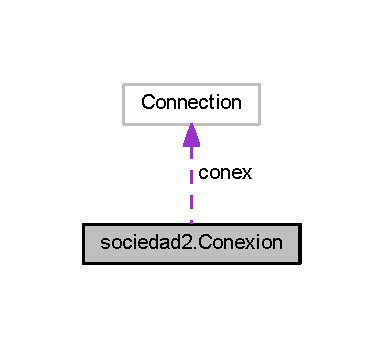
\includegraphics[width=184pt]{classsociedad2_1_1_conexion__coll__graph}
\end{center}
\end{figure}
\subsection*{Public Member Functions}
\begin{DoxyCompactItemize}
\item 
\mbox{\hyperlink{classsociedad2_1_1_conexion_aae3fae24c8652bee72b7b005756aab29}{Conexion}} ()
\item 
Connection \mbox{\hyperlink{classsociedad2_1_1_conexion_ad17987b39ad24b8954e461a5b4412c7b}{crear\+Conexion}} ()
\end{DoxyCompactItemize}


\subsection{Detailed Description}


Definition at line 16 of file Conexion.\+java.



\subsection{Constructor \& Destructor Documentation}
\mbox{\Hypertarget{classsociedad2_1_1_conexion_aae3fae24c8652bee72b7b005756aab29}\label{classsociedad2_1_1_conexion_aae3fae24c8652bee72b7b005756aab29}} 
\index{sociedad2\+::\+Conexion@{sociedad2\+::\+Conexion}!Conexion@{Conexion}}
\index{Conexion@{Conexion}!sociedad2\+::\+Conexion@{sociedad2\+::\+Conexion}}
\subsubsection{\texorpdfstring{Conexion()}{Conexion()}}
{\footnotesize\ttfamily sociedad2.\+Conexion.\+Conexion (\begin{DoxyParamCaption}{ }\end{DoxyParamCaption})}



Definition at line 21 of file Conexion.\+java.



\subsection{Member Function Documentation}
\mbox{\Hypertarget{classsociedad2_1_1_conexion_ad17987b39ad24b8954e461a5b4412c7b}\label{classsociedad2_1_1_conexion_ad17987b39ad24b8954e461a5b4412c7b}} 
\index{sociedad2\+::\+Conexion@{sociedad2\+::\+Conexion}!crear\+Conexion@{crear\+Conexion}}
\index{crear\+Conexion@{crear\+Conexion}!sociedad2\+::\+Conexion@{sociedad2\+::\+Conexion}}
\subsubsection{\texorpdfstring{crear\+Conexion()}{crearConexion()}}
{\footnotesize\ttfamily Connection sociedad2.\+Conexion.\+crear\+Conexion (\begin{DoxyParamCaption}{ }\end{DoxyParamCaption})}



Definition at line 27 of file Conexion.\+java.



The documentation for this class was generated from the following file\+:\begin{DoxyCompactItemize}
\item 
E\+:/eclipse-\/workspace/\+Sociedad/src/sociedad2/\mbox{\hyperlink{_conexion_8java}{Conexion.\+java}}\end{DoxyCompactItemize}

\hypertarget{classsociedad2_1_1_controlador}{}\section{sociedad2.\+Controlador Class Reference}
\label{classsociedad2_1_1_controlador}\index{sociedad2.\+Controlador@{sociedad2.\+Controlador}}


\mbox{\hyperlink{classsociedad2_1_1_controlador}{Controlador}} class.  




Inheritance diagram for sociedad2.\+Controlador\+:\nopagebreak
\begin{figure}[H]
\begin{center}
\leavevmode
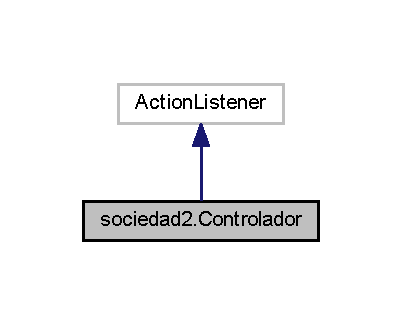
\includegraphics[width=193pt]{classsociedad2_1_1_controlador__inherit__graph}
\end{center}
\end{figure}


Collaboration diagram for sociedad2.\+Controlador\+:
\nopagebreak
\begin{figure}[H]
\begin{center}
\leavevmode
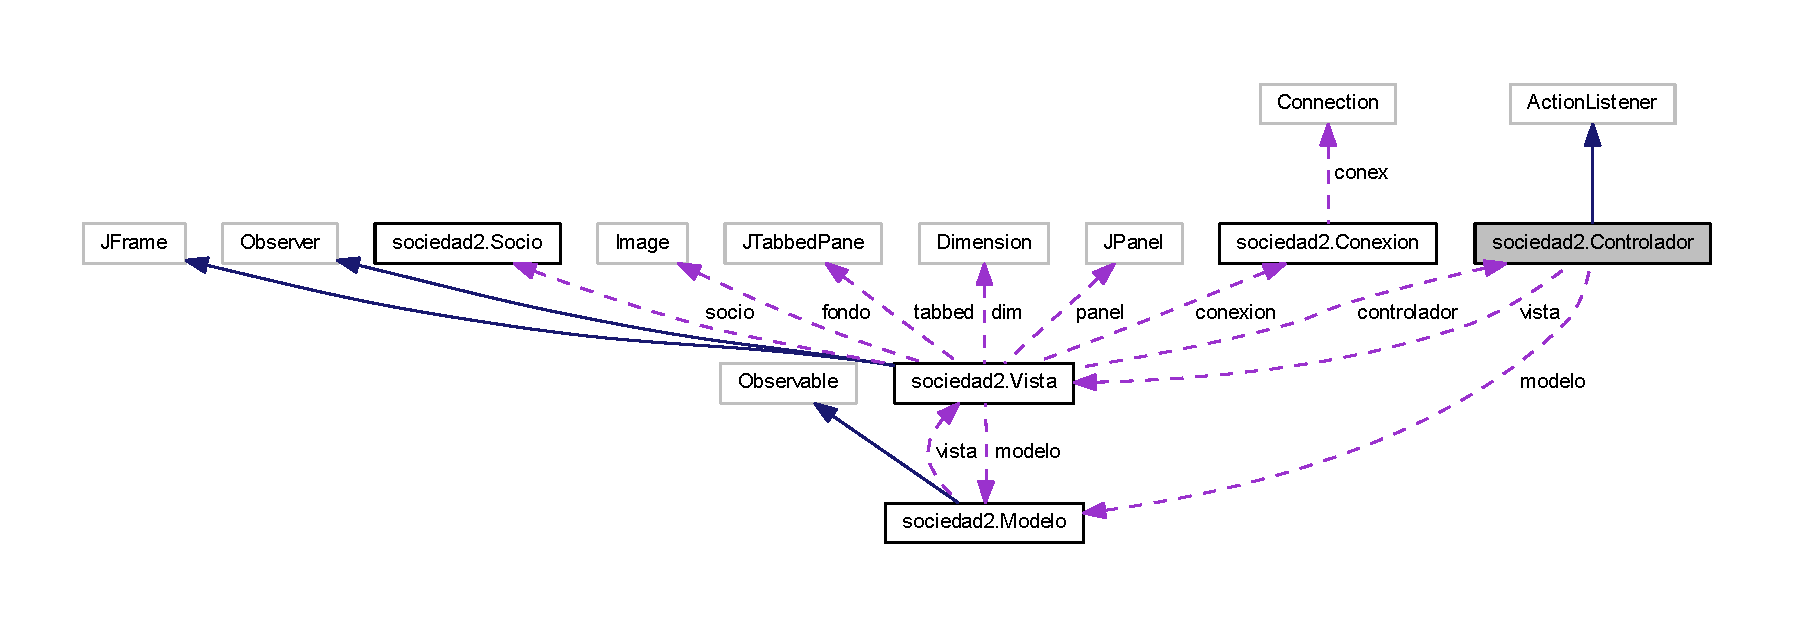
\includegraphics[width=350pt]{classsociedad2_1_1_controlador__coll__graph}
\end{center}
\end{figure}
\subsection*{Public Member Functions}
\begin{DoxyCompactItemize}
\item 
\mbox{\hyperlink{classsociedad2_1_1_controlador_a7601ad3194e4adbe6f760df3ed36c607}{Controlador}} (\mbox{\hyperlink{classsociedad2_1_1_vista}{Vista}} vista, \mbox{\hyperlink{classsociedad2_1_1_modelo}{Modelo}} modelo)
\begin{DoxyCompactList}\small\item\em The constructor of the class \mbox{\hyperlink{classsociedad2_1_1_controlador}{Controlador}}. \end{DoxyCompactList}\item 
void \mbox{\hyperlink{classsociedad2_1_1_controlador_a87860be9c7aff3e6d88d4e88f66e6f51}{action\+Performed}} (Action\+Event e)
\begin{DoxyCompactList}\small\item\em Respond to the actions performed in the interface. \end{DoxyCompactList}\end{DoxyCompactItemize}


\subsection{Detailed Description}
\mbox{\hyperlink{classsociedad2_1_1_controlador}{Controlador}} class. 

Definition at line 27 of file Controlador.\+java.



\subsection{Constructor \& Destructor Documentation}
\mbox{\Hypertarget{classsociedad2_1_1_controlador_a7601ad3194e4adbe6f760df3ed36c607}\label{classsociedad2_1_1_controlador_a7601ad3194e4adbe6f760df3ed36c607}} 
\index{sociedad2\+::\+Controlador@{sociedad2\+::\+Controlador}!Controlador@{Controlador}}
\index{Controlador@{Controlador}!sociedad2\+::\+Controlador@{sociedad2\+::\+Controlador}}
\subsubsection{\texorpdfstring{Controlador()}{Controlador()}}
{\footnotesize\ttfamily sociedad2.\+Controlador.\+Controlador (\begin{DoxyParamCaption}\item[{\mbox{\hyperlink{classsociedad2_1_1_vista}{Vista}}}]{vista,  }\item[{\mbox{\hyperlink{classsociedad2_1_1_modelo}{Modelo}}}]{modelo }\end{DoxyParamCaption})}



The constructor of the class \mbox{\hyperlink{classsociedad2_1_1_controlador}{Controlador}}. 


\begin{DoxyParams}{Parameters}
{\em vista} & Is the \textquotesingle{}main\textquotesingle{} class of the project that represent the interface of the user \\
\hline
{\em modelo} & Handles the data, consulting the database \\
\hline
\end{DoxyParams}


Definition at line 41 of file Controlador.\+java.



\subsection{Member Function Documentation}
\mbox{\Hypertarget{classsociedad2_1_1_controlador_a87860be9c7aff3e6d88d4e88f66e6f51}\label{classsociedad2_1_1_controlador_a87860be9c7aff3e6d88d4e88f66e6f51}} 
\index{sociedad2\+::\+Controlador@{sociedad2\+::\+Controlador}!action\+Performed@{action\+Performed}}
\index{action\+Performed@{action\+Performed}!sociedad2\+::\+Controlador@{sociedad2\+::\+Controlador}}
\subsubsection{\texorpdfstring{action\+Performed()}{actionPerformed()}}
{\footnotesize\ttfamily void sociedad2.\+Controlador.\+action\+Performed (\begin{DoxyParamCaption}\item[{Action\+Event}]{e }\end{DoxyParamCaption})}



Respond to the actions performed in the interface. 


\begin{DoxyParams}{Parameters}
{\em con} & It is the connection between the database and the java program \\
\hline
{\em bai} & It is the id of the registered user \\
\hline
{\em e} & Contains the action that the user want to do \\
\hline
{\em baii} & Contains the id of the last consumption made \\
\hline
{\em i} & Contains the id of the last registered member \\
\hline
{\em a} & Contains the id of the last registered product \\
\hline
{\em dialogo\+Producto} & Opens the interface where we can see the different products of the \textquotesingle{}sociedad\textquotesingle{} \\
\hline
{\em dialogo\+Socio} & Opens the interface where we can see the different members of the \textquotesingle{}sociedad\textquotesingle{} \\
\hline
{\em dialogo\+Ver\+Tu\+Historial} & Opens the interface where we can see the different consumptions made in the \textquotesingle{}sociedad\textquotesingle{} \\
\hline
{\em consumiciones} & Opens the interface where we can register different consumptions that we made in the \textquotesingle{}sociedad\textquotesingle{} \\
\hline
{\em dialogo\+Socio} & Opens the interface where we can register a new member in the \textquotesingle{}sociedad\textquotesingle{} \\
\hline
{\em dialogo\+Producto} & Opens the interface where we can register a new product in the \textquotesingle{}sociedad\textquotesingle{} \\
\hline
{\em dialogo\+Baja} & Opens the interface where we can see the members written off \\
\hline
{\em dialogo\+Prod\+Baja} & Opens the interface where we can see the products written off \\
\hline
\end{DoxyParams}


Definition at line 66 of file Controlador.\+java.



The documentation for this class was generated from the following file\+:\begin{DoxyCompactItemize}
\item 
E\+:/eclipse-\/workspace/\+Sociedad/src/sociedad2/\mbox{\hyperlink{_controlador_8java}{Controlador.\+java}}\end{DoxyCompactItemize}

\hypertarget{classsociedad2_1_1_dialogo_editar_producto}{}\section{sociedad2.\+Dialogo\+Editar\+Producto Class Reference}
\label{classsociedad2_1_1_dialogo_editar_producto}\index{sociedad2.\+Dialogo\+Editar\+Producto@{sociedad2.\+Dialogo\+Editar\+Producto}}


Inheritance diagram for sociedad2.\+Dialogo\+Editar\+Producto\+:
\nopagebreak
\begin{figure}[H]
\begin{center}
\leavevmode
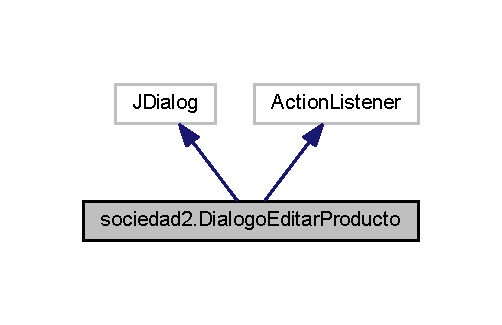
\includegraphics[width=241pt]{classsociedad2_1_1_dialogo_editar_producto__inherit__graph}
\end{center}
\end{figure}


Collaboration diagram for sociedad2.\+Dialogo\+Editar\+Producto\+:
\nopagebreak
\begin{figure}[H]
\begin{center}
\leavevmode
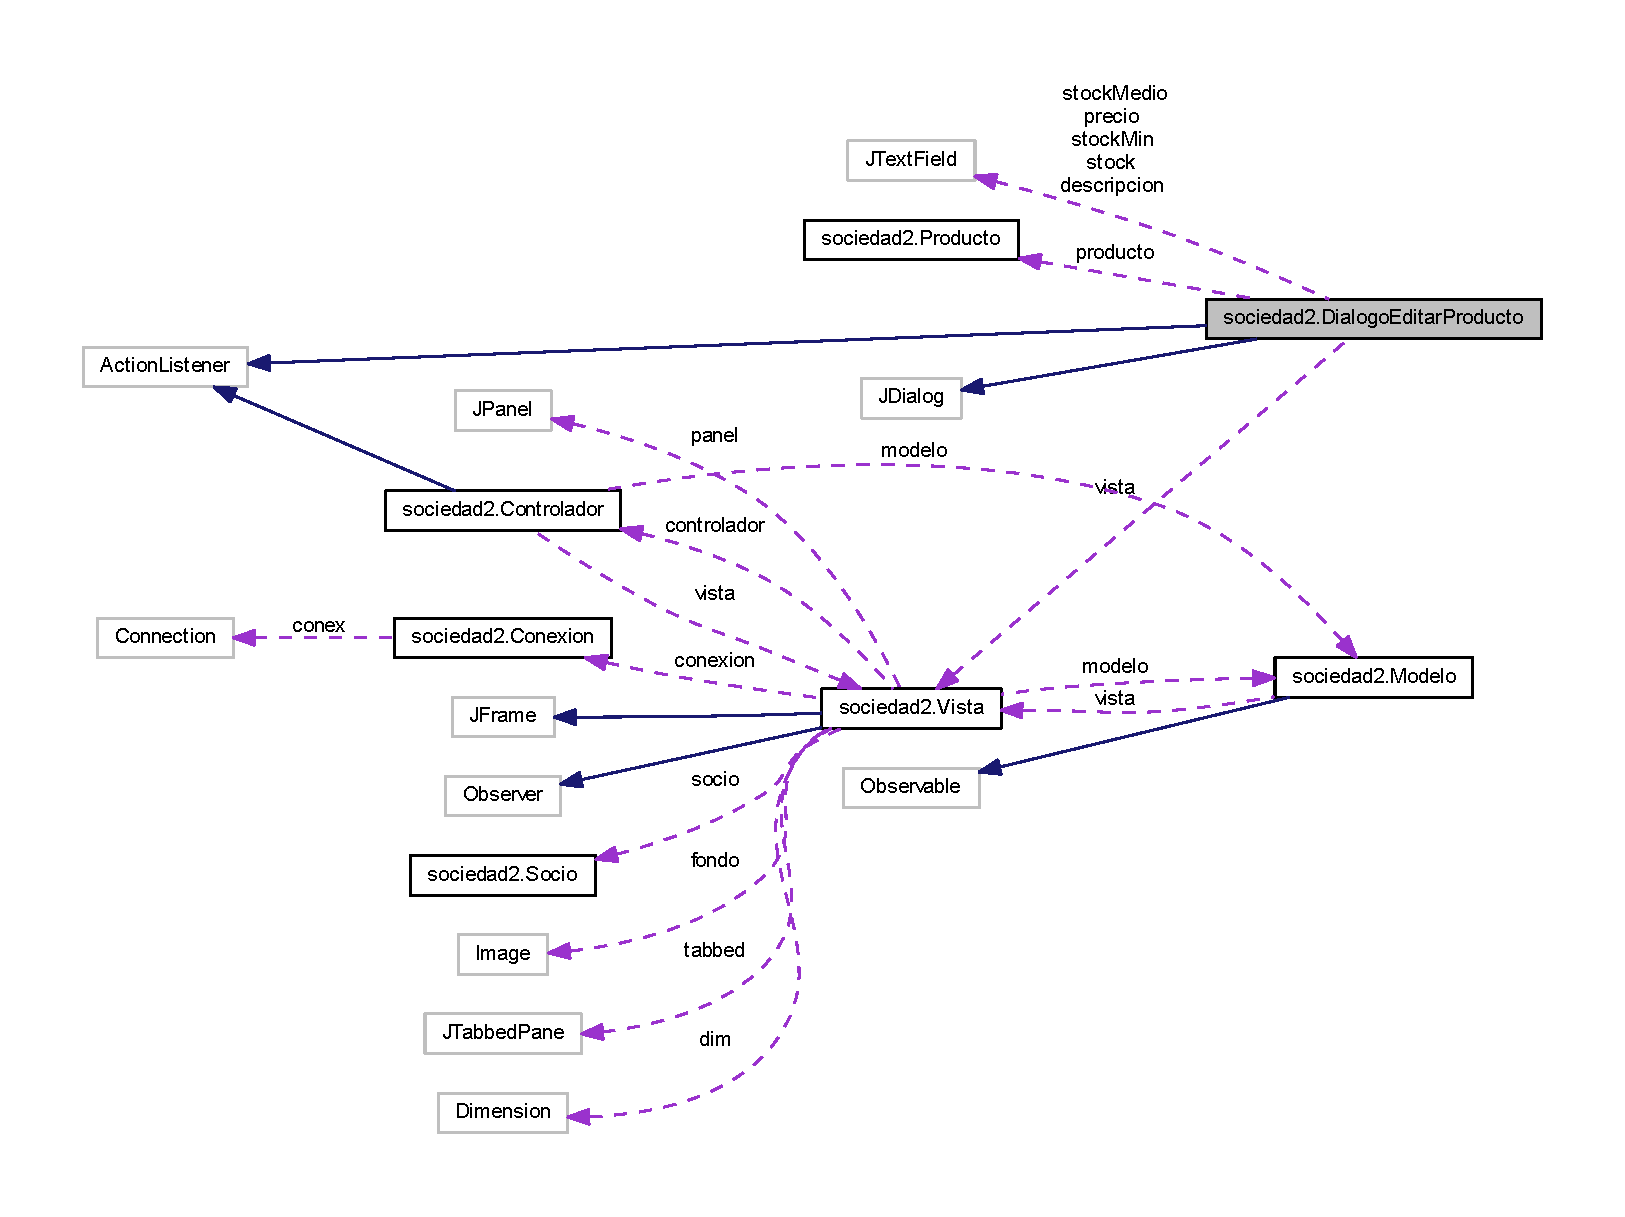
\includegraphics[width=350pt]{classsociedad2_1_1_dialogo_editar_producto__coll__graph}
\end{center}
\end{figure}
\subsection*{Public Member Functions}
\begin{DoxyCompactItemize}
\item 
\mbox{\hyperlink{classsociedad2_1_1_dialogo_editar_producto_affb56a4ab94c03828395eeeb72ec9fda}{Dialogo\+Editar\+Producto}} (\mbox{\hyperlink{classsociedad2_1_1_vista}{Vista}} vista, \mbox{\hyperlink{classsociedad2_1_1_producto}{Producto}} producto)
\item 
void \mbox{\hyperlink{classsociedad2_1_1_dialogo_editar_producto_a98ba8d54ae5c25b8ef24e3f5acd41f27}{action\+Performed}} (Action\+Event e)
\end{DoxyCompactItemize}


\subsection{Detailed Description}


Definition at line 18 of file Dialogo\+Editar\+Producto.\+java.



\subsection{Constructor \& Destructor Documentation}
\mbox{\Hypertarget{classsociedad2_1_1_dialogo_editar_producto_affb56a4ab94c03828395eeeb72ec9fda}\label{classsociedad2_1_1_dialogo_editar_producto_affb56a4ab94c03828395eeeb72ec9fda}} 
\index{sociedad2\+::\+Dialogo\+Editar\+Producto@{sociedad2\+::\+Dialogo\+Editar\+Producto}!Dialogo\+Editar\+Producto@{Dialogo\+Editar\+Producto}}
\index{Dialogo\+Editar\+Producto@{Dialogo\+Editar\+Producto}!sociedad2\+::\+Dialogo\+Editar\+Producto@{sociedad2\+::\+Dialogo\+Editar\+Producto}}
\subsubsection{\texorpdfstring{Dialogo\+Editar\+Producto()}{DialogoEditarProducto()}}
{\footnotesize\ttfamily sociedad2.\+Dialogo\+Editar\+Producto.\+Dialogo\+Editar\+Producto (\begin{DoxyParamCaption}\item[{\mbox{\hyperlink{classsociedad2_1_1_vista}{Vista}}}]{vista,  }\item[{\mbox{\hyperlink{classsociedad2_1_1_producto}{Producto}}}]{producto }\end{DoxyParamCaption})}



Definition at line 25 of file Dialogo\+Editar\+Producto.\+java.



\subsection{Member Function Documentation}
\mbox{\Hypertarget{classsociedad2_1_1_dialogo_editar_producto_a98ba8d54ae5c25b8ef24e3f5acd41f27}\label{classsociedad2_1_1_dialogo_editar_producto_a98ba8d54ae5c25b8ef24e3f5acd41f27}} 
\index{sociedad2\+::\+Dialogo\+Editar\+Producto@{sociedad2\+::\+Dialogo\+Editar\+Producto}!action\+Performed@{action\+Performed}}
\index{action\+Performed@{action\+Performed}!sociedad2\+::\+Dialogo\+Editar\+Producto@{sociedad2\+::\+Dialogo\+Editar\+Producto}}
\subsubsection{\texorpdfstring{action\+Performed()}{actionPerformed()}}
{\footnotesize\ttfamily void sociedad2.\+Dialogo\+Editar\+Producto.\+action\+Performed (\begin{DoxyParamCaption}\item[{Action\+Event}]{e }\end{DoxyParamCaption})}



Definition at line 91 of file Dialogo\+Editar\+Producto.\+java.



The documentation for this class was generated from the following file\+:\begin{DoxyCompactItemize}
\item 
E\+:/eclipse-\/workspace/\+Sociedad/src/sociedad2/\mbox{\hyperlink{_dialogo_editar_producto_8java}{Dialogo\+Editar\+Producto.\+java}}\end{DoxyCompactItemize}

\hypertarget{classsociedad2_1_1_dialogo_editar_socio}{}\section{sociedad2.\+Dialogo\+Editar\+Socio Class Reference}
\label{classsociedad2_1_1_dialogo_editar_socio}\index{sociedad2.\+Dialogo\+Editar\+Socio@{sociedad2.\+Dialogo\+Editar\+Socio}}


Inheritance diagram for sociedad2.\+Dialogo\+Editar\+Socio\+:
\nopagebreak
\begin{figure}[H]
\begin{center}
\leavevmode
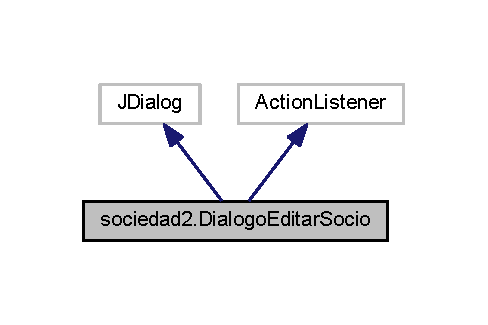
\includegraphics[width=234pt]{classsociedad2_1_1_dialogo_editar_socio__inherit__graph}
\end{center}
\end{figure}


Collaboration diagram for sociedad2.\+Dialogo\+Editar\+Socio\+:
\nopagebreak
\begin{figure}[H]
\begin{center}
\leavevmode
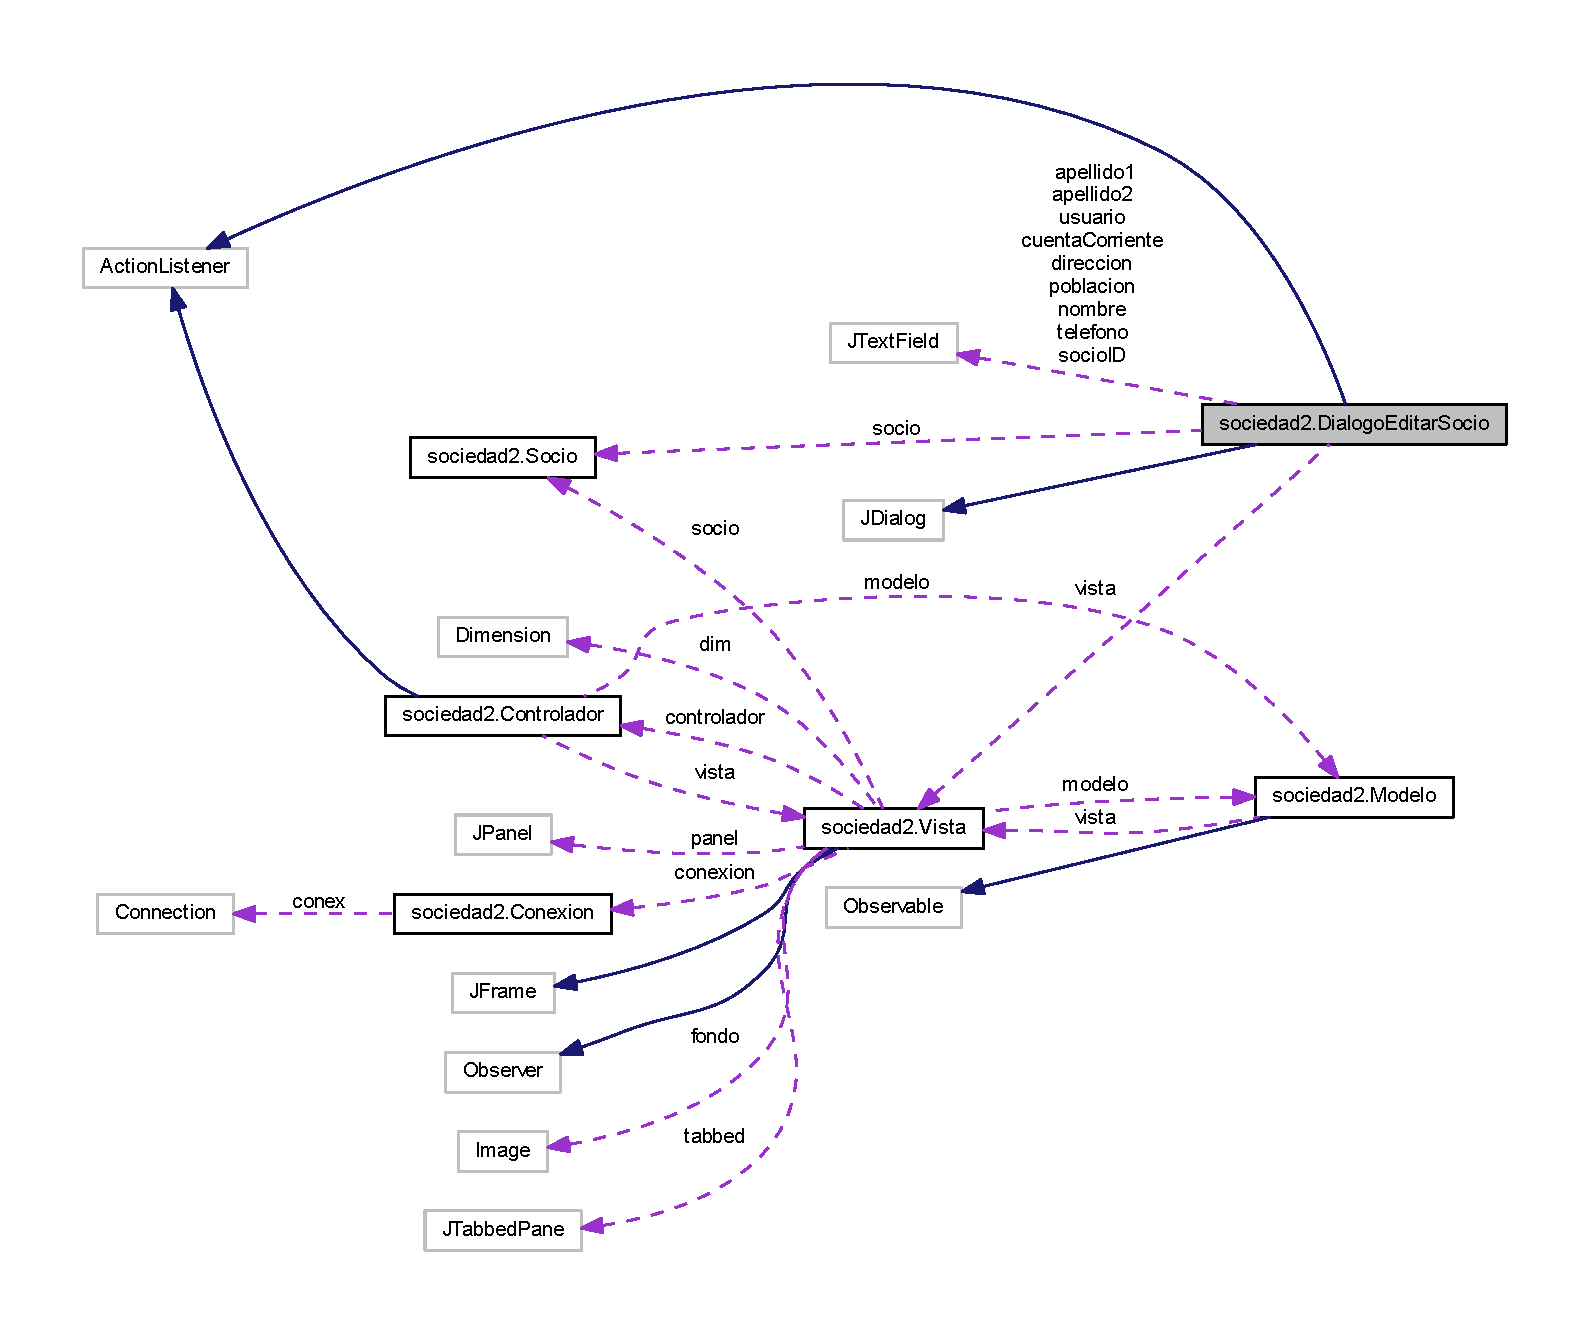
\includegraphics[width=350pt]{classsociedad2_1_1_dialogo_editar_socio__coll__graph}
\end{center}
\end{figure}
\subsection*{Public Member Functions}
\begin{DoxyCompactItemize}
\item 
\mbox{\hyperlink{classsociedad2_1_1_dialogo_editar_socio_aa681ec0932e20367719fe2e7773e81fc}{Dialogo\+Editar\+Socio}} (\mbox{\hyperlink{classsociedad2_1_1_vista}{Vista}} vista, \mbox{\hyperlink{classsociedad2_1_1_socio}{Socio}} socio)
\item 
void \mbox{\hyperlink{classsociedad2_1_1_dialogo_editar_socio_ae3b83db83b25b948c323f63d0efe949d}{action\+Performed}} (Action\+Event e)
\end{DoxyCompactItemize}


\subsection{Detailed Description}


Definition at line 18 of file Dialogo\+Editar\+Socio.\+java.



\subsection{Constructor \& Destructor Documentation}
\mbox{\Hypertarget{classsociedad2_1_1_dialogo_editar_socio_aa681ec0932e20367719fe2e7773e81fc}\label{classsociedad2_1_1_dialogo_editar_socio_aa681ec0932e20367719fe2e7773e81fc}} 
\index{sociedad2\+::\+Dialogo\+Editar\+Socio@{sociedad2\+::\+Dialogo\+Editar\+Socio}!Dialogo\+Editar\+Socio@{Dialogo\+Editar\+Socio}}
\index{Dialogo\+Editar\+Socio@{Dialogo\+Editar\+Socio}!sociedad2\+::\+Dialogo\+Editar\+Socio@{sociedad2\+::\+Dialogo\+Editar\+Socio}}
\subsubsection{\texorpdfstring{Dialogo\+Editar\+Socio()}{DialogoEditarSocio()}}
{\footnotesize\ttfamily sociedad2.\+Dialogo\+Editar\+Socio.\+Dialogo\+Editar\+Socio (\begin{DoxyParamCaption}\item[{\mbox{\hyperlink{classsociedad2_1_1_vista}{Vista}}}]{vista,  }\item[{\mbox{\hyperlink{classsociedad2_1_1_socio}{Socio}}}]{socio }\end{DoxyParamCaption})}



Definition at line 25 of file Dialogo\+Editar\+Socio.\+java.



\subsection{Member Function Documentation}
\mbox{\Hypertarget{classsociedad2_1_1_dialogo_editar_socio_ae3b83db83b25b948c323f63d0efe949d}\label{classsociedad2_1_1_dialogo_editar_socio_ae3b83db83b25b948c323f63d0efe949d}} 
\index{sociedad2\+::\+Dialogo\+Editar\+Socio@{sociedad2\+::\+Dialogo\+Editar\+Socio}!action\+Performed@{action\+Performed}}
\index{action\+Performed@{action\+Performed}!sociedad2\+::\+Dialogo\+Editar\+Socio@{sociedad2\+::\+Dialogo\+Editar\+Socio}}
\subsubsection{\texorpdfstring{action\+Performed()}{actionPerformed()}}
{\footnotesize\ttfamily void sociedad2.\+Dialogo\+Editar\+Socio.\+action\+Performed (\begin{DoxyParamCaption}\item[{Action\+Event}]{e }\end{DoxyParamCaption})}



Definition at line 96 of file Dialogo\+Editar\+Socio.\+java.



The documentation for this class was generated from the following file\+:\begin{DoxyCompactItemize}
\item 
E\+:/eclipse-\/workspace/\+Sociedad/src/sociedad2/\mbox{\hyperlink{_dialogo_editar_socio_8java}{Dialogo\+Editar\+Socio.\+java}}\end{DoxyCompactItemize}

\hypertarget{classsociedad2_1_1_dialogo_insertar_producto}{}\section{sociedad2.\+Dialogo\+Insertar\+Producto Class Reference}
\label{classsociedad2_1_1_dialogo_insertar_producto}\index{sociedad2.\+Dialogo\+Insertar\+Producto@{sociedad2.\+Dialogo\+Insertar\+Producto}}


Inheritance diagram for sociedad2.\+Dialogo\+Insertar\+Producto\+:\nopagebreak
\begin{figure}[H]
\begin{center}
\leavevmode
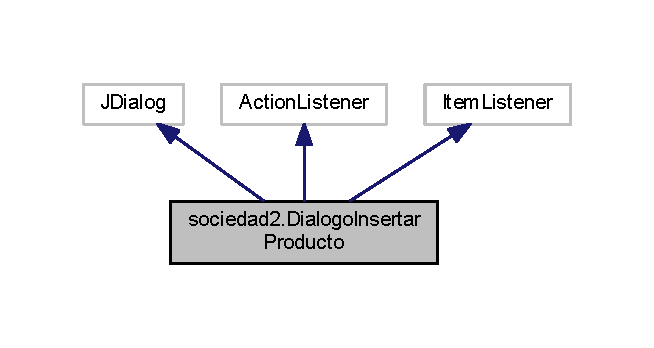
\includegraphics[width=314pt]{classsociedad2_1_1_dialogo_insertar_producto__inherit__graph}
\end{center}
\end{figure}


Collaboration diagram for sociedad2.\+Dialogo\+Insertar\+Producto\+:
\nopagebreak
\begin{figure}[H]
\begin{center}
\leavevmode
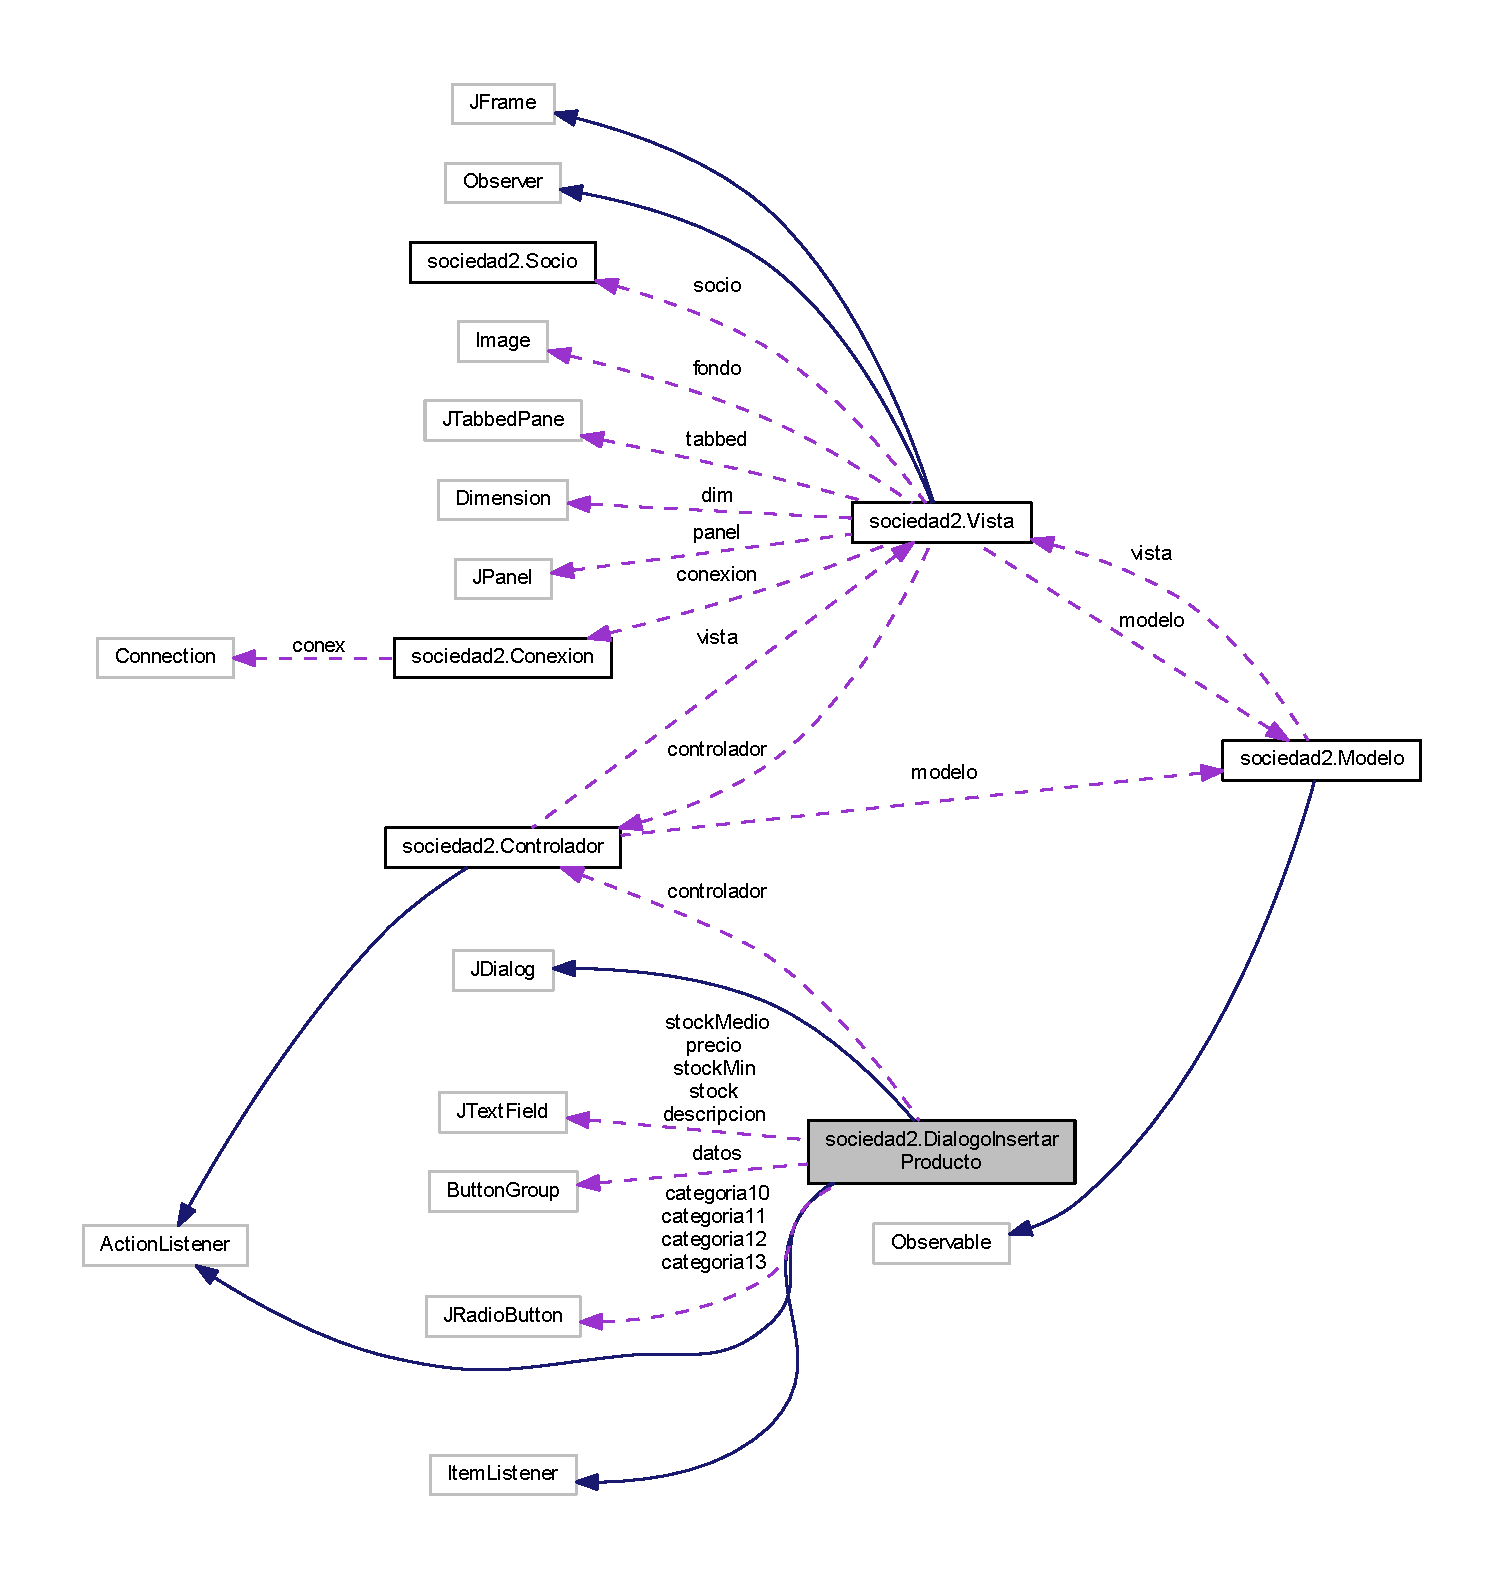
\includegraphics[width=350pt]{classsociedad2_1_1_dialogo_insertar_producto__coll__graph}
\end{center}
\end{figure}
\subsection*{Public Member Functions}
\begin{DoxyCompactItemize}
\item 
\mbox{\hyperlink{classsociedad2_1_1_dialogo_insertar_producto_a515496f2391bbc8216171f48da3a45c6}{Dialogo\+Insertar\+Producto}} (\mbox{\hyperlink{classsociedad2_1_1_controlador}{Controlador}} controlador, int i)
\item 
Container \mbox{\hyperlink{classsociedad2_1_1_dialogo_insertar_producto_aee7461340b7391e53ca39a6d72fb9ded}{crear\+Grupo\+Boton}} (String titulo)
\item 
void \mbox{\hyperlink{classsociedad2_1_1_dialogo_insertar_producto_a96b7d9145151ddc6ce20fe20acaa79e9}{action\+Performed}} (Action\+Event e)
\item 
void \mbox{\hyperlink{classsociedad2_1_1_dialogo_insertar_producto_a961e22b3de549ec4609e9a2c41670b98}{item\+State\+Changed}} (Item\+Event e)
\end{DoxyCompactItemize}


\subsection{Detailed Description}


Definition at line 23 of file Dialogo\+Insertar\+Producto.\+java.



\subsection{Constructor \& Destructor Documentation}
\mbox{\Hypertarget{classsociedad2_1_1_dialogo_insertar_producto_a515496f2391bbc8216171f48da3a45c6}\label{classsociedad2_1_1_dialogo_insertar_producto_a515496f2391bbc8216171f48da3a45c6}} 
\index{sociedad2\+::\+Dialogo\+Insertar\+Producto@{sociedad2\+::\+Dialogo\+Insertar\+Producto}!Dialogo\+Insertar\+Producto@{Dialogo\+Insertar\+Producto}}
\index{Dialogo\+Insertar\+Producto@{Dialogo\+Insertar\+Producto}!sociedad2\+::\+Dialogo\+Insertar\+Producto@{sociedad2\+::\+Dialogo\+Insertar\+Producto}}
\subsubsection{\texorpdfstring{Dialogo\+Insertar\+Producto()}{DialogoInsertarProducto()}}
{\footnotesize\ttfamily sociedad2.\+Dialogo\+Insertar\+Producto.\+Dialogo\+Insertar\+Producto (\begin{DoxyParamCaption}\item[{\mbox{\hyperlink{classsociedad2_1_1_controlador}{Controlador}}}]{controlador,  }\item[{int}]{i }\end{DoxyParamCaption})}



Definition at line 33 of file Dialogo\+Insertar\+Producto.\+java.



\subsection{Member Function Documentation}
\mbox{\Hypertarget{classsociedad2_1_1_dialogo_insertar_producto_a96b7d9145151ddc6ce20fe20acaa79e9}\label{classsociedad2_1_1_dialogo_insertar_producto_a96b7d9145151ddc6ce20fe20acaa79e9}} 
\index{sociedad2\+::\+Dialogo\+Insertar\+Producto@{sociedad2\+::\+Dialogo\+Insertar\+Producto}!action\+Performed@{action\+Performed}}
\index{action\+Performed@{action\+Performed}!sociedad2\+::\+Dialogo\+Insertar\+Producto@{sociedad2\+::\+Dialogo\+Insertar\+Producto}}
\subsubsection{\texorpdfstring{action\+Performed()}{actionPerformed()}}
{\footnotesize\ttfamily void sociedad2.\+Dialogo\+Insertar\+Producto.\+action\+Performed (\begin{DoxyParamCaption}\item[{Action\+Event}]{e }\end{DoxyParamCaption})}



Definition at line 146 of file Dialogo\+Insertar\+Producto.\+java.

\mbox{\Hypertarget{classsociedad2_1_1_dialogo_insertar_producto_aee7461340b7391e53ca39a6d72fb9ded}\label{classsociedad2_1_1_dialogo_insertar_producto_aee7461340b7391e53ca39a6d72fb9ded}} 
\index{sociedad2\+::\+Dialogo\+Insertar\+Producto@{sociedad2\+::\+Dialogo\+Insertar\+Producto}!crear\+Grupo\+Boton@{crear\+Grupo\+Boton}}
\index{crear\+Grupo\+Boton@{crear\+Grupo\+Boton}!sociedad2\+::\+Dialogo\+Insertar\+Producto@{sociedad2\+::\+Dialogo\+Insertar\+Producto}}
\subsubsection{\texorpdfstring{crear\+Grupo\+Boton()}{crearGrupoBoton()}}
{\footnotesize\ttfamily Container sociedad2.\+Dialogo\+Insertar\+Producto.\+crear\+Grupo\+Boton (\begin{DoxyParamCaption}\item[{String}]{titulo }\end{DoxyParamCaption})}



Definition at line 54 of file Dialogo\+Insertar\+Producto.\+java.

\mbox{\Hypertarget{classsociedad2_1_1_dialogo_insertar_producto_a961e22b3de549ec4609e9a2c41670b98}\label{classsociedad2_1_1_dialogo_insertar_producto_a961e22b3de549ec4609e9a2c41670b98}} 
\index{sociedad2\+::\+Dialogo\+Insertar\+Producto@{sociedad2\+::\+Dialogo\+Insertar\+Producto}!item\+State\+Changed@{item\+State\+Changed}}
\index{item\+State\+Changed@{item\+State\+Changed}!sociedad2\+::\+Dialogo\+Insertar\+Producto@{sociedad2\+::\+Dialogo\+Insertar\+Producto}}
\subsubsection{\texorpdfstring{item\+State\+Changed()}{itemStateChanged()}}
{\footnotesize\ttfamily void sociedad2.\+Dialogo\+Insertar\+Producto.\+item\+State\+Changed (\begin{DoxyParamCaption}\item[{Item\+Event}]{e }\end{DoxyParamCaption})}



Definition at line 192 of file Dialogo\+Insertar\+Producto.\+java.



The documentation for this class was generated from the following file\+:\begin{DoxyCompactItemize}
\item 
E\+:/eclipse-\/workspace/\+Sociedad/src/sociedad2/\mbox{\hyperlink{_dialogo_insertar_producto_8java}{Dialogo\+Insertar\+Producto.\+java}}\end{DoxyCompactItemize}

\hypertarget{classsociedad2_1_1_dialogo_insertar_socio}{}\section{sociedad2.\+Dialogo\+Insertar\+Socio Class Reference}
\label{classsociedad2_1_1_dialogo_insertar_socio}\index{sociedad2.\+Dialogo\+Insertar\+Socio@{sociedad2.\+Dialogo\+Insertar\+Socio}}


Inheritance diagram for sociedad2.\+Dialogo\+Insertar\+Socio\+:
\nopagebreak
\begin{figure}[H]
\begin{center}
\leavevmode
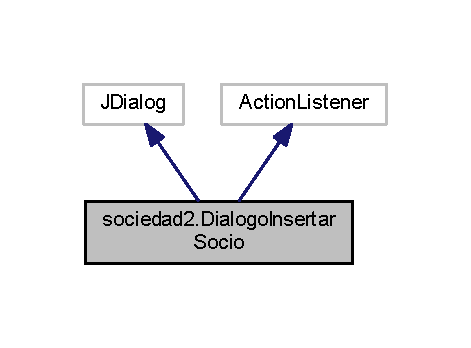
\includegraphics[width=226pt]{classsociedad2_1_1_dialogo_insertar_socio__inherit__graph}
\end{center}
\end{figure}


Collaboration diagram for sociedad2.\+Dialogo\+Insertar\+Socio\+:
\nopagebreak
\begin{figure}[H]
\begin{center}
\leavevmode
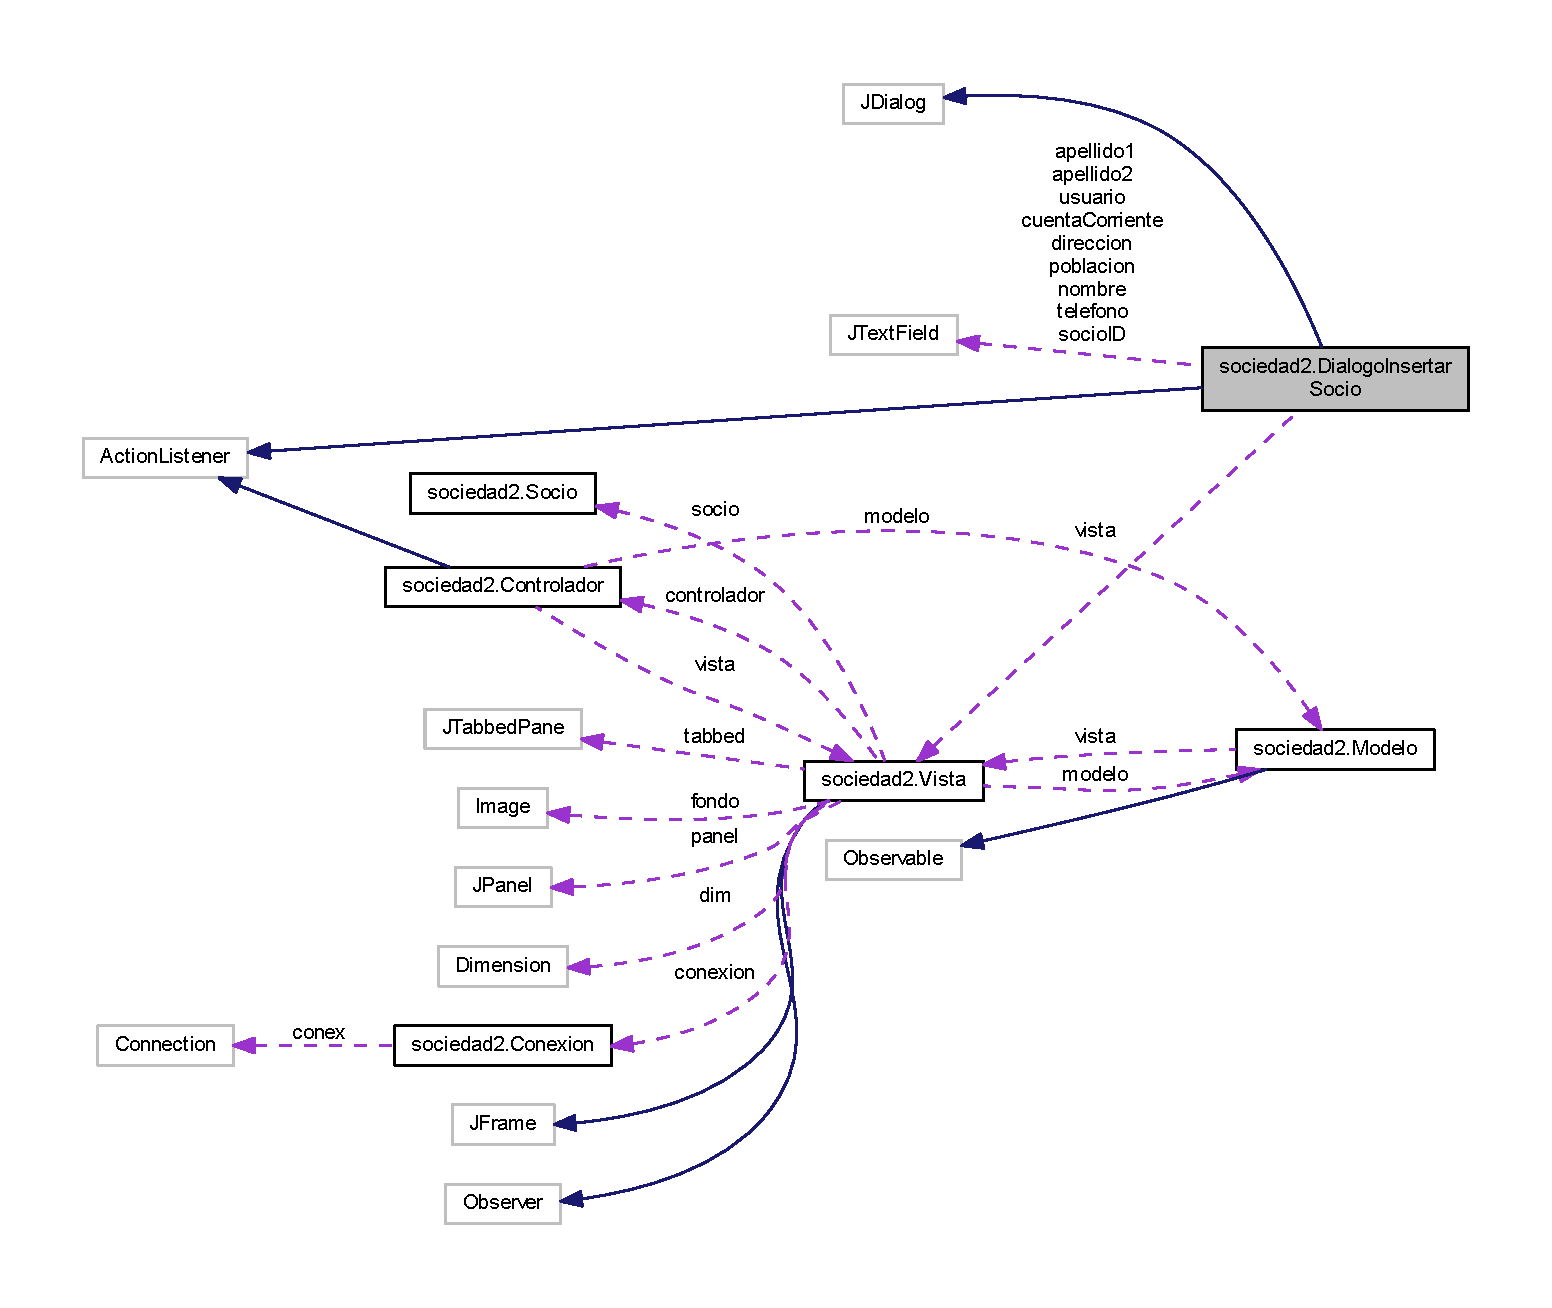
\includegraphics[width=350pt]{classsociedad2_1_1_dialogo_insertar_socio__coll__graph}
\end{center}
\end{figure}
\subsection*{Public Member Functions}
\begin{DoxyCompactItemize}
\item 
\mbox{\hyperlink{classsociedad2_1_1_dialogo_insertar_socio_a1467bf782876cdc9424744d6eafaad4e}{Dialogo\+Insertar\+Socio}} (\mbox{\hyperlink{classsociedad2_1_1_vista}{Vista}} vista, int id)
\item 
void \mbox{\hyperlink{classsociedad2_1_1_dialogo_insertar_socio_a8cff370d2d035c22b84b0257391ff93f}{action\+Performed}} (Action\+Event e)
\end{DoxyCompactItemize}


\subsection{Detailed Description}


Definition at line 20 of file Dialogo\+Insertar\+Socio.\+java.



\subsection{Constructor \& Destructor Documentation}
\mbox{\Hypertarget{classsociedad2_1_1_dialogo_insertar_socio_a1467bf782876cdc9424744d6eafaad4e}\label{classsociedad2_1_1_dialogo_insertar_socio_a1467bf782876cdc9424744d6eafaad4e}} 
\index{sociedad2\+::\+Dialogo\+Insertar\+Socio@{sociedad2\+::\+Dialogo\+Insertar\+Socio}!Dialogo\+Insertar\+Socio@{Dialogo\+Insertar\+Socio}}
\index{Dialogo\+Insertar\+Socio@{Dialogo\+Insertar\+Socio}!sociedad2\+::\+Dialogo\+Insertar\+Socio@{sociedad2\+::\+Dialogo\+Insertar\+Socio}}
\subsubsection{\texorpdfstring{Dialogo\+Insertar\+Socio()}{DialogoInsertarSocio()}}
{\footnotesize\ttfamily sociedad2.\+Dialogo\+Insertar\+Socio.\+Dialogo\+Insertar\+Socio (\begin{DoxyParamCaption}\item[{\mbox{\hyperlink{classsociedad2_1_1_vista}{Vista}}}]{vista,  }\item[{int}]{id }\end{DoxyParamCaption})}



Definition at line 27 of file Dialogo\+Insertar\+Socio.\+java.



\subsection{Member Function Documentation}
\mbox{\Hypertarget{classsociedad2_1_1_dialogo_insertar_socio_a8cff370d2d035c22b84b0257391ff93f}\label{classsociedad2_1_1_dialogo_insertar_socio_a8cff370d2d035c22b84b0257391ff93f}} 
\index{sociedad2\+::\+Dialogo\+Insertar\+Socio@{sociedad2\+::\+Dialogo\+Insertar\+Socio}!action\+Performed@{action\+Performed}}
\index{action\+Performed@{action\+Performed}!sociedad2\+::\+Dialogo\+Insertar\+Socio@{sociedad2\+::\+Dialogo\+Insertar\+Socio}}
\subsubsection{\texorpdfstring{action\+Performed()}{actionPerformed()}}
{\footnotesize\ttfamily void sociedad2.\+Dialogo\+Insertar\+Socio.\+action\+Performed (\begin{DoxyParamCaption}\item[{Action\+Event}]{e }\end{DoxyParamCaption})}



Definition at line 97 of file Dialogo\+Insertar\+Socio.\+java.



The documentation for this class was generated from the following file\+:\begin{DoxyCompactItemize}
\item 
E\+:/eclipse-\/workspace/\+Sociedad/src/sociedad2/\mbox{\hyperlink{_dialogo_insertar_socio_8java}{Dialogo\+Insertar\+Socio.\+java}}\end{DoxyCompactItemize}

\hypertarget{classsociedad2_1_1_dialogo_registrar_consumicion}{}\section{sociedad2.\+Dialogo\+Registrar\+Consumicion Class Reference}
\label{classsociedad2_1_1_dialogo_registrar_consumicion}\index{sociedad2.\+Dialogo\+Registrar\+Consumicion@{sociedad2.\+Dialogo\+Registrar\+Consumicion}}


Inheritance diagram for sociedad2.\+Dialogo\+Registrar\+Consumicion\+:
\nopagebreak
\begin{figure}[H]
\begin{center}
\leavevmode
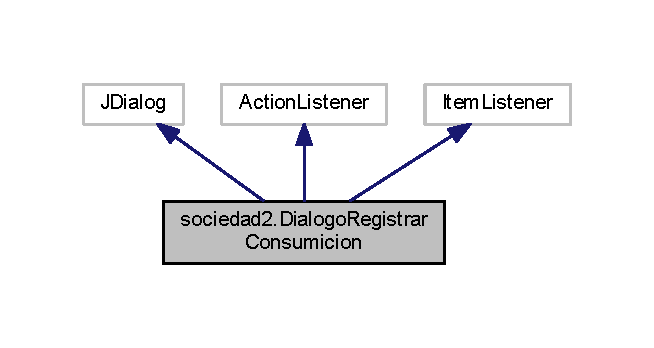
\includegraphics[width=314pt]{classsociedad2_1_1_dialogo_registrar_consumicion__inherit__graph}
\end{center}
\end{figure}


Collaboration diagram for sociedad2.\+Dialogo\+Registrar\+Consumicion\+:
\nopagebreak
\begin{figure}[H]
\begin{center}
\leavevmode
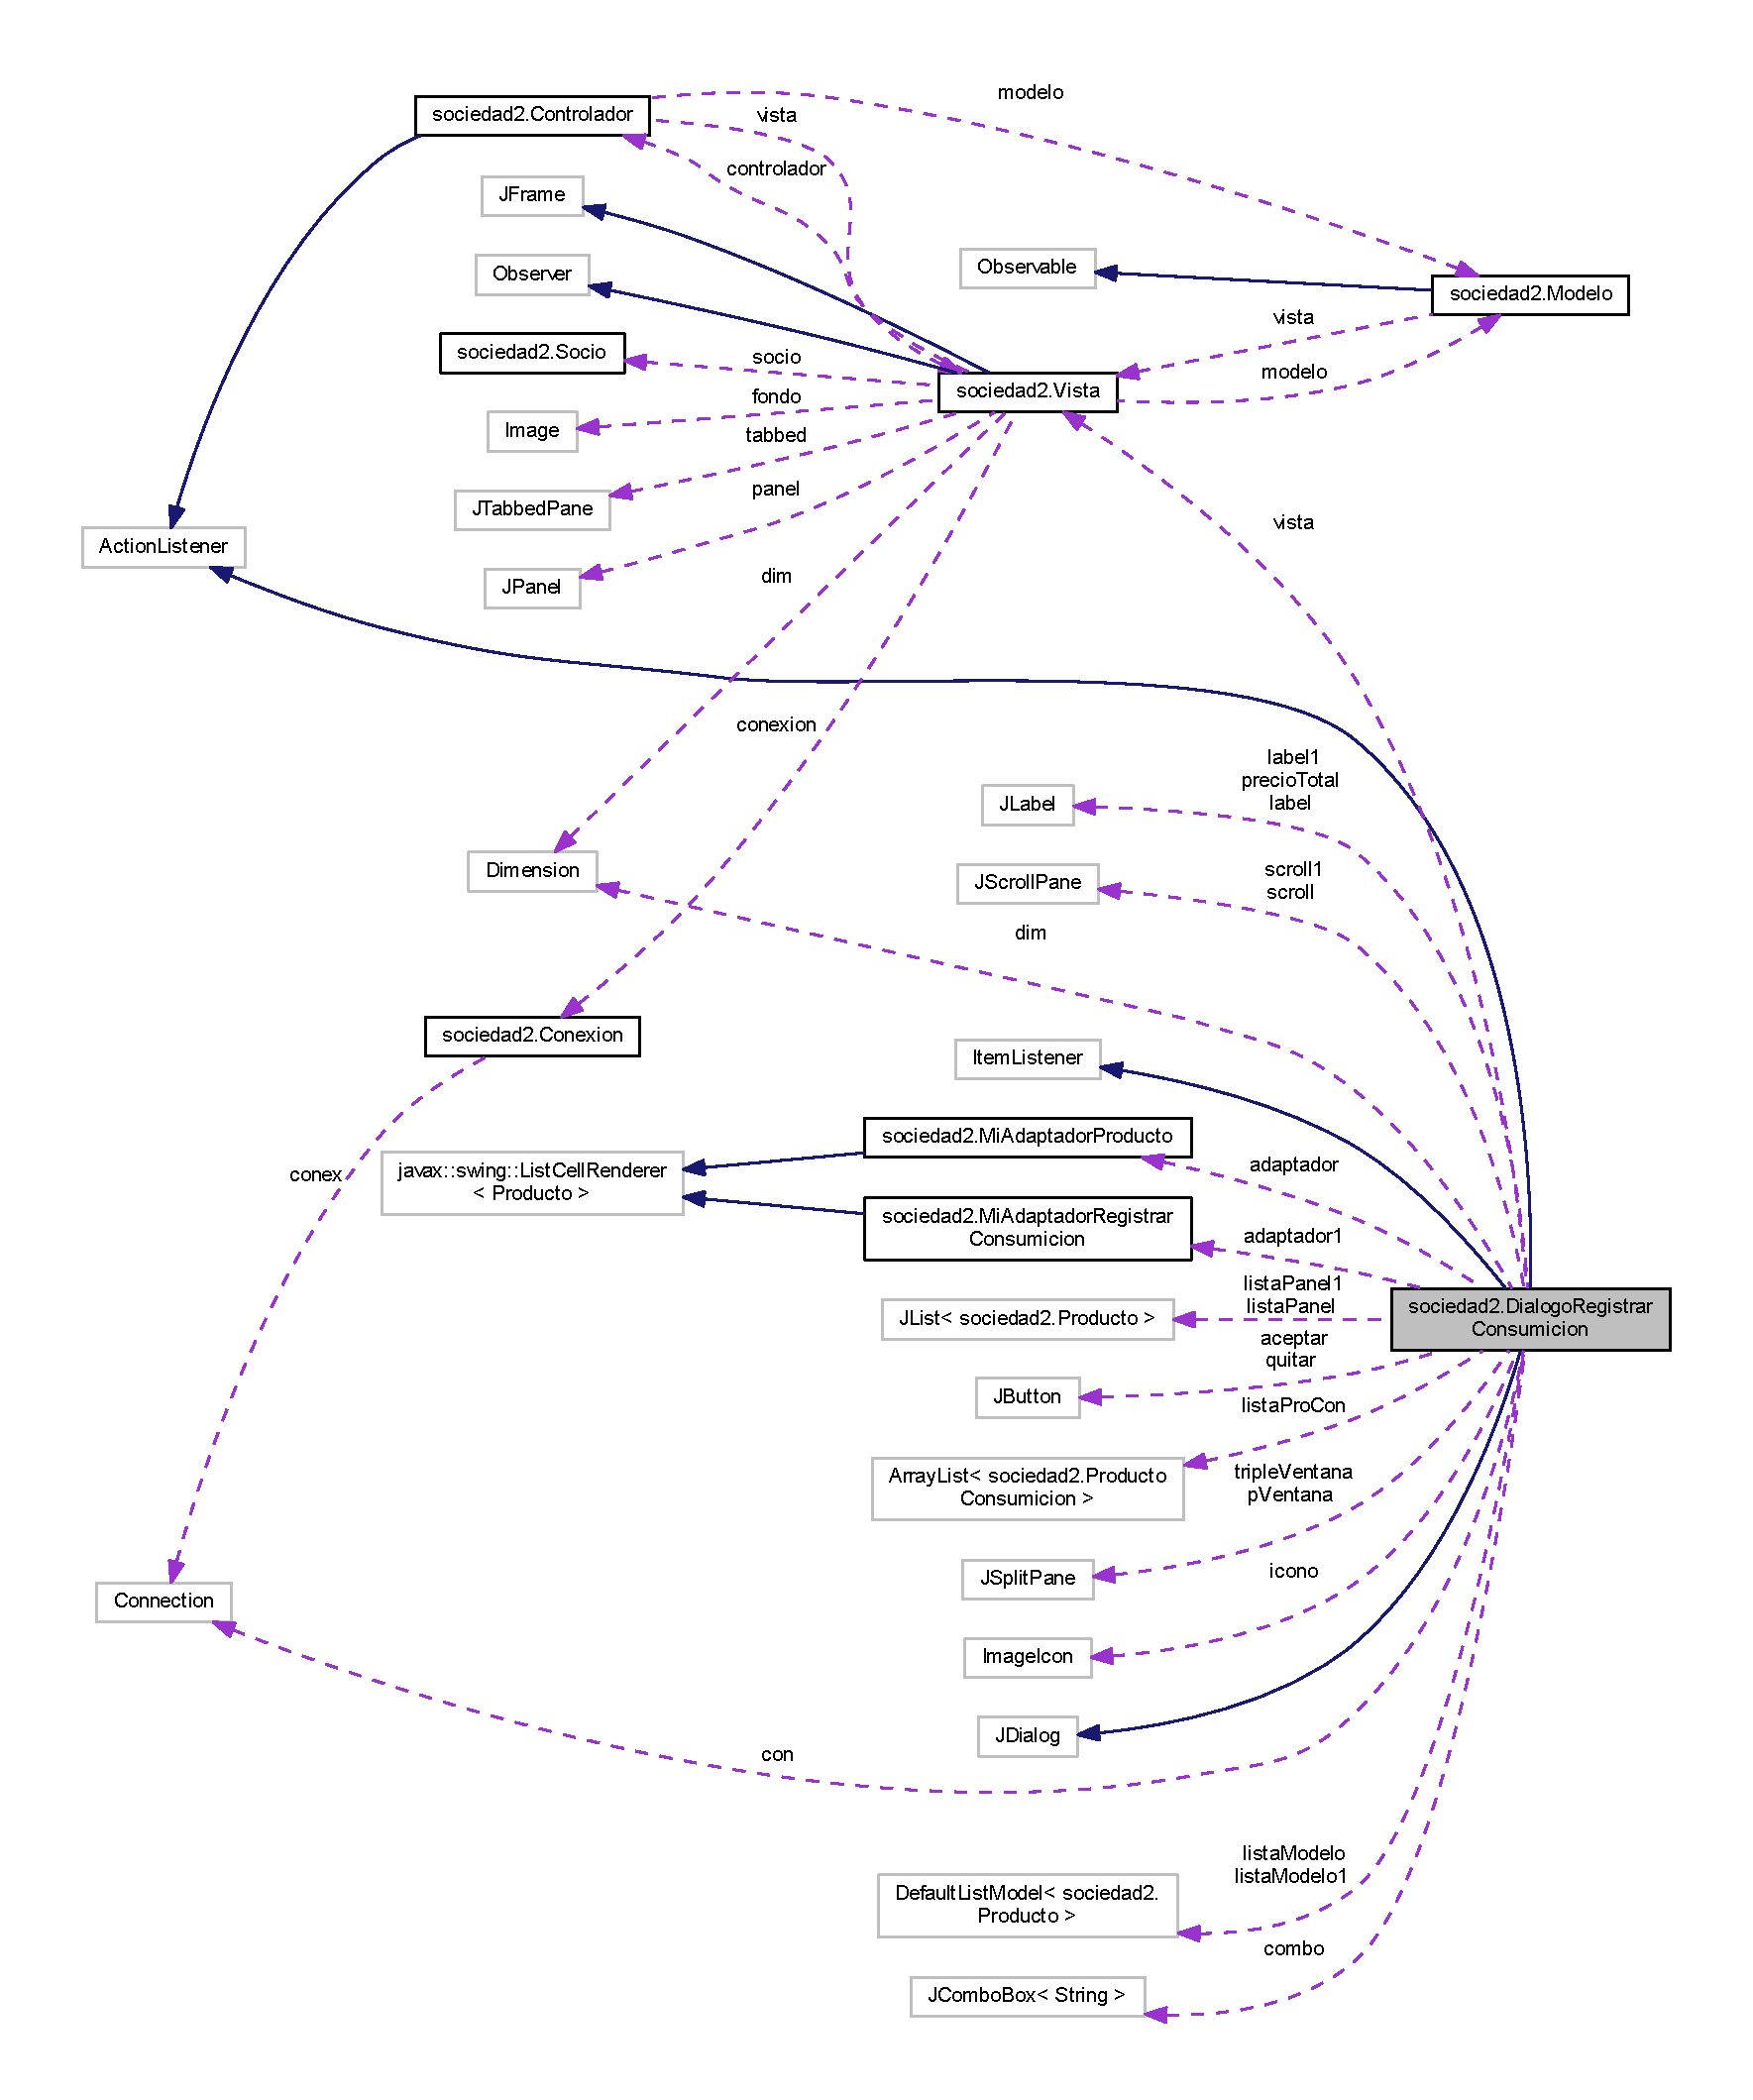
\includegraphics[width=350pt]{classsociedad2_1_1_dialogo_registrar_consumicion__coll__graph}
\end{center}
\end{figure}
\subsection*{Public Member Functions}
\begin{DoxyCompactItemize}
\item 
\mbox{\hyperlink{classsociedad2_1_1_dialogo_registrar_consumicion_a259e56e9b3494e7d1fc134370ec362dd}{Dialogo\+Registrar\+Consumicion}} (\mbox{\hyperlink{classsociedad2_1_1_vista}{Vista}} vista, String comando, String info, Connection con)  throws S\+Q\+L\+Exception 
\item 
Component \mbox{\hyperlink{classsociedad2_1_1_dialogo_registrar_consumicion_a03abf39f1f7ad719daf309e2507e8fe2}{crear\+Panel\+Scroll}} ()  throws S\+Q\+L\+Exception 
\item 
Container \mbox{\hyperlink{classsociedad2_1_1_dialogo_registrar_consumicion_a5b6ab708bcc0b27ef9a3ffcb557e4356}{crear\+Botones}} (String titulo)
\item 
Container \mbox{\hyperlink{classsociedad2_1_1_dialogo_registrar_consumicion_a5597a3fa2f6b7e7a6b6c1c4893b2875a}{crear\+Panel\+Botones}} ()
\item 
Container \mbox{\hyperlink{classsociedad2_1_1_dialogo_registrar_consumicion_a13951c3941ceda5aca796fea7d93d6d4}{crear\+Panel\+Contador}} ()
\item 
\mbox{\hyperlink{classsociedad2_1_1_producto}{Producto}} \mbox{\hyperlink{classsociedad2_1_1_dialogo_registrar_consumicion_a59a8cdd15d8fe30b30d0f11df3b68b8d}{resert\+Stock}} (\mbox{\hyperlink{classsociedad2_1_1_producto}{Producto}} producto)
\item 
void \mbox{\hyperlink{classsociedad2_1_1_dialogo_registrar_consumicion_a0910cb6ece7188ee98dc8c972f0c453a}{action\+Performed}} (Action\+Event e)
\item 
void \mbox{\hyperlink{classsociedad2_1_1_dialogo_registrar_consumicion_a136409604ab04264d7a00dd5bf4752af}{item\+State\+Changed}} (Item\+Event e)
\end{DoxyCompactItemize}


\subsection{Detailed Description}


Definition at line 31 of file Dialogo\+Registrar\+Consumicion.\+java.



\subsection{Constructor \& Destructor Documentation}
\mbox{\Hypertarget{classsociedad2_1_1_dialogo_registrar_consumicion_a259e56e9b3494e7d1fc134370ec362dd}\label{classsociedad2_1_1_dialogo_registrar_consumicion_a259e56e9b3494e7d1fc134370ec362dd}} 
\index{sociedad2\+::\+Dialogo\+Registrar\+Consumicion@{sociedad2\+::\+Dialogo\+Registrar\+Consumicion}!Dialogo\+Registrar\+Consumicion@{Dialogo\+Registrar\+Consumicion}}
\index{Dialogo\+Registrar\+Consumicion@{Dialogo\+Registrar\+Consumicion}!sociedad2\+::\+Dialogo\+Registrar\+Consumicion@{sociedad2\+::\+Dialogo\+Registrar\+Consumicion}}
\subsubsection{\texorpdfstring{Dialogo\+Registrar\+Consumicion()}{DialogoRegistrarConsumicion()}}
{\footnotesize\ttfamily sociedad2.\+Dialogo\+Registrar\+Consumicion.\+Dialogo\+Registrar\+Consumicion (\begin{DoxyParamCaption}\item[{\mbox{\hyperlink{classsociedad2_1_1_vista}{Vista}}}]{vista,  }\item[{String}]{comando,  }\item[{String}]{info,  }\item[{Connection}]{con }\end{DoxyParamCaption}) throws S\+Q\+L\+Exception}



Definition at line 57 of file Dialogo\+Registrar\+Consumicion.\+java.



\subsection{Member Function Documentation}
\mbox{\Hypertarget{classsociedad2_1_1_dialogo_registrar_consumicion_a0910cb6ece7188ee98dc8c972f0c453a}\label{classsociedad2_1_1_dialogo_registrar_consumicion_a0910cb6ece7188ee98dc8c972f0c453a}} 
\index{sociedad2\+::\+Dialogo\+Registrar\+Consumicion@{sociedad2\+::\+Dialogo\+Registrar\+Consumicion}!action\+Performed@{action\+Performed}}
\index{action\+Performed@{action\+Performed}!sociedad2\+::\+Dialogo\+Registrar\+Consumicion@{sociedad2\+::\+Dialogo\+Registrar\+Consumicion}}
\subsubsection{\texorpdfstring{action\+Performed()}{actionPerformed()}}
{\footnotesize\ttfamily void sociedad2.\+Dialogo\+Registrar\+Consumicion.\+action\+Performed (\begin{DoxyParamCaption}\item[{Action\+Event}]{e }\end{DoxyParamCaption})}



Definition at line 278 of file Dialogo\+Registrar\+Consumicion.\+java.

\mbox{\Hypertarget{classsociedad2_1_1_dialogo_registrar_consumicion_a5b6ab708bcc0b27ef9a3ffcb557e4356}\label{classsociedad2_1_1_dialogo_registrar_consumicion_a5b6ab708bcc0b27ef9a3ffcb557e4356}} 
\index{sociedad2\+::\+Dialogo\+Registrar\+Consumicion@{sociedad2\+::\+Dialogo\+Registrar\+Consumicion}!crear\+Botones@{crear\+Botones}}
\index{crear\+Botones@{crear\+Botones}!sociedad2\+::\+Dialogo\+Registrar\+Consumicion@{sociedad2\+::\+Dialogo\+Registrar\+Consumicion}}
\subsubsection{\texorpdfstring{crear\+Botones()}{crearBotones()}}
{\footnotesize\ttfamily Container sociedad2.\+Dialogo\+Registrar\+Consumicion.\+crear\+Botones (\begin{DoxyParamCaption}\item[{String}]{titulo }\end{DoxyParamCaption})}



Definition at line 184 of file Dialogo\+Registrar\+Consumicion.\+java.

\mbox{\Hypertarget{classsociedad2_1_1_dialogo_registrar_consumicion_a5597a3fa2f6b7e7a6b6c1c4893b2875a}\label{classsociedad2_1_1_dialogo_registrar_consumicion_a5597a3fa2f6b7e7a6b6c1c4893b2875a}} 
\index{sociedad2\+::\+Dialogo\+Registrar\+Consumicion@{sociedad2\+::\+Dialogo\+Registrar\+Consumicion}!crear\+Panel\+Botones@{crear\+Panel\+Botones}}
\index{crear\+Panel\+Botones@{crear\+Panel\+Botones}!sociedad2\+::\+Dialogo\+Registrar\+Consumicion@{sociedad2\+::\+Dialogo\+Registrar\+Consumicion}}
\subsubsection{\texorpdfstring{crear\+Panel\+Botones()}{crearPanelBotones()}}
{\footnotesize\ttfamily Container sociedad2.\+Dialogo\+Registrar\+Consumicion.\+crear\+Panel\+Botones (\begin{DoxyParamCaption}{ }\end{DoxyParamCaption})}



Definition at line 193 of file Dialogo\+Registrar\+Consumicion.\+java.

\mbox{\Hypertarget{classsociedad2_1_1_dialogo_registrar_consumicion_a13951c3941ceda5aca796fea7d93d6d4}\label{classsociedad2_1_1_dialogo_registrar_consumicion_a13951c3941ceda5aca796fea7d93d6d4}} 
\index{sociedad2\+::\+Dialogo\+Registrar\+Consumicion@{sociedad2\+::\+Dialogo\+Registrar\+Consumicion}!crear\+Panel\+Contador@{crear\+Panel\+Contador}}
\index{crear\+Panel\+Contador@{crear\+Panel\+Contador}!sociedad2\+::\+Dialogo\+Registrar\+Consumicion@{sociedad2\+::\+Dialogo\+Registrar\+Consumicion}}
\subsubsection{\texorpdfstring{crear\+Panel\+Contador()}{crearPanelContador()}}
{\footnotesize\ttfamily Container sociedad2.\+Dialogo\+Registrar\+Consumicion.\+crear\+Panel\+Contador (\begin{DoxyParamCaption}{ }\end{DoxyParamCaption})}



Definition at line 204 of file Dialogo\+Registrar\+Consumicion.\+java.

\mbox{\Hypertarget{classsociedad2_1_1_dialogo_registrar_consumicion_a03abf39f1f7ad719daf309e2507e8fe2}\label{classsociedad2_1_1_dialogo_registrar_consumicion_a03abf39f1f7ad719daf309e2507e8fe2}} 
\index{sociedad2\+::\+Dialogo\+Registrar\+Consumicion@{sociedad2\+::\+Dialogo\+Registrar\+Consumicion}!crear\+Panel\+Scroll@{crear\+Panel\+Scroll}}
\index{crear\+Panel\+Scroll@{crear\+Panel\+Scroll}!sociedad2\+::\+Dialogo\+Registrar\+Consumicion@{sociedad2\+::\+Dialogo\+Registrar\+Consumicion}}
\subsubsection{\texorpdfstring{crear\+Panel\+Scroll()}{crearPanelScroll()}}
{\footnotesize\ttfamily Component sociedad2.\+Dialogo\+Registrar\+Consumicion.\+crear\+Panel\+Scroll (\begin{DoxyParamCaption}{ }\end{DoxyParamCaption}) throws S\+Q\+L\+Exception}



Definition at line 102 of file Dialogo\+Registrar\+Consumicion.\+java.

\mbox{\Hypertarget{classsociedad2_1_1_dialogo_registrar_consumicion_a136409604ab04264d7a00dd5bf4752af}\label{classsociedad2_1_1_dialogo_registrar_consumicion_a136409604ab04264d7a00dd5bf4752af}} 
\index{sociedad2\+::\+Dialogo\+Registrar\+Consumicion@{sociedad2\+::\+Dialogo\+Registrar\+Consumicion}!item\+State\+Changed@{item\+State\+Changed}}
\index{item\+State\+Changed@{item\+State\+Changed}!sociedad2\+::\+Dialogo\+Registrar\+Consumicion@{sociedad2\+::\+Dialogo\+Registrar\+Consumicion}}
\subsubsection{\texorpdfstring{item\+State\+Changed()}{itemStateChanged()}}
{\footnotesize\ttfamily void sociedad2.\+Dialogo\+Registrar\+Consumicion.\+item\+State\+Changed (\begin{DoxyParamCaption}\item[{Item\+Event}]{e }\end{DoxyParamCaption})}



Definition at line 394 of file Dialogo\+Registrar\+Consumicion.\+java.

\mbox{\Hypertarget{classsociedad2_1_1_dialogo_registrar_consumicion_a59a8cdd15d8fe30b30d0f11df3b68b8d}\label{classsociedad2_1_1_dialogo_registrar_consumicion_a59a8cdd15d8fe30b30d0f11df3b68b8d}} 
\index{sociedad2\+::\+Dialogo\+Registrar\+Consumicion@{sociedad2\+::\+Dialogo\+Registrar\+Consumicion}!resert\+Stock@{resert\+Stock}}
\index{resert\+Stock@{resert\+Stock}!sociedad2\+::\+Dialogo\+Registrar\+Consumicion@{sociedad2\+::\+Dialogo\+Registrar\+Consumicion}}
\subsubsection{\texorpdfstring{resert\+Stock()}{resertStock()}}
{\footnotesize\ttfamily \mbox{\hyperlink{classsociedad2_1_1_producto}{Producto}} sociedad2.\+Dialogo\+Registrar\+Consumicion.\+resert\+Stock (\begin{DoxyParamCaption}\item[{\mbox{\hyperlink{classsociedad2_1_1_producto}{Producto}}}]{producto }\end{DoxyParamCaption})}



Definition at line 217 of file Dialogo\+Registrar\+Consumicion.\+java.



The documentation for this class was generated from the following file\+:\begin{DoxyCompactItemize}
\item 
E\+:/eclipse-\/workspace/\+Sociedad/src/sociedad2/\mbox{\hyperlink{_dialogo_registrar_consumicion_8java}{Dialogo\+Registrar\+Consumicion.\+java}}\end{DoxyCompactItemize}

\hypertarget{classsociedad2_1_1_dialogo_ver_producto}{}\section{sociedad2.\+Dialogo\+Ver\+Producto Class Reference}
\label{classsociedad2_1_1_dialogo_ver_producto}\index{sociedad2.\+Dialogo\+Ver\+Producto@{sociedad2.\+Dialogo\+Ver\+Producto}}


Inheritance diagram for sociedad2.\+Dialogo\+Ver\+Producto\+:
\nopagebreak
\begin{figure}[H]
\begin{center}
\leavevmode
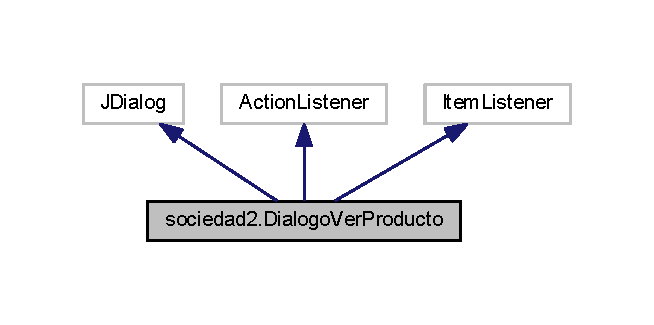
\includegraphics[width=314pt]{classsociedad2_1_1_dialogo_ver_producto__inherit__graph}
\end{center}
\end{figure}


Collaboration diagram for sociedad2.\+Dialogo\+Ver\+Producto\+:
\nopagebreak
\begin{figure}[H]
\begin{center}
\leavevmode
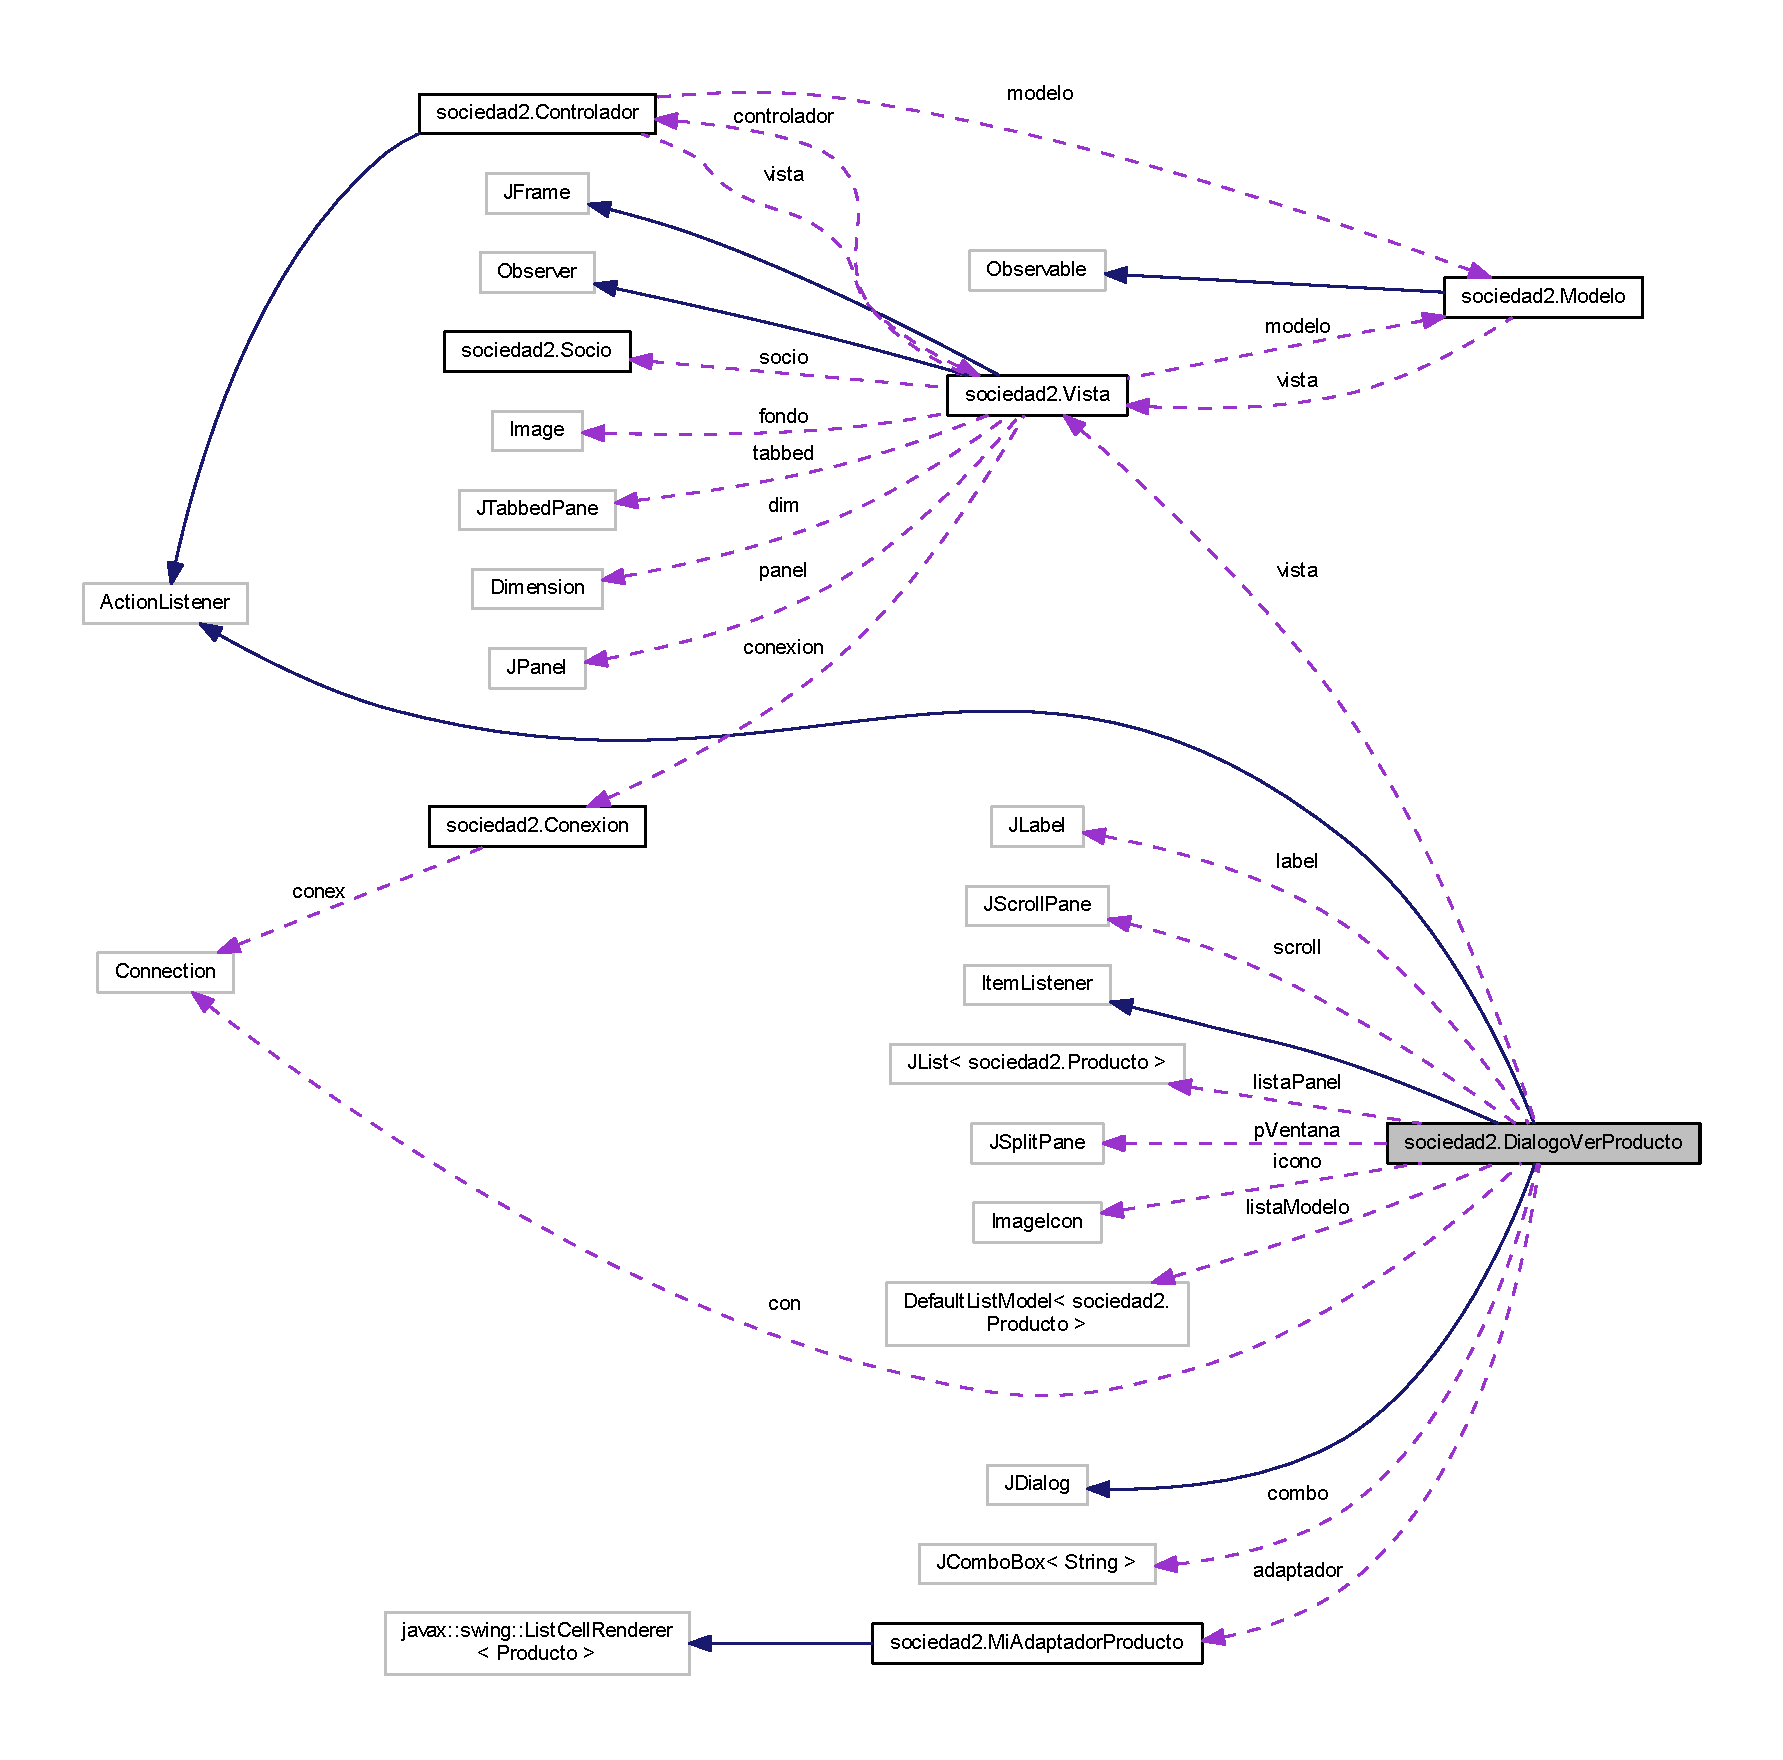
\includegraphics[width=350pt]{classsociedad2_1_1_dialogo_ver_producto__coll__graph}
\end{center}
\end{figure}
\subsection*{Public Member Functions}
\begin{DoxyCompactItemize}
\item 
\mbox{\hyperlink{classsociedad2_1_1_dialogo_ver_producto_a487e0e9d7f6d8b34c62c77920e1db317}{Dialogo\+Ver\+Producto}} (\mbox{\hyperlink{classsociedad2_1_1_vista}{Vista}} vista, String comando, String info, Connection con)  throws S\+Q\+L\+Exception 
\item 
Component \mbox{\hyperlink{classsociedad2_1_1_dialogo_ver_producto_a14b7bf28144868d348c11cc781362b33}{crear\+Panel\+Scroll}} ()  throws S\+Q\+L\+Exception 
\item 
Container \mbox{\hyperlink{classsociedad2_1_1_dialogo_ver_producto_a614453b9afc5ce8151080134d1fe9ee9}{crear\+Botones}} (String titulo)
\item 
Container \mbox{\hyperlink{classsociedad2_1_1_dialogo_ver_producto_a38490a666f21e0b4656d42d3e2e0d56f}{crear\+Panel\+Botones}} ()
\item 
Array\+List$<$ \mbox{\hyperlink{classsociedad2_1_1_producto}{Producto}} $>$ \mbox{\hyperlink{classsociedad2_1_1_dialogo_ver_producto_a4de5041f6b98f27067d84875d96740ad}{Info\+Producto}} (String comando, String info, Connection con)  throws S\+Q\+L\+Exception 
\item 
void \mbox{\hyperlink{classsociedad2_1_1_dialogo_ver_producto_a5e631781eea3e411d84f9d4b61c51d99}{action\+Performed}} (Action\+Event e)
\item 
void \mbox{\hyperlink{classsociedad2_1_1_dialogo_ver_producto_a9c92fe26ec107a5105fe32f9a51c7502}{item\+State\+Changed}} (Item\+Event e)
\end{DoxyCompactItemize}


\subsection{Detailed Description}


Definition at line 34 of file Dialogo\+Ver\+Producto.\+java.



\subsection{Constructor \& Destructor Documentation}
\mbox{\Hypertarget{classsociedad2_1_1_dialogo_ver_producto_a487e0e9d7f6d8b34c62c77920e1db317}\label{classsociedad2_1_1_dialogo_ver_producto_a487e0e9d7f6d8b34c62c77920e1db317}} 
\index{sociedad2\+::\+Dialogo\+Ver\+Producto@{sociedad2\+::\+Dialogo\+Ver\+Producto}!Dialogo\+Ver\+Producto@{Dialogo\+Ver\+Producto}}
\index{Dialogo\+Ver\+Producto@{Dialogo\+Ver\+Producto}!sociedad2\+::\+Dialogo\+Ver\+Producto@{sociedad2\+::\+Dialogo\+Ver\+Producto}}
\subsubsection{\texorpdfstring{Dialogo\+Ver\+Producto()}{DialogoVerProducto()}}
{\footnotesize\ttfamily sociedad2.\+Dialogo\+Ver\+Producto.\+Dialogo\+Ver\+Producto (\begin{DoxyParamCaption}\item[{\mbox{\hyperlink{classsociedad2_1_1_vista}{Vista}}}]{vista,  }\item[{String}]{comando,  }\item[{String}]{info,  }\item[{Connection}]{con }\end{DoxyParamCaption}) throws S\+Q\+L\+Exception}



Definition at line 48 of file Dialogo\+Ver\+Producto.\+java.



\subsection{Member Function Documentation}
\mbox{\Hypertarget{classsociedad2_1_1_dialogo_ver_producto_a5e631781eea3e411d84f9d4b61c51d99}\label{classsociedad2_1_1_dialogo_ver_producto_a5e631781eea3e411d84f9d4b61c51d99}} 
\index{sociedad2\+::\+Dialogo\+Ver\+Producto@{sociedad2\+::\+Dialogo\+Ver\+Producto}!action\+Performed@{action\+Performed}}
\index{action\+Performed@{action\+Performed}!sociedad2\+::\+Dialogo\+Ver\+Producto@{sociedad2\+::\+Dialogo\+Ver\+Producto}}
\subsubsection{\texorpdfstring{action\+Performed()}{actionPerformed()}}
{\footnotesize\ttfamily void sociedad2.\+Dialogo\+Ver\+Producto.\+action\+Performed (\begin{DoxyParamCaption}\item[{Action\+Event}]{e }\end{DoxyParamCaption})}



Definition at line 204 of file Dialogo\+Ver\+Producto.\+java.

\mbox{\Hypertarget{classsociedad2_1_1_dialogo_ver_producto_a614453b9afc5ce8151080134d1fe9ee9}\label{classsociedad2_1_1_dialogo_ver_producto_a614453b9afc5ce8151080134d1fe9ee9}} 
\index{sociedad2\+::\+Dialogo\+Ver\+Producto@{sociedad2\+::\+Dialogo\+Ver\+Producto}!crear\+Botones@{crear\+Botones}}
\index{crear\+Botones@{crear\+Botones}!sociedad2\+::\+Dialogo\+Ver\+Producto@{sociedad2\+::\+Dialogo\+Ver\+Producto}}
\subsubsection{\texorpdfstring{crear\+Botones()}{crearBotones()}}
{\footnotesize\ttfamily Container sociedad2.\+Dialogo\+Ver\+Producto.\+crear\+Botones (\begin{DoxyParamCaption}\item[{String}]{titulo }\end{DoxyParamCaption})}



Definition at line 121 of file Dialogo\+Ver\+Producto.\+java.

\mbox{\Hypertarget{classsociedad2_1_1_dialogo_ver_producto_a38490a666f21e0b4656d42d3e2e0d56f}\label{classsociedad2_1_1_dialogo_ver_producto_a38490a666f21e0b4656d42d3e2e0d56f}} 
\index{sociedad2\+::\+Dialogo\+Ver\+Producto@{sociedad2\+::\+Dialogo\+Ver\+Producto}!crear\+Panel\+Botones@{crear\+Panel\+Botones}}
\index{crear\+Panel\+Botones@{crear\+Panel\+Botones}!sociedad2\+::\+Dialogo\+Ver\+Producto@{sociedad2\+::\+Dialogo\+Ver\+Producto}}
\subsubsection{\texorpdfstring{crear\+Panel\+Botones()}{crearPanelBotones()}}
{\footnotesize\ttfamily Container sociedad2.\+Dialogo\+Ver\+Producto.\+crear\+Panel\+Botones (\begin{DoxyParamCaption}{ }\end{DoxyParamCaption})}



Definition at line 130 of file Dialogo\+Ver\+Producto.\+java.

\mbox{\Hypertarget{classsociedad2_1_1_dialogo_ver_producto_a14b7bf28144868d348c11cc781362b33}\label{classsociedad2_1_1_dialogo_ver_producto_a14b7bf28144868d348c11cc781362b33}} 
\index{sociedad2\+::\+Dialogo\+Ver\+Producto@{sociedad2\+::\+Dialogo\+Ver\+Producto}!crear\+Panel\+Scroll@{crear\+Panel\+Scroll}}
\index{crear\+Panel\+Scroll@{crear\+Panel\+Scroll}!sociedad2\+::\+Dialogo\+Ver\+Producto@{sociedad2\+::\+Dialogo\+Ver\+Producto}}
\subsubsection{\texorpdfstring{crear\+Panel\+Scroll()}{crearPanelScroll()}}
{\footnotesize\ttfamily Component sociedad2.\+Dialogo\+Ver\+Producto.\+crear\+Panel\+Scroll (\begin{DoxyParamCaption}{ }\end{DoxyParamCaption}) throws S\+Q\+L\+Exception}



Definition at line 80 of file Dialogo\+Ver\+Producto.\+java.

\mbox{\Hypertarget{classsociedad2_1_1_dialogo_ver_producto_a4de5041f6b98f27067d84875d96740ad}\label{classsociedad2_1_1_dialogo_ver_producto_a4de5041f6b98f27067d84875d96740ad}} 
\index{sociedad2\+::\+Dialogo\+Ver\+Producto@{sociedad2\+::\+Dialogo\+Ver\+Producto}!Info\+Producto@{Info\+Producto}}
\index{Info\+Producto@{Info\+Producto}!sociedad2\+::\+Dialogo\+Ver\+Producto@{sociedad2\+::\+Dialogo\+Ver\+Producto}}
\subsubsection{\texorpdfstring{Info\+Producto()}{InfoProducto()}}
{\footnotesize\ttfamily Array\+List$<$\mbox{\hyperlink{classsociedad2_1_1_producto}{Producto}}$>$ sociedad2.\+Dialogo\+Ver\+Producto.\+Info\+Producto (\begin{DoxyParamCaption}\item[{String}]{comando,  }\item[{String}]{info,  }\item[{Connection}]{con }\end{DoxyParamCaption}) throws S\+Q\+L\+Exception}



Definition at line 142 of file Dialogo\+Ver\+Producto.\+java.

\mbox{\Hypertarget{classsociedad2_1_1_dialogo_ver_producto_a9c92fe26ec107a5105fe32f9a51c7502}\label{classsociedad2_1_1_dialogo_ver_producto_a9c92fe26ec107a5105fe32f9a51c7502}} 
\index{sociedad2\+::\+Dialogo\+Ver\+Producto@{sociedad2\+::\+Dialogo\+Ver\+Producto}!item\+State\+Changed@{item\+State\+Changed}}
\index{item\+State\+Changed@{item\+State\+Changed}!sociedad2\+::\+Dialogo\+Ver\+Producto@{sociedad2\+::\+Dialogo\+Ver\+Producto}}
\subsubsection{\texorpdfstring{item\+State\+Changed()}{itemStateChanged()}}
{\footnotesize\ttfamily void sociedad2.\+Dialogo\+Ver\+Producto.\+item\+State\+Changed (\begin{DoxyParamCaption}\item[{Item\+Event}]{e }\end{DoxyParamCaption})}



Definition at line 251 of file Dialogo\+Ver\+Producto.\+java.



The documentation for this class was generated from the following file\+:\begin{DoxyCompactItemize}
\item 
E\+:/eclipse-\/workspace/\+Sociedad/src/sociedad2/\mbox{\hyperlink{_dialogo_ver_producto_8java}{Dialogo\+Ver\+Producto.\+java}}\end{DoxyCompactItemize}

\hypertarget{classsociedad2_1_1_dialogo_ver_productos_baja}{}\section{sociedad2.\+Dialogo\+Ver\+Productos\+Baja Class Reference}
\label{classsociedad2_1_1_dialogo_ver_productos_baja}\index{sociedad2.\+Dialogo\+Ver\+Productos\+Baja@{sociedad2.\+Dialogo\+Ver\+Productos\+Baja}}


Inheritance diagram for sociedad2.\+Dialogo\+Ver\+Productos\+Baja\+:\nopagebreak
\begin{figure}[H]
\begin{center}
\leavevmode
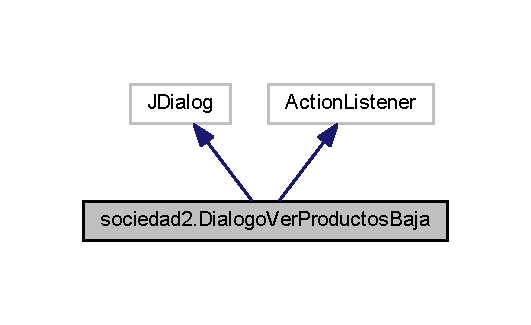
\includegraphics[width=255pt]{classsociedad2_1_1_dialogo_ver_productos_baja__inherit__graph}
\end{center}
\end{figure}


Collaboration diagram for sociedad2.\+Dialogo\+Ver\+Productos\+Baja\+:
\nopagebreak
\begin{figure}[H]
\begin{center}
\leavevmode
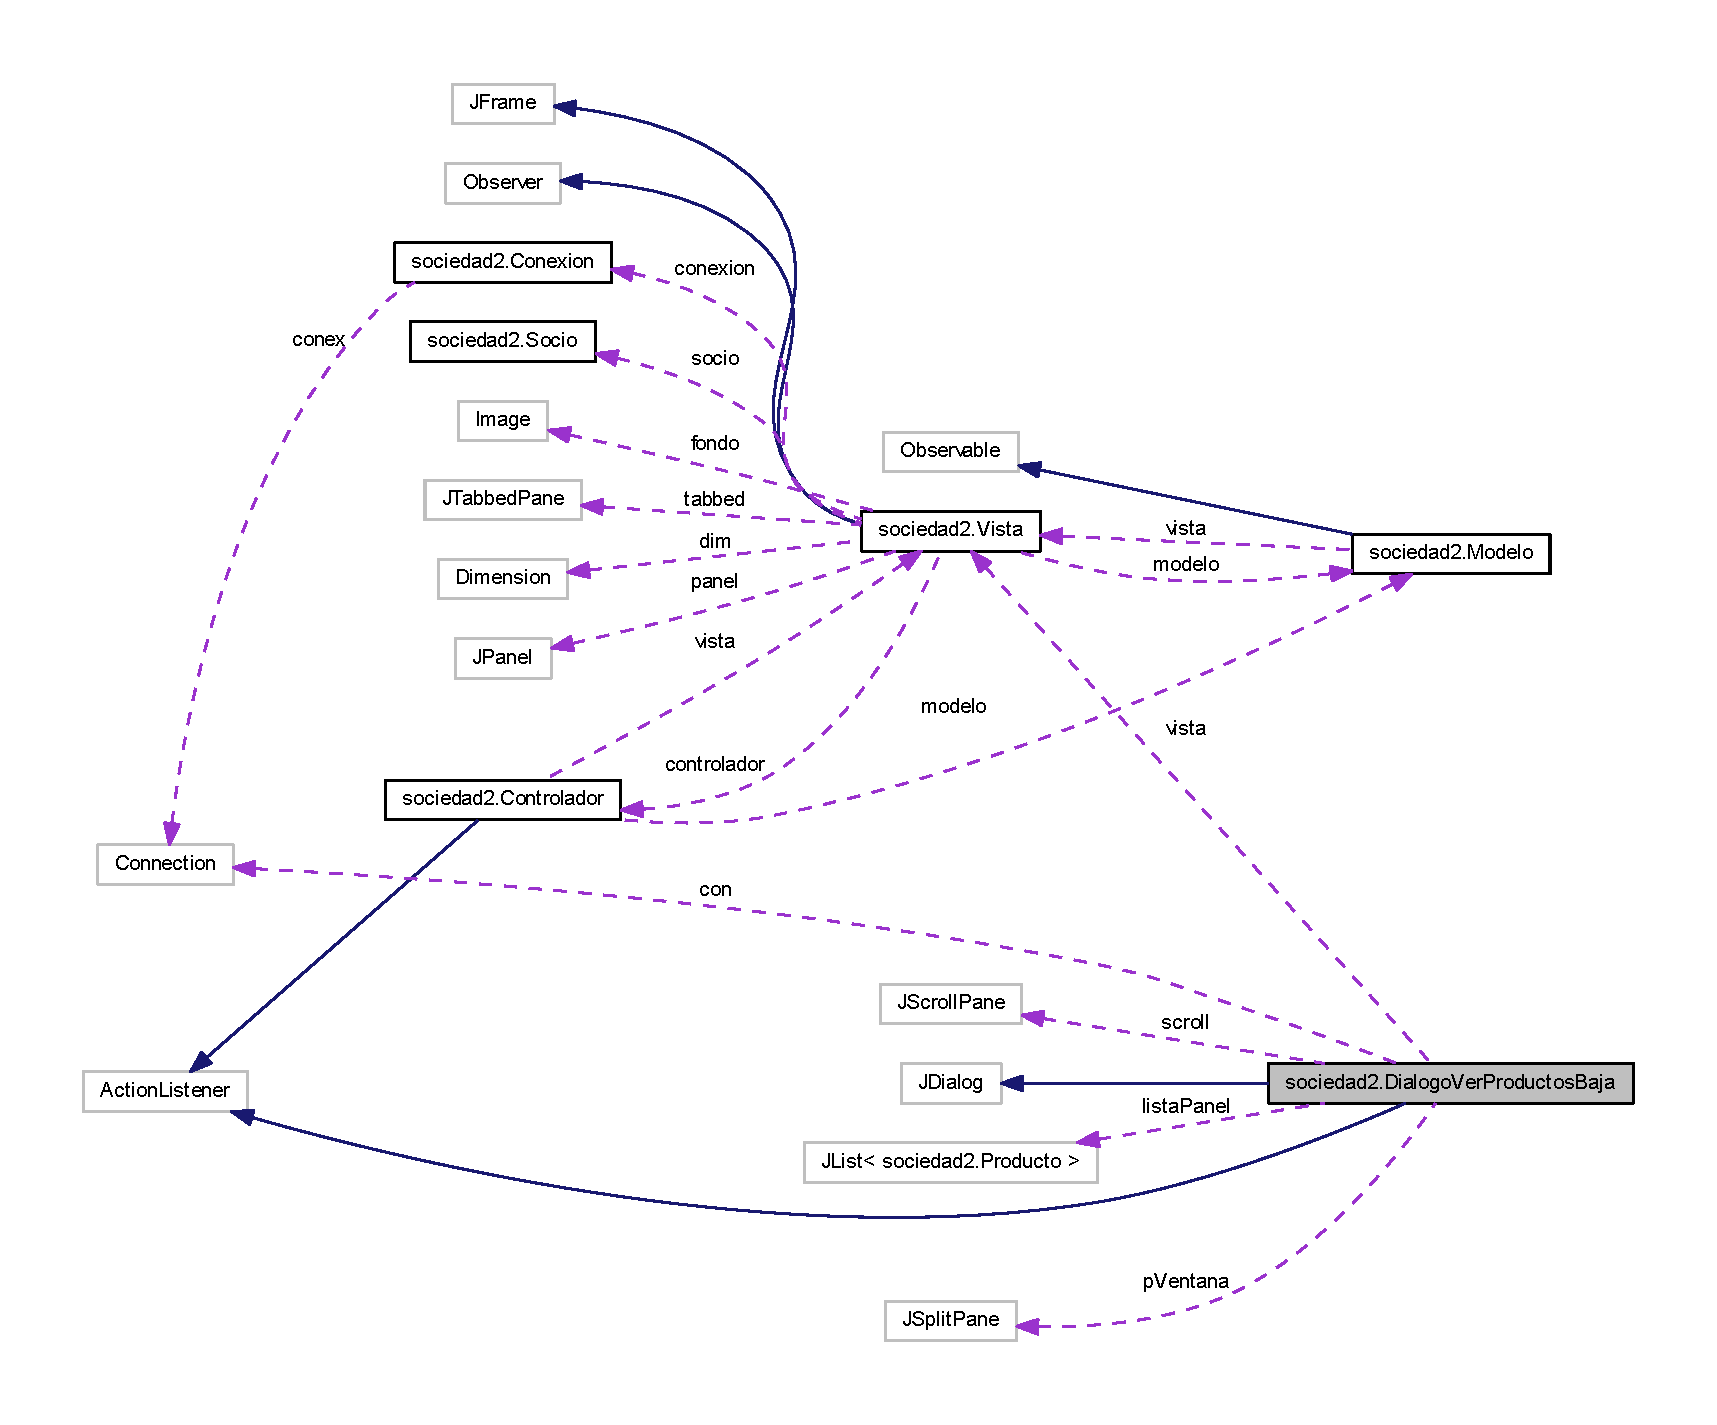
\includegraphics[width=350pt]{classsociedad2_1_1_dialogo_ver_productos_baja__coll__graph}
\end{center}
\end{figure}
\subsection*{Public Member Functions}
\begin{DoxyCompactItemize}
\item 
\mbox{\hyperlink{classsociedad2_1_1_dialogo_ver_productos_baja_a9655028d797c1cb985341f22903bc366}{Dialogo\+Ver\+Productos\+Baja}} (\mbox{\hyperlink{classsociedad2_1_1_vista}{Vista}} vista, String comando, String info, Connection con)  throws S\+Q\+L\+Exception 
\item 
Array\+List$<$ \mbox{\hyperlink{classsociedad2_1_1_producto}{Producto}} $>$ \mbox{\hyperlink{classsociedad2_1_1_dialogo_ver_productos_baja_a3cebb225abaf25d0171deedb0fc7dab4}{Info\+Productos}} (String comando, String info, Connection con)  throws S\+Q\+L\+Exception 
\item 
Container \mbox{\hyperlink{classsociedad2_1_1_dialogo_ver_productos_baja_a9a5c2029fed8b8593bf5331a4839cf9b}{crear\+Botones}} (String titulo)
\item 
Container \mbox{\hyperlink{classsociedad2_1_1_dialogo_ver_productos_baja_a7485030e445c2915f90b38075dddb5a3}{crear\+Panel\+Botones}} (int id)
\item 
void \mbox{\hyperlink{classsociedad2_1_1_dialogo_ver_productos_baja_a039af7e6be4890ca43497d8922c30df7}{action\+Performed}} (Action\+Event e)
\end{DoxyCompactItemize}


\subsection{Detailed Description}


Definition at line 21 of file Dialogo\+Ver\+Productos\+Baja.\+java.



\subsection{Constructor \& Destructor Documentation}
\mbox{\Hypertarget{classsociedad2_1_1_dialogo_ver_productos_baja_a9655028d797c1cb985341f22903bc366}\label{classsociedad2_1_1_dialogo_ver_productos_baja_a9655028d797c1cb985341f22903bc366}} 
\index{sociedad2\+::\+Dialogo\+Ver\+Productos\+Baja@{sociedad2\+::\+Dialogo\+Ver\+Productos\+Baja}!Dialogo\+Ver\+Productos\+Baja@{Dialogo\+Ver\+Productos\+Baja}}
\index{Dialogo\+Ver\+Productos\+Baja@{Dialogo\+Ver\+Productos\+Baja}!sociedad2\+::\+Dialogo\+Ver\+Productos\+Baja@{sociedad2\+::\+Dialogo\+Ver\+Productos\+Baja}}
\subsubsection{\texorpdfstring{Dialogo\+Ver\+Productos\+Baja()}{DialogoVerProductosBaja()}}
{\footnotesize\ttfamily sociedad2.\+Dialogo\+Ver\+Productos\+Baja.\+Dialogo\+Ver\+Productos\+Baja (\begin{DoxyParamCaption}\item[{\mbox{\hyperlink{classsociedad2_1_1_vista}{Vista}}}]{vista,  }\item[{String}]{comando,  }\item[{String}]{info,  }\item[{Connection}]{con }\end{DoxyParamCaption}) throws S\+Q\+L\+Exception}



Definition at line 31 of file Dialogo\+Ver\+Productos\+Baja.\+java.



\subsection{Member Function Documentation}
\mbox{\Hypertarget{classsociedad2_1_1_dialogo_ver_productos_baja_a039af7e6be4890ca43497d8922c30df7}\label{classsociedad2_1_1_dialogo_ver_productos_baja_a039af7e6be4890ca43497d8922c30df7}} 
\index{sociedad2\+::\+Dialogo\+Ver\+Productos\+Baja@{sociedad2\+::\+Dialogo\+Ver\+Productos\+Baja}!action\+Performed@{action\+Performed}}
\index{action\+Performed@{action\+Performed}!sociedad2\+::\+Dialogo\+Ver\+Productos\+Baja@{sociedad2\+::\+Dialogo\+Ver\+Productos\+Baja}}
\subsubsection{\texorpdfstring{action\+Performed()}{actionPerformed()}}
{\footnotesize\ttfamily void sociedad2.\+Dialogo\+Ver\+Productos\+Baja.\+action\+Performed (\begin{DoxyParamCaption}\item[{Action\+Event}]{e }\end{DoxyParamCaption})}



Definition at line 104 of file Dialogo\+Ver\+Productos\+Baja.\+java.

\mbox{\Hypertarget{classsociedad2_1_1_dialogo_ver_productos_baja_a9a5c2029fed8b8593bf5331a4839cf9b}\label{classsociedad2_1_1_dialogo_ver_productos_baja_a9a5c2029fed8b8593bf5331a4839cf9b}} 
\index{sociedad2\+::\+Dialogo\+Ver\+Productos\+Baja@{sociedad2\+::\+Dialogo\+Ver\+Productos\+Baja}!crear\+Botones@{crear\+Botones}}
\index{crear\+Botones@{crear\+Botones}!sociedad2\+::\+Dialogo\+Ver\+Productos\+Baja@{sociedad2\+::\+Dialogo\+Ver\+Productos\+Baja}}
\subsubsection{\texorpdfstring{crear\+Botones()}{crearBotones()}}
{\footnotesize\ttfamily Container sociedad2.\+Dialogo\+Ver\+Productos\+Baja.\+crear\+Botones (\begin{DoxyParamCaption}\item[{String}]{titulo }\end{DoxyParamCaption})}



Definition at line 84 of file Dialogo\+Ver\+Productos\+Baja.\+java.

\mbox{\Hypertarget{classsociedad2_1_1_dialogo_ver_productos_baja_a7485030e445c2915f90b38075dddb5a3}\label{classsociedad2_1_1_dialogo_ver_productos_baja_a7485030e445c2915f90b38075dddb5a3}} 
\index{sociedad2\+::\+Dialogo\+Ver\+Productos\+Baja@{sociedad2\+::\+Dialogo\+Ver\+Productos\+Baja}!crear\+Panel\+Botones@{crear\+Panel\+Botones}}
\index{crear\+Panel\+Botones@{crear\+Panel\+Botones}!sociedad2\+::\+Dialogo\+Ver\+Productos\+Baja@{sociedad2\+::\+Dialogo\+Ver\+Productos\+Baja}}
\subsubsection{\texorpdfstring{crear\+Panel\+Botones()}{crearPanelBotones()}}
{\footnotesize\ttfamily Container sociedad2.\+Dialogo\+Ver\+Productos\+Baja.\+crear\+Panel\+Botones (\begin{DoxyParamCaption}\item[{int}]{id }\end{DoxyParamCaption})}



Definition at line 93 of file Dialogo\+Ver\+Productos\+Baja.\+java.

\mbox{\Hypertarget{classsociedad2_1_1_dialogo_ver_productos_baja_a3cebb225abaf25d0171deedb0fc7dab4}\label{classsociedad2_1_1_dialogo_ver_productos_baja_a3cebb225abaf25d0171deedb0fc7dab4}} 
\index{sociedad2\+::\+Dialogo\+Ver\+Productos\+Baja@{sociedad2\+::\+Dialogo\+Ver\+Productos\+Baja}!Info\+Productos@{Info\+Productos}}
\index{Info\+Productos@{Info\+Productos}!sociedad2\+::\+Dialogo\+Ver\+Productos\+Baja@{sociedad2\+::\+Dialogo\+Ver\+Productos\+Baja}}
\subsubsection{\texorpdfstring{Info\+Productos()}{InfoProductos()}}
{\footnotesize\ttfamily Array\+List$<$\mbox{\hyperlink{classsociedad2_1_1_producto}{Producto}}$>$ sociedad2.\+Dialogo\+Ver\+Productos\+Baja.\+Info\+Productos (\begin{DoxyParamCaption}\item[{String}]{comando,  }\item[{String}]{info,  }\item[{Connection}]{con }\end{DoxyParamCaption}) throws S\+Q\+L\+Exception}



Definition at line 76 of file Dialogo\+Ver\+Productos\+Baja.\+java.



The documentation for this class was generated from the following file\+:\begin{DoxyCompactItemize}
\item 
E\+:/eclipse-\/workspace/\+Sociedad/src/sociedad2/\mbox{\hyperlink{_dialogo_ver_productos_baja_8java}{Dialogo\+Ver\+Productos\+Baja.\+java}}\end{DoxyCompactItemize}

\hypertarget{classsociedad2_1_1_dialogo_ver_socio}{}\section{sociedad2.\+Dialogo\+Ver\+Socio Class Reference}
\label{classsociedad2_1_1_dialogo_ver_socio}\index{sociedad2.\+Dialogo\+Ver\+Socio@{sociedad2.\+Dialogo\+Ver\+Socio}}


Inheritance diagram for sociedad2.\+Dialogo\+Ver\+Socio\+:\nopagebreak
\begin{figure}[H]
\begin{center}
\leavevmode
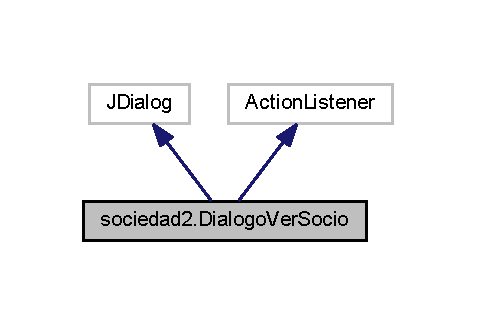
\includegraphics[width=229pt]{classsociedad2_1_1_dialogo_ver_socio__inherit__graph}
\end{center}
\end{figure}


Collaboration diagram for sociedad2.\+Dialogo\+Ver\+Socio\+:
\nopagebreak
\begin{figure}[H]
\begin{center}
\leavevmode
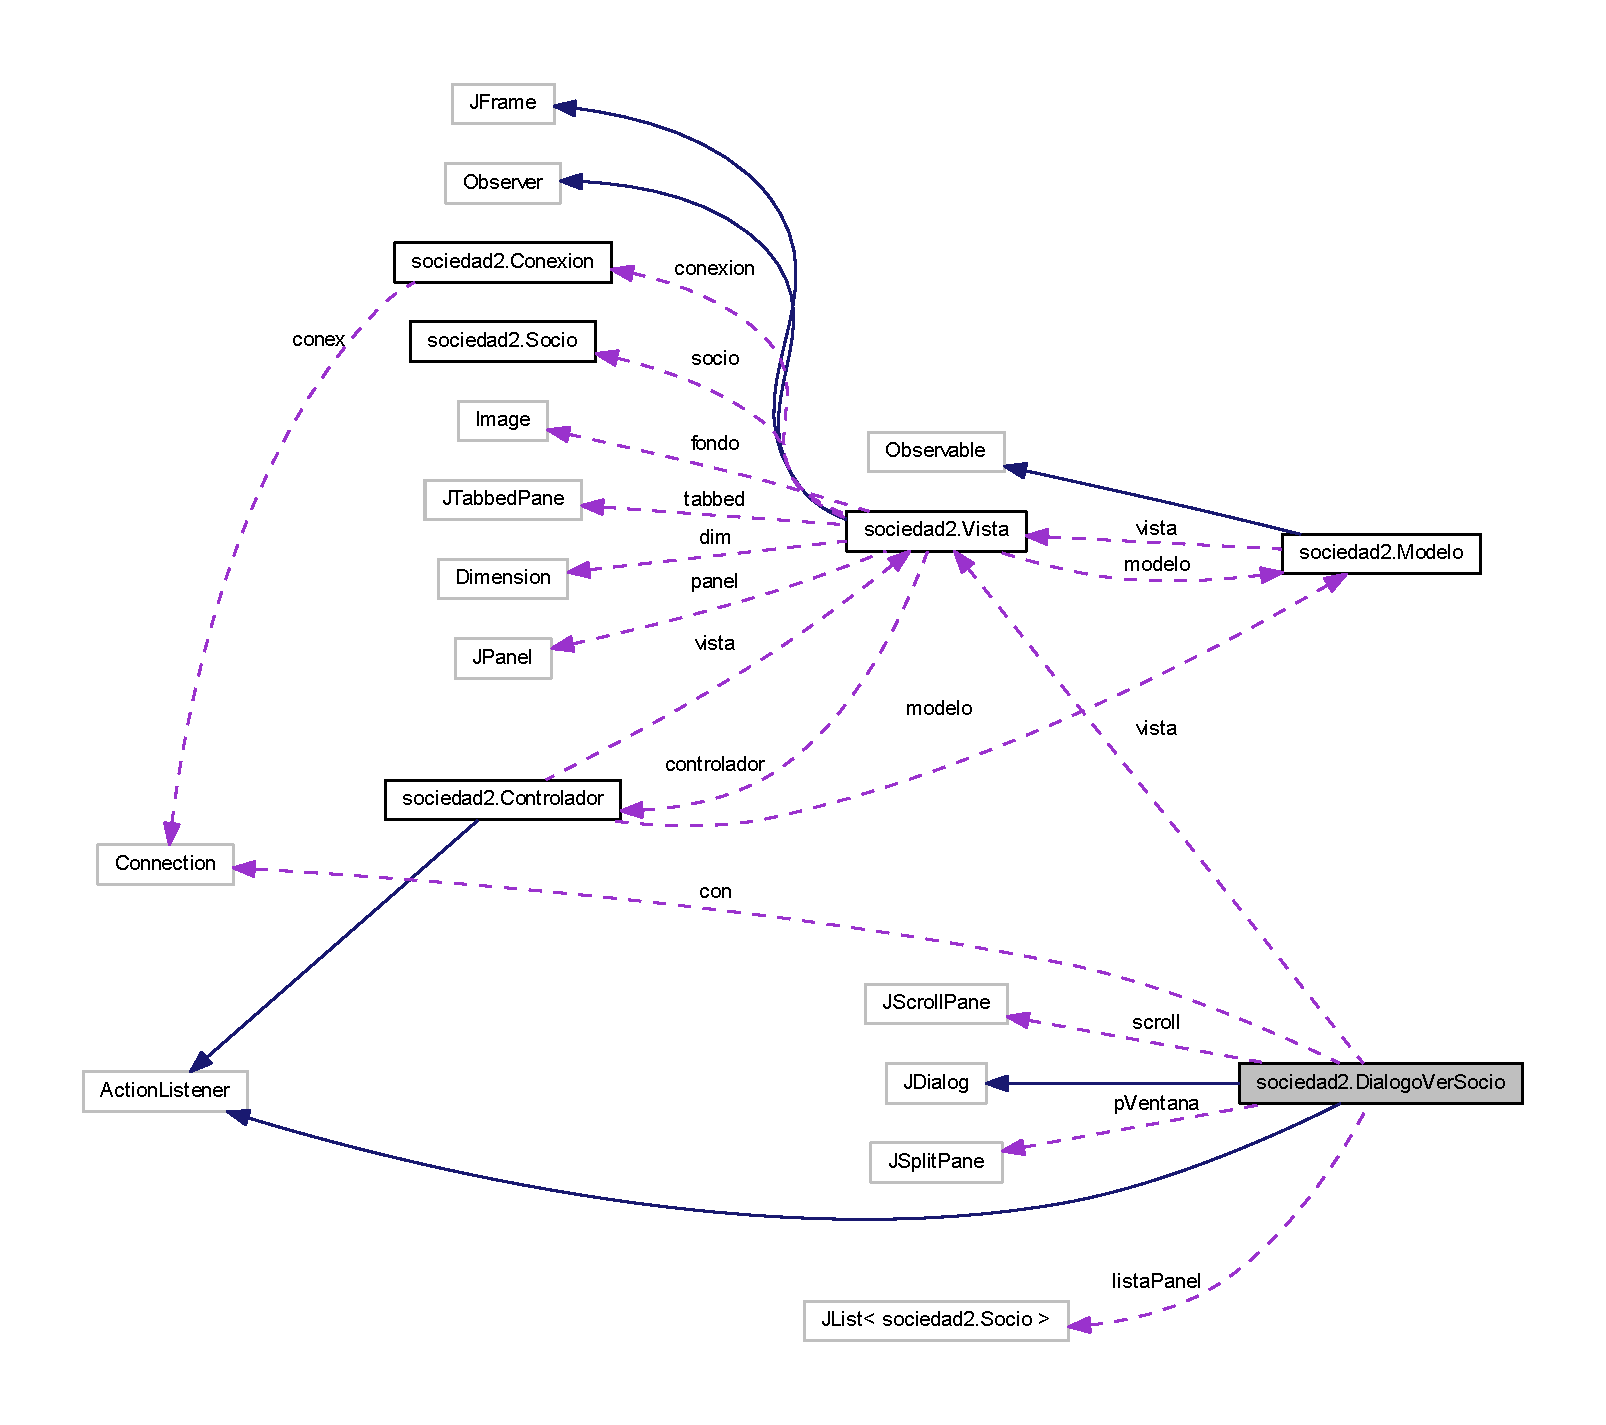
\includegraphics[width=350pt]{classsociedad2_1_1_dialogo_ver_socio__coll__graph}
\end{center}
\end{figure}
\subsection*{Public Member Functions}
\begin{DoxyCompactItemize}
\item 
\mbox{\hyperlink{classsociedad2_1_1_dialogo_ver_socio_ab4314628e90ec29d1985716a5e1cecda}{Dialogo\+Ver\+Socio}} (\mbox{\hyperlink{classsociedad2_1_1_vista}{Vista}} vista, String comando, String info, Connection con)  throws S\+Q\+L\+Exception 
\item 
Array\+List$<$ \mbox{\hyperlink{classsociedad2_1_1_socio}{Socio}} $>$ \mbox{\hyperlink{classsociedad2_1_1_dialogo_ver_socio_aa6ecfb71916851860dd14056bc201f11}{Info\+Socios}} (String comando, String info, Connection con)  throws S\+Q\+L\+Exception 
\item 
Container \mbox{\hyperlink{classsociedad2_1_1_dialogo_ver_socio_ac6fc8788c34fb7f99282d5aa6ff43a4d}{crear\+Botones}} (String titulo)
\item 
Container \mbox{\hyperlink{classsociedad2_1_1_dialogo_ver_socio_a7ee9729c4602fe14eda688a29d56a28f}{crear\+Panel\+Botones}} ()
\item 
void \mbox{\hyperlink{classsociedad2_1_1_dialogo_ver_socio_a0e948f9ccbacd50e3464bd87fd13b82d}{action\+Performed}} (Action\+Event e)
\end{DoxyCompactItemize}


\subsection{Detailed Description}


Definition at line 28 of file Dialogo\+Ver\+Socio.\+java.



\subsection{Constructor \& Destructor Documentation}
\mbox{\Hypertarget{classsociedad2_1_1_dialogo_ver_socio_ab4314628e90ec29d1985716a5e1cecda}\label{classsociedad2_1_1_dialogo_ver_socio_ab4314628e90ec29d1985716a5e1cecda}} 
\index{sociedad2\+::\+Dialogo\+Ver\+Socio@{sociedad2\+::\+Dialogo\+Ver\+Socio}!Dialogo\+Ver\+Socio@{Dialogo\+Ver\+Socio}}
\index{Dialogo\+Ver\+Socio@{Dialogo\+Ver\+Socio}!sociedad2\+::\+Dialogo\+Ver\+Socio@{sociedad2\+::\+Dialogo\+Ver\+Socio}}
\subsubsection{\texorpdfstring{Dialogo\+Ver\+Socio()}{DialogoVerSocio()}}
{\footnotesize\ttfamily sociedad2.\+Dialogo\+Ver\+Socio.\+Dialogo\+Ver\+Socio (\begin{DoxyParamCaption}\item[{\mbox{\hyperlink{classsociedad2_1_1_vista}{Vista}}}]{vista,  }\item[{String}]{comando,  }\item[{String}]{info,  }\item[{Connection}]{con }\end{DoxyParamCaption}) throws S\+Q\+L\+Exception}



Definition at line 38 of file Dialogo\+Ver\+Socio.\+java.



\subsection{Member Function Documentation}
\mbox{\Hypertarget{classsociedad2_1_1_dialogo_ver_socio_a0e948f9ccbacd50e3464bd87fd13b82d}\label{classsociedad2_1_1_dialogo_ver_socio_a0e948f9ccbacd50e3464bd87fd13b82d}} 
\index{sociedad2\+::\+Dialogo\+Ver\+Socio@{sociedad2\+::\+Dialogo\+Ver\+Socio}!action\+Performed@{action\+Performed}}
\index{action\+Performed@{action\+Performed}!sociedad2\+::\+Dialogo\+Ver\+Socio@{sociedad2\+::\+Dialogo\+Ver\+Socio}}
\subsubsection{\texorpdfstring{action\+Performed()}{actionPerformed()}}
{\footnotesize\ttfamily void sociedad2.\+Dialogo\+Ver\+Socio.\+action\+Performed (\begin{DoxyParamCaption}\item[{Action\+Event}]{e }\end{DoxyParamCaption})}



Definition at line 111 of file Dialogo\+Ver\+Socio.\+java.

\mbox{\Hypertarget{classsociedad2_1_1_dialogo_ver_socio_ac6fc8788c34fb7f99282d5aa6ff43a4d}\label{classsociedad2_1_1_dialogo_ver_socio_ac6fc8788c34fb7f99282d5aa6ff43a4d}} 
\index{sociedad2\+::\+Dialogo\+Ver\+Socio@{sociedad2\+::\+Dialogo\+Ver\+Socio}!crear\+Botones@{crear\+Botones}}
\index{crear\+Botones@{crear\+Botones}!sociedad2\+::\+Dialogo\+Ver\+Socio@{sociedad2\+::\+Dialogo\+Ver\+Socio}}
\subsubsection{\texorpdfstring{crear\+Botones()}{crearBotones()}}
{\footnotesize\ttfamily Container sociedad2.\+Dialogo\+Ver\+Socio.\+crear\+Botones (\begin{DoxyParamCaption}\item[{String}]{titulo }\end{DoxyParamCaption})}



Definition at line 91 of file Dialogo\+Ver\+Socio.\+java.

\mbox{\Hypertarget{classsociedad2_1_1_dialogo_ver_socio_a7ee9729c4602fe14eda688a29d56a28f}\label{classsociedad2_1_1_dialogo_ver_socio_a7ee9729c4602fe14eda688a29d56a28f}} 
\index{sociedad2\+::\+Dialogo\+Ver\+Socio@{sociedad2\+::\+Dialogo\+Ver\+Socio}!crear\+Panel\+Botones@{crear\+Panel\+Botones}}
\index{crear\+Panel\+Botones@{crear\+Panel\+Botones}!sociedad2\+::\+Dialogo\+Ver\+Socio@{sociedad2\+::\+Dialogo\+Ver\+Socio}}
\subsubsection{\texorpdfstring{crear\+Panel\+Botones()}{crearPanelBotones()}}
{\footnotesize\ttfamily Container sociedad2.\+Dialogo\+Ver\+Socio.\+crear\+Panel\+Botones (\begin{DoxyParamCaption}{ }\end{DoxyParamCaption})}



Definition at line 100 of file Dialogo\+Ver\+Socio.\+java.

\mbox{\Hypertarget{classsociedad2_1_1_dialogo_ver_socio_aa6ecfb71916851860dd14056bc201f11}\label{classsociedad2_1_1_dialogo_ver_socio_aa6ecfb71916851860dd14056bc201f11}} 
\index{sociedad2\+::\+Dialogo\+Ver\+Socio@{sociedad2\+::\+Dialogo\+Ver\+Socio}!Info\+Socios@{Info\+Socios}}
\index{Info\+Socios@{Info\+Socios}!sociedad2\+::\+Dialogo\+Ver\+Socio@{sociedad2\+::\+Dialogo\+Ver\+Socio}}
\subsubsection{\texorpdfstring{Info\+Socios()}{InfoSocios()}}
{\footnotesize\ttfamily Array\+List$<$\mbox{\hyperlink{classsociedad2_1_1_socio}{Socio}}$>$ sociedad2.\+Dialogo\+Ver\+Socio.\+Info\+Socios (\begin{DoxyParamCaption}\item[{String}]{comando,  }\item[{String}]{info,  }\item[{Connection}]{con }\end{DoxyParamCaption}) throws S\+Q\+L\+Exception}



Definition at line 83 of file Dialogo\+Ver\+Socio.\+java.



The documentation for this class was generated from the following file\+:\begin{DoxyCompactItemize}
\item 
E\+:/eclipse-\/workspace/\+Sociedad/src/sociedad2/\mbox{\hyperlink{_dialogo_ver_socio_8java}{Dialogo\+Ver\+Socio.\+java}}\end{DoxyCompactItemize}

\hypertarget{classsociedad2_1_1_dialogo_ver_socios_baja}{}\section{sociedad2.\+Dialogo\+Ver\+Socios\+Baja Class Reference}
\label{classsociedad2_1_1_dialogo_ver_socios_baja}\index{sociedad2.\+Dialogo\+Ver\+Socios\+Baja@{sociedad2.\+Dialogo\+Ver\+Socios\+Baja}}


Inheritance diagram for sociedad2.\+Dialogo\+Ver\+Socios\+Baja\+:
\nopagebreak
\begin{figure}[H]
\begin{center}
\leavevmode
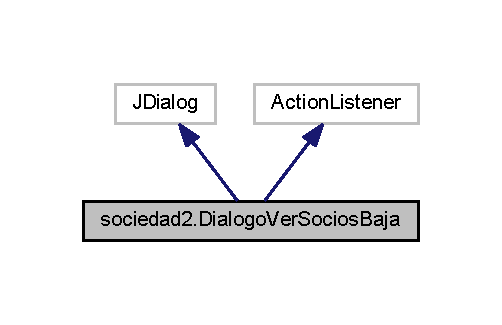
\includegraphics[width=241pt]{classsociedad2_1_1_dialogo_ver_socios_baja__inherit__graph}
\end{center}
\end{figure}


Collaboration diagram for sociedad2.\+Dialogo\+Ver\+Socios\+Baja\+:
\nopagebreak
\begin{figure}[H]
\begin{center}
\leavevmode
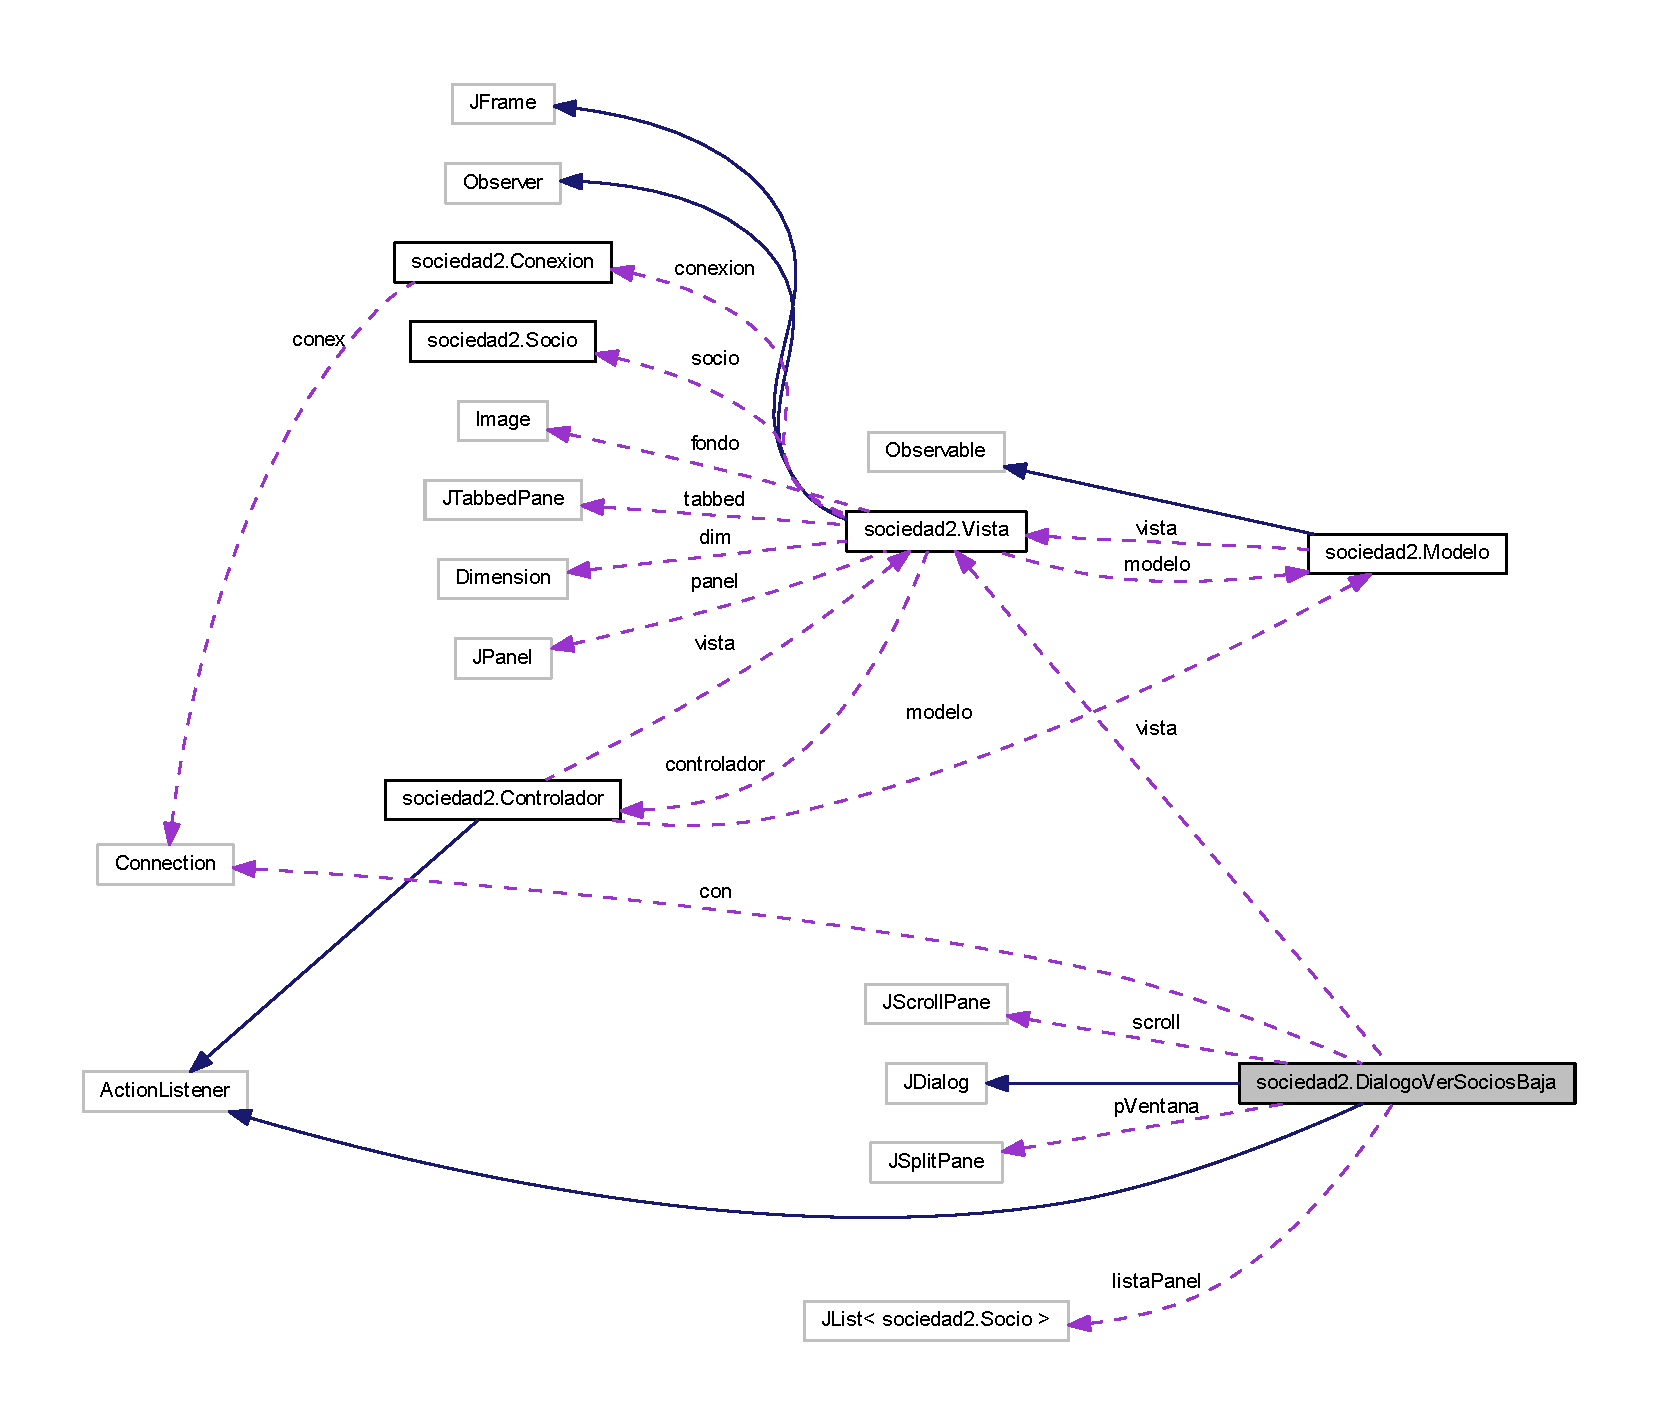
\includegraphics[width=350pt]{classsociedad2_1_1_dialogo_ver_socios_baja__coll__graph}
\end{center}
\end{figure}
\subsection*{Public Member Functions}
\begin{DoxyCompactItemize}
\item 
\mbox{\hyperlink{classsociedad2_1_1_dialogo_ver_socios_baja_a7dd9d7566b4eee0ce8d88b9cfec32600}{Dialogo\+Ver\+Socios\+Baja}} (\mbox{\hyperlink{classsociedad2_1_1_vista}{Vista}} vista, String comando, String info, Connection con)  throws S\+Q\+L\+Exception 
\item 
Array\+List$<$ \mbox{\hyperlink{classsociedad2_1_1_socio}{Socio}} $>$ \mbox{\hyperlink{classsociedad2_1_1_dialogo_ver_socios_baja_a6e73715c1f88a3649f9b524ca781b8e0}{Info\+Socios}} (String comando, String info, Connection con)  throws S\+Q\+L\+Exception 
\item 
Container \mbox{\hyperlink{classsociedad2_1_1_dialogo_ver_socios_baja_a21bf2bac56b7632ec153200d85733c52}{crear\+Botones}} (String titulo)
\item 
Container \mbox{\hyperlink{classsociedad2_1_1_dialogo_ver_socios_baja_a1690764694f81b9b5a5081178fe2ab77}{crear\+Panel\+Botones}} (int id)
\item 
void \mbox{\hyperlink{classsociedad2_1_1_dialogo_ver_socios_baja_abf0650961335d2802e33616ab71fef9e}{action\+Performed}} (Action\+Event e)
\end{DoxyCompactItemize}


\subsection{Detailed Description}


Definition at line 21 of file Dialogo\+Ver\+Socios\+Baja.\+java.



\subsection{Constructor \& Destructor Documentation}
\mbox{\Hypertarget{classsociedad2_1_1_dialogo_ver_socios_baja_a7dd9d7566b4eee0ce8d88b9cfec32600}\label{classsociedad2_1_1_dialogo_ver_socios_baja_a7dd9d7566b4eee0ce8d88b9cfec32600}} 
\index{sociedad2\+::\+Dialogo\+Ver\+Socios\+Baja@{sociedad2\+::\+Dialogo\+Ver\+Socios\+Baja}!Dialogo\+Ver\+Socios\+Baja@{Dialogo\+Ver\+Socios\+Baja}}
\index{Dialogo\+Ver\+Socios\+Baja@{Dialogo\+Ver\+Socios\+Baja}!sociedad2\+::\+Dialogo\+Ver\+Socios\+Baja@{sociedad2\+::\+Dialogo\+Ver\+Socios\+Baja}}
\subsubsection{\texorpdfstring{Dialogo\+Ver\+Socios\+Baja()}{DialogoVerSociosBaja()}}
{\footnotesize\ttfamily sociedad2.\+Dialogo\+Ver\+Socios\+Baja.\+Dialogo\+Ver\+Socios\+Baja (\begin{DoxyParamCaption}\item[{\mbox{\hyperlink{classsociedad2_1_1_vista}{Vista}}}]{vista,  }\item[{String}]{comando,  }\item[{String}]{info,  }\item[{Connection}]{con }\end{DoxyParamCaption}) throws S\+Q\+L\+Exception}



Definition at line 31 of file Dialogo\+Ver\+Socios\+Baja.\+java.



\subsection{Member Function Documentation}
\mbox{\Hypertarget{classsociedad2_1_1_dialogo_ver_socios_baja_abf0650961335d2802e33616ab71fef9e}\label{classsociedad2_1_1_dialogo_ver_socios_baja_abf0650961335d2802e33616ab71fef9e}} 
\index{sociedad2\+::\+Dialogo\+Ver\+Socios\+Baja@{sociedad2\+::\+Dialogo\+Ver\+Socios\+Baja}!action\+Performed@{action\+Performed}}
\index{action\+Performed@{action\+Performed}!sociedad2\+::\+Dialogo\+Ver\+Socios\+Baja@{sociedad2\+::\+Dialogo\+Ver\+Socios\+Baja}}
\subsubsection{\texorpdfstring{action\+Performed()}{actionPerformed()}}
{\footnotesize\ttfamily void sociedad2.\+Dialogo\+Ver\+Socios\+Baja.\+action\+Performed (\begin{DoxyParamCaption}\item[{Action\+Event}]{e }\end{DoxyParamCaption})}



Definition at line 104 of file Dialogo\+Ver\+Socios\+Baja.\+java.

\mbox{\Hypertarget{classsociedad2_1_1_dialogo_ver_socios_baja_a21bf2bac56b7632ec153200d85733c52}\label{classsociedad2_1_1_dialogo_ver_socios_baja_a21bf2bac56b7632ec153200d85733c52}} 
\index{sociedad2\+::\+Dialogo\+Ver\+Socios\+Baja@{sociedad2\+::\+Dialogo\+Ver\+Socios\+Baja}!crear\+Botones@{crear\+Botones}}
\index{crear\+Botones@{crear\+Botones}!sociedad2\+::\+Dialogo\+Ver\+Socios\+Baja@{sociedad2\+::\+Dialogo\+Ver\+Socios\+Baja}}
\subsubsection{\texorpdfstring{crear\+Botones()}{crearBotones()}}
{\footnotesize\ttfamily Container sociedad2.\+Dialogo\+Ver\+Socios\+Baja.\+crear\+Botones (\begin{DoxyParamCaption}\item[{String}]{titulo }\end{DoxyParamCaption})}



Definition at line 84 of file Dialogo\+Ver\+Socios\+Baja.\+java.

\mbox{\Hypertarget{classsociedad2_1_1_dialogo_ver_socios_baja_a1690764694f81b9b5a5081178fe2ab77}\label{classsociedad2_1_1_dialogo_ver_socios_baja_a1690764694f81b9b5a5081178fe2ab77}} 
\index{sociedad2\+::\+Dialogo\+Ver\+Socios\+Baja@{sociedad2\+::\+Dialogo\+Ver\+Socios\+Baja}!crear\+Panel\+Botones@{crear\+Panel\+Botones}}
\index{crear\+Panel\+Botones@{crear\+Panel\+Botones}!sociedad2\+::\+Dialogo\+Ver\+Socios\+Baja@{sociedad2\+::\+Dialogo\+Ver\+Socios\+Baja}}
\subsubsection{\texorpdfstring{crear\+Panel\+Botones()}{crearPanelBotones()}}
{\footnotesize\ttfamily Container sociedad2.\+Dialogo\+Ver\+Socios\+Baja.\+crear\+Panel\+Botones (\begin{DoxyParamCaption}\item[{int}]{id }\end{DoxyParamCaption})}



Definition at line 93 of file Dialogo\+Ver\+Socios\+Baja.\+java.

\mbox{\Hypertarget{classsociedad2_1_1_dialogo_ver_socios_baja_a6e73715c1f88a3649f9b524ca781b8e0}\label{classsociedad2_1_1_dialogo_ver_socios_baja_a6e73715c1f88a3649f9b524ca781b8e0}} 
\index{sociedad2\+::\+Dialogo\+Ver\+Socios\+Baja@{sociedad2\+::\+Dialogo\+Ver\+Socios\+Baja}!Info\+Socios@{Info\+Socios}}
\index{Info\+Socios@{Info\+Socios}!sociedad2\+::\+Dialogo\+Ver\+Socios\+Baja@{sociedad2\+::\+Dialogo\+Ver\+Socios\+Baja}}
\subsubsection{\texorpdfstring{Info\+Socios()}{InfoSocios()}}
{\footnotesize\ttfamily Array\+List$<$\mbox{\hyperlink{classsociedad2_1_1_socio}{Socio}}$>$ sociedad2.\+Dialogo\+Ver\+Socios\+Baja.\+Info\+Socios (\begin{DoxyParamCaption}\item[{String}]{comando,  }\item[{String}]{info,  }\item[{Connection}]{con }\end{DoxyParamCaption}) throws S\+Q\+L\+Exception}



Definition at line 76 of file Dialogo\+Ver\+Socios\+Baja.\+java.



The documentation for this class was generated from the following file\+:\begin{DoxyCompactItemize}
\item 
E\+:/eclipse-\/workspace/\+Sociedad/src/sociedad2/\mbox{\hyperlink{_dialogo_ver_socios_baja_8java}{Dialogo\+Ver\+Socios\+Baja.\+java}}\end{DoxyCompactItemize}

\hypertarget{classsociedad2_1_1_login}{}\section{sociedad2.\+Login Class Reference}
\label{classsociedad2_1_1_login}\index{sociedad2.\+Login@{sociedad2.\+Login}}


Inheritance diagram for sociedad2.\+Login\+:
\nopagebreak
\begin{figure}[H]
\begin{center}
\leavevmode
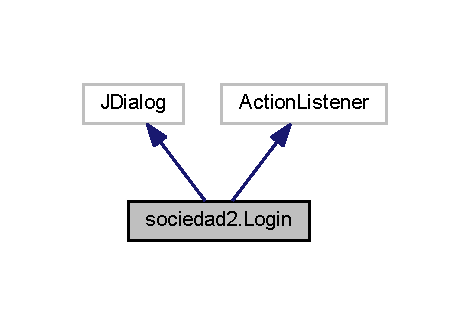
\includegraphics[width=226pt]{classsociedad2_1_1_login__inherit__graph}
\end{center}
\end{figure}


Collaboration diagram for sociedad2.\+Login\+:
\nopagebreak
\begin{figure}[H]
\begin{center}
\leavevmode
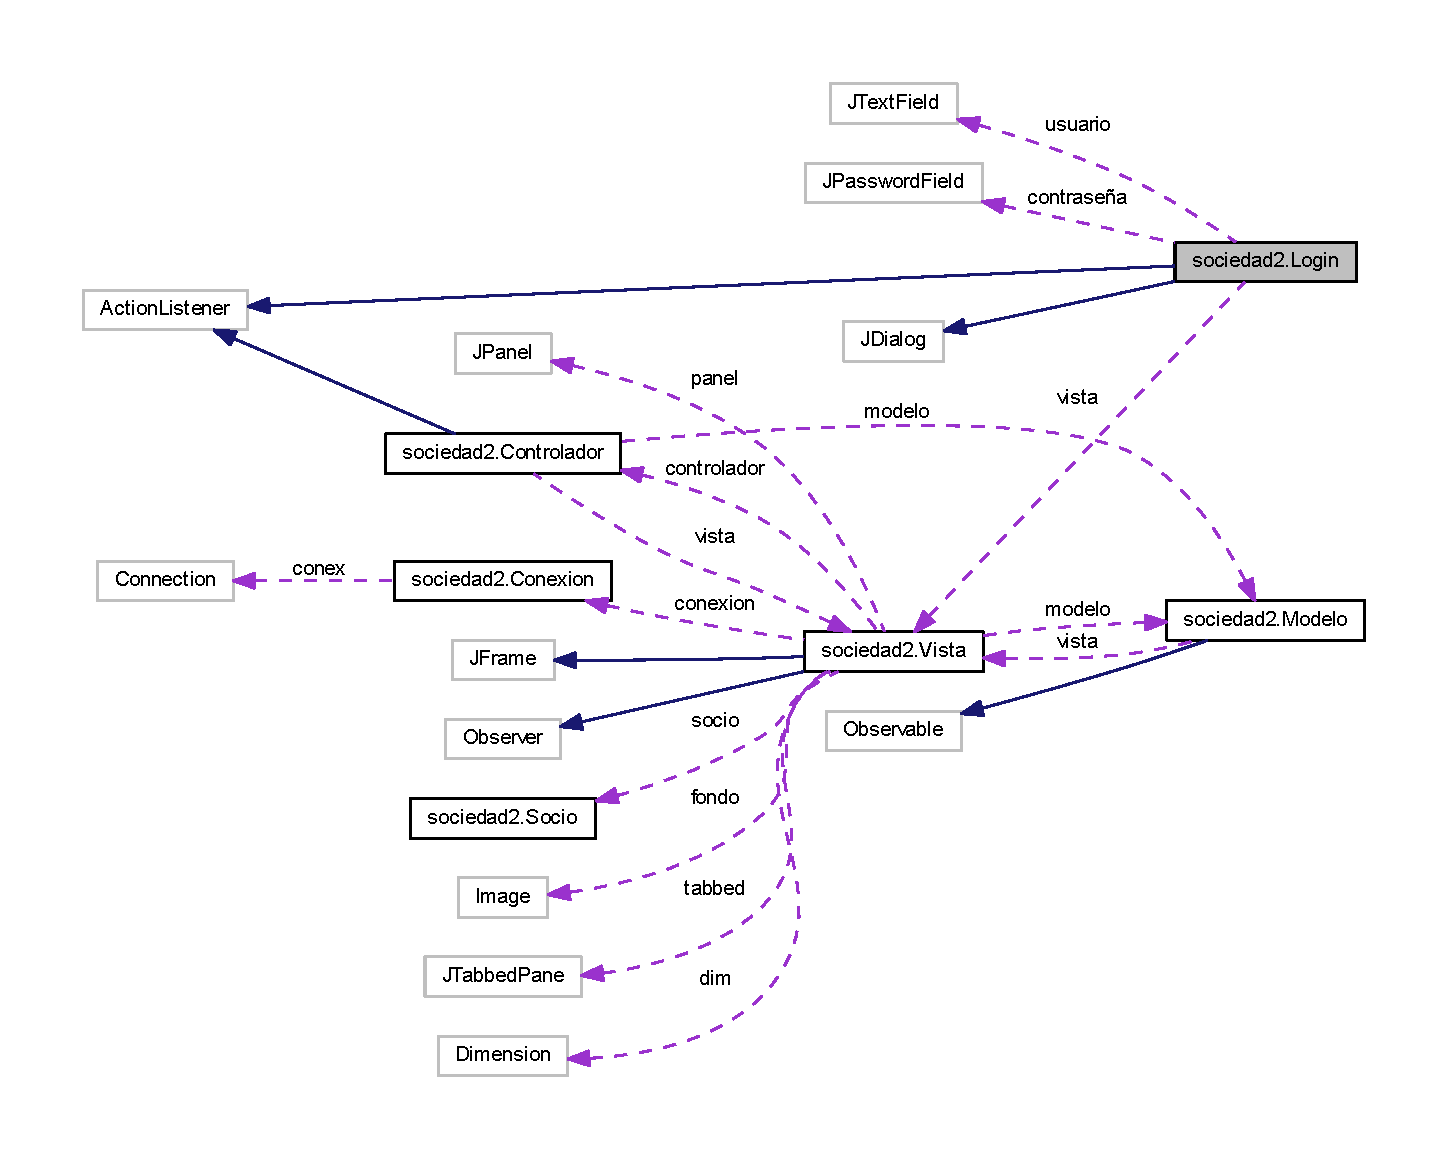
\includegraphics[width=350pt]{classsociedad2_1_1_login__coll__graph}
\end{center}
\end{figure}
\subsection*{Public Member Functions}
\begin{DoxyCompactItemize}
\item 
\mbox{\hyperlink{classsociedad2_1_1_login_a41135064a97e4de4695a8d07074c35d6}{Login}} (\mbox{\hyperlink{classsociedad2_1_1_vista}{Vista}} vista)
\item 
Container \mbox{\hyperlink{classsociedad2_1_1_login_aca75f65b08cee82c43dccbfeb102b7d2}{panel\+Botones}} ()
\item 
Container \mbox{\hyperlink{classsociedad2_1_1_login_a08c7dd2e394966f747492b9bb70a6014}{crear\+Botones}} (String titulo)
\item 
void \mbox{\hyperlink{classsociedad2_1_1_login_ab4f019526871938dfc3f8bdd78c56650}{action\+Performed}} (Action\+Event e)
\end{DoxyCompactItemize}


\subsection{Detailed Description}


Definition at line 20 of file Login.\+java.



\subsection{Constructor \& Destructor Documentation}
\mbox{\Hypertarget{classsociedad2_1_1_login_a41135064a97e4de4695a8d07074c35d6}\label{classsociedad2_1_1_login_a41135064a97e4de4695a8d07074c35d6}} 
\index{sociedad2\+::\+Login@{sociedad2\+::\+Login}!Login@{Login}}
\index{Login@{Login}!sociedad2\+::\+Login@{sociedad2\+::\+Login}}
\subsubsection{\texorpdfstring{Login()}{Login()}}
{\footnotesize\ttfamily sociedad2.\+Login.\+Login (\begin{DoxyParamCaption}\item[{\mbox{\hyperlink{classsociedad2_1_1_vista}{Vista}}}]{vista }\end{DoxyParamCaption})}



Definition at line 25 of file Login.\+java.



\subsection{Member Function Documentation}
\mbox{\Hypertarget{classsociedad2_1_1_login_ab4f019526871938dfc3f8bdd78c56650}\label{classsociedad2_1_1_login_ab4f019526871938dfc3f8bdd78c56650}} 
\index{sociedad2\+::\+Login@{sociedad2\+::\+Login}!action\+Performed@{action\+Performed}}
\index{action\+Performed@{action\+Performed}!sociedad2\+::\+Login@{sociedad2\+::\+Login}}
\subsubsection{\texorpdfstring{action\+Performed()}{actionPerformed()}}
{\footnotesize\ttfamily void sociedad2.\+Login.\+action\+Performed (\begin{DoxyParamCaption}\item[{Action\+Event}]{e }\end{DoxyParamCaption})}



Definition at line 95 of file Login.\+java.

\mbox{\Hypertarget{classsociedad2_1_1_login_a08c7dd2e394966f747492b9bb70a6014}\label{classsociedad2_1_1_login_a08c7dd2e394966f747492b9bb70a6014}} 
\index{sociedad2\+::\+Login@{sociedad2\+::\+Login}!crear\+Botones@{crear\+Botones}}
\index{crear\+Botones@{crear\+Botones}!sociedad2\+::\+Login@{sociedad2\+::\+Login}}
\subsubsection{\texorpdfstring{crear\+Botones()}{crearBotones()}}
{\footnotesize\ttfamily Container sociedad2.\+Login.\+crear\+Botones (\begin{DoxyParamCaption}\item[{String}]{titulo }\end{DoxyParamCaption})}



Definition at line 84 of file Login.\+java.

\mbox{\Hypertarget{classsociedad2_1_1_login_aca75f65b08cee82c43dccbfeb102b7d2}\label{classsociedad2_1_1_login_aca75f65b08cee82c43dccbfeb102b7d2}} 
\index{sociedad2\+::\+Login@{sociedad2\+::\+Login}!panel\+Botones@{panel\+Botones}}
\index{panel\+Botones@{panel\+Botones}!sociedad2\+::\+Login@{sociedad2\+::\+Login}}
\subsubsection{\texorpdfstring{panel\+Botones()}{panelBotones()}}
{\footnotesize\ttfamily Container sociedad2.\+Login.\+panel\+Botones (\begin{DoxyParamCaption}{ }\end{DoxyParamCaption})}



Definition at line 73 of file Login.\+java.



The documentation for this class was generated from the following file\+:\begin{DoxyCompactItemize}
\item 
E\+:/eclipse-\/workspace/\+Sociedad/src/sociedad2/\mbox{\hyperlink{_login_8java}{Login.\+java}}\end{DoxyCompactItemize}

\hypertarget{classsociedad2_1_1_mi_adaptador}{}\section{sociedad2.\+Mi\+Adaptador Class Reference}
\label{classsociedad2_1_1_mi_adaptador}\index{sociedad2.\+Mi\+Adaptador@{sociedad2.\+Mi\+Adaptador}}


Inheritance diagram for sociedad2.\+Mi\+Adaptador\+:
\nopagebreak
\begin{figure}[H]
\begin{center}
\leavevmode
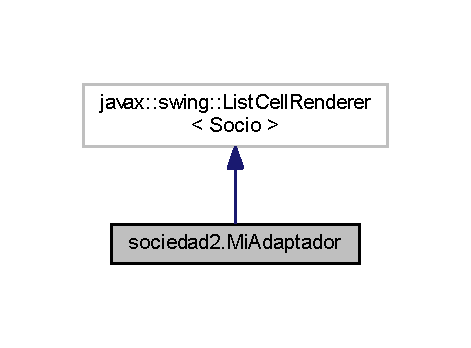
\includegraphics[width=226pt]{classsociedad2_1_1_mi_adaptador__inherit__graph}
\end{center}
\end{figure}


Collaboration diagram for sociedad2.\+Mi\+Adaptador\+:
\nopagebreak
\begin{figure}[H]
\begin{center}
\leavevmode
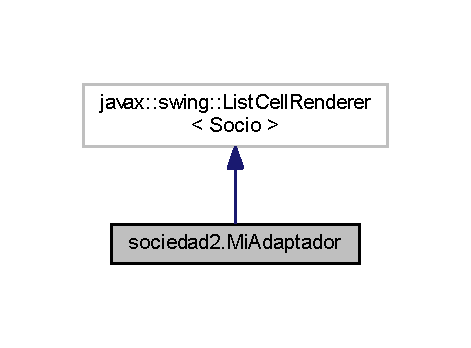
\includegraphics[width=226pt]{classsociedad2_1_1_mi_adaptador__coll__graph}
\end{center}
\end{figure}
\subsection*{Public Member Functions}
\begin{DoxyCompactItemize}
\item 
Component \mbox{\hyperlink{classsociedad2_1_1_mi_adaptador_a27def0784983d566dabf88f07bbdd913}{get\+List\+Cell\+Renderer\+Component}} (J\+List$<$? extends \mbox{\hyperlink{classsociedad2_1_1_socio}{Socio}} $>$ list, \mbox{\hyperlink{classsociedad2_1_1_socio}{Socio}} p, int index, boolean is\+Selected, boolean cell\+Has\+Focus)
\end{DoxyCompactItemize}


\subsection{Detailed Description}


Definition at line 19 of file Mi\+Adaptador.\+java.



\subsection{Member Function Documentation}
\mbox{\Hypertarget{classsociedad2_1_1_mi_adaptador_a27def0784983d566dabf88f07bbdd913}\label{classsociedad2_1_1_mi_adaptador_a27def0784983d566dabf88f07bbdd913}} 
\index{sociedad2\+::\+Mi\+Adaptador@{sociedad2\+::\+Mi\+Adaptador}!get\+List\+Cell\+Renderer\+Component@{get\+List\+Cell\+Renderer\+Component}}
\index{get\+List\+Cell\+Renderer\+Component@{get\+List\+Cell\+Renderer\+Component}!sociedad2\+::\+Mi\+Adaptador@{sociedad2\+::\+Mi\+Adaptador}}
\subsubsection{\texorpdfstring{get\+List\+Cell\+Renderer\+Component()}{getListCellRendererComponent()}}
{\footnotesize\ttfamily Component sociedad2.\+Mi\+Adaptador.\+get\+List\+Cell\+Renderer\+Component (\begin{DoxyParamCaption}\item[{J\+List$<$? extends \mbox{\hyperlink{classsociedad2_1_1_socio}{Socio}} $>$}]{list,  }\item[{\mbox{\hyperlink{classsociedad2_1_1_socio}{Socio}}}]{p,  }\item[{int}]{index,  }\item[{boolean}]{is\+Selected,  }\item[{boolean}]{cell\+Has\+Focus }\end{DoxyParamCaption})}



Definition at line 22 of file Mi\+Adaptador.\+java.



The documentation for this class was generated from the following file\+:\begin{DoxyCompactItemize}
\item 
E\+:/eclipse-\/workspace/\+Sociedad/src/sociedad2/\mbox{\hyperlink{_mi_adaptador_8java}{Mi\+Adaptador.\+java}}\end{DoxyCompactItemize}

\hypertarget{classsociedad2_1_1_mi_adaptador_producto}{}\section{sociedad2.\+Mi\+Adaptador\+Producto Class Reference}
\label{classsociedad2_1_1_mi_adaptador_producto}\index{sociedad2.\+Mi\+Adaptador\+Producto@{sociedad2.\+Mi\+Adaptador\+Producto}}


Inheritance diagram for sociedad2.\+Mi\+Adaptador\+Producto\+:
\nopagebreak
\begin{figure}[H]
\begin{center}
\leavevmode
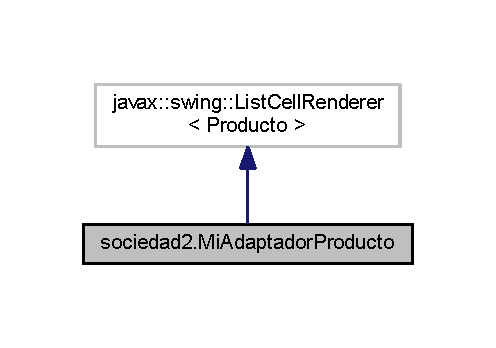
\includegraphics[width=238pt]{classsociedad2_1_1_mi_adaptador_producto__inherit__graph}
\end{center}
\end{figure}


Collaboration diagram for sociedad2.\+Mi\+Adaptador\+Producto\+:
\nopagebreak
\begin{figure}[H]
\begin{center}
\leavevmode
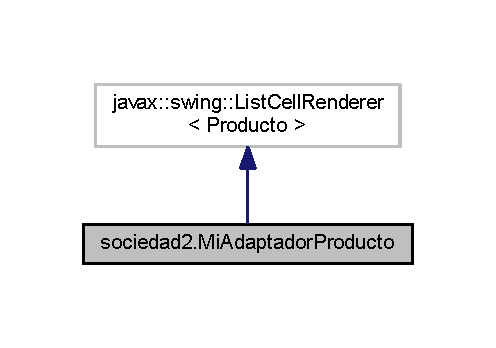
\includegraphics[width=238pt]{classsociedad2_1_1_mi_adaptador_producto__coll__graph}
\end{center}
\end{figure}
\subsection*{Public Member Functions}
\begin{DoxyCompactItemize}
\item 
Component \mbox{\hyperlink{classsociedad2_1_1_mi_adaptador_producto_af202727879511339e4a8916d8e7f3be5}{get\+List\+Cell\+Renderer\+Component}} (J\+List$<$? extends \mbox{\hyperlink{classsociedad2_1_1_producto}{Producto}} $>$ list, \mbox{\hyperlink{classsociedad2_1_1_producto}{Producto}} p, int index, boolean is\+Selected, boolean cell\+Has\+Focus)
\end{DoxyCompactItemize}


\subsection{Detailed Description}


Definition at line 16 of file Mi\+Adaptador\+Producto.\+java.



\subsection{Member Function Documentation}
\mbox{\Hypertarget{classsociedad2_1_1_mi_adaptador_producto_af202727879511339e4a8916d8e7f3be5}\label{classsociedad2_1_1_mi_adaptador_producto_af202727879511339e4a8916d8e7f3be5}} 
\index{sociedad2\+::\+Mi\+Adaptador\+Producto@{sociedad2\+::\+Mi\+Adaptador\+Producto}!get\+List\+Cell\+Renderer\+Component@{get\+List\+Cell\+Renderer\+Component}}
\index{get\+List\+Cell\+Renderer\+Component@{get\+List\+Cell\+Renderer\+Component}!sociedad2\+::\+Mi\+Adaptador\+Producto@{sociedad2\+::\+Mi\+Adaptador\+Producto}}
\subsubsection{\texorpdfstring{get\+List\+Cell\+Renderer\+Component()}{getListCellRendererComponent()}}
{\footnotesize\ttfamily Component sociedad2.\+Mi\+Adaptador\+Producto.\+get\+List\+Cell\+Renderer\+Component (\begin{DoxyParamCaption}\item[{J\+List$<$? extends \mbox{\hyperlink{classsociedad2_1_1_producto}{Producto}} $>$}]{list,  }\item[{\mbox{\hyperlink{classsociedad2_1_1_producto}{Producto}}}]{p,  }\item[{int}]{index,  }\item[{boolean}]{is\+Selected,  }\item[{boolean}]{cell\+Has\+Focus }\end{DoxyParamCaption})}



Definition at line 19 of file Mi\+Adaptador\+Producto.\+java.



The documentation for this class was generated from the following file\+:\begin{DoxyCompactItemize}
\item 
E\+:/eclipse-\/workspace/\+Sociedad/src/sociedad2/\mbox{\hyperlink{_mi_adaptador_producto_8java}{Mi\+Adaptador\+Producto.\+java}}\end{DoxyCompactItemize}

\hypertarget{classsociedad2_1_1_mi_adaptador_registrar_consumicion}{}\section{sociedad2.\+Mi\+Adaptador\+Registrar\+Consumicion Class Reference}
\label{classsociedad2_1_1_mi_adaptador_registrar_consumicion}\index{sociedad2.\+Mi\+Adaptador\+Registrar\+Consumicion@{sociedad2.\+Mi\+Adaptador\+Registrar\+Consumicion}}


Inheritance diagram for sociedad2.\+Mi\+Adaptador\+Registrar\+Consumicion\+:
\nopagebreak
\begin{figure}[H]
\begin{center}
\leavevmode
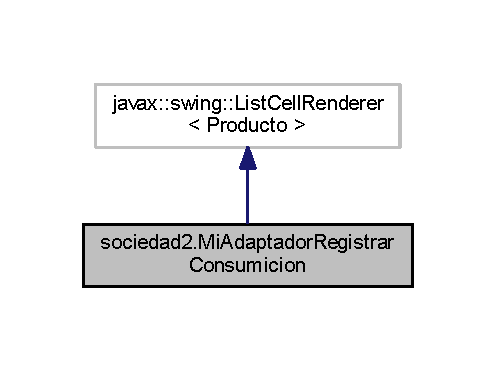
\includegraphics[width=238pt]{classsociedad2_1_1_mi_adaptador_registrar_consumicion__inherit__graph}
\end{center}
\end{figure}


Collaboration diagram for sociedad2.\+Mi\+Adaptador\+Registrar\+Consumicion\+:
\nopagebreak
\begin{figure}[H]
\begin{center}
\leavevmode
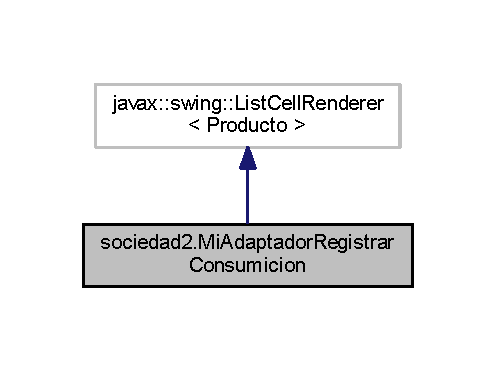
\includegraphics[width=238pt]{classsociedad2_1_1_mi_adaptador_registrar_consumicion__coll__graph}
\end{center}
\end{figure}
\subsection*{Public Member Functions}
\begin{DoxyCompactItemize}
\item 
Component \mbox{\hyperlink{classsociedad2_1_1_mi_adaptador_registrar_consumicion_ad2e140e505196acfa5a6e53a46486387}{get\+List\+Cell\+Renderer\+Component}} (J\+List$<$? extends \mbox{\hyperlink{classsociedad2_1_1_producto}{Producto}} $>$ list, \mbox{\hyperlink{classsociedad2_1_1_producto}{Producto}} p, int index, boolean is\+Selected, boolean cell\+Has\+Focus)
\end{DoxyCompactItemize}


\subsection{Detailed Description}


Definition at line 18 of file Mi\+Adaptador\+Registrar\+Consumicion.\+java.



\subsection{Member Function Documentation}
\mbox{\Hypertarget{classsociedad2_1_1_mi_adaptador_registrar_consumicion_ad2e140e505196acfa5a6e53a46486387}\label{classsociedad2_1_1_mi_adaptador_registrar_consumicion_ad2e140e505196acfa5a6e53a46486387}} 
\index{sociedad2\+::\+Mi\+Adaptador\+Registrar\+Consumicion@{sociedad2\+::\+Mi\+Adaptador\+Registrar\+Consumicion}!get\+List\+Cell\+Renderer\+Component@{get\+List\+Cell\+Renderer\+Component}}
\index{get\+List\+Cell\+Renderer\+Component@{get\+List\+Cell\+Renderer\+Component}!sociedad2\+::\+Mi\+Adaptador\+Registrar\+Consumicion@{sociedad2\+::\+Mi\+Adaptador\+Registrar\+Consumicion}}
\subsubsection{\texorpdfstring{get\+List\+Cell\+Renderer\+Component()}{getListCellRendererComponent()}}
{\footnotesize\ttfamily Component sociedad2.\+Mi\+Adaptador\+Registrar\+Consumicion.\+get\+List\+Cell\+Renderer\+Component (\begin{DoxyParamCaption}\item[{J\+List$<$? extends \mbox{\hyperlink{classsociedad2_1_1_producto}{Producto}} $>$}]{list,  }\item[{\mbox{\hyperlink{classsociedad2_1_1_producto}{Producto}}}]{p,  }\item[{int}]{index,  }\item[{boolean}]{is\+Selected,  }\item[{boolean}]{cell\+Has\+Focus }\end{DoxyParamCaption})}



Definition at line 23 of file Mi\+Adaptador\+Registrar\+Consumicion.\+java.



The documentation for this class was generated from the following file\+:\begin{DoxyCompactItemize}
\item 
E\+:/eclipse-\/workspace/\+Sociedad/src/sociedad2/\mbox{\hyperlink{_mi_adaptador_registrar_consumicion_8java}{Mi\+Adaptador\+Registrar\+Consumicion.\+java}}\end{DoxyCompactItemize}

\hypertarget{classsociedad2_1_1_mi_panel}{}\section{sociedad2.\+Mi\+Panel Class Reference}
\label{classsociedad2_1_1_mi_panel}\index{sociedad2.\+Mi\+Panel@{sociedad2.\+Mi\+Panel}}


Inheritance diagram for sociedad2.\+Mi\+Panel\+:\nopagebreak
\begin{figure}[H]
\begin{center}
\leavevmode
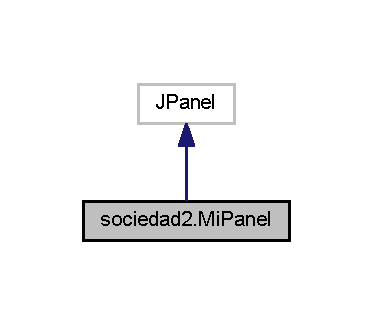
\includegraphics[width=179pt]{classsociedad2_1_1_mi_panel__inherit__graph}
\end{center}
\end{figure}


Collaboration diagram for sociedad2.\+Mi\+Panel\+:\nopagebreak
\begin{figure}[H]
\begin{center}
\leavevmode
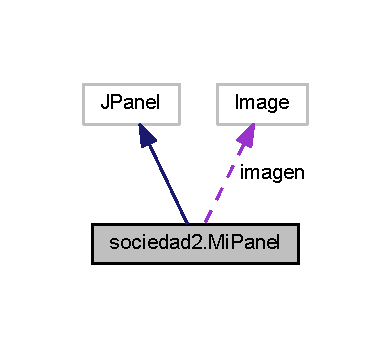
\includegraphics[width=188pt]{classsociedad2_1_1_mi_panel__coll__graph}
\end{center}
\end{figure}
\subsection*{Public Member Functions}
\begin{DoxyCompactItemize}
\item 
\mbox{\hyperlink{classsociedad2_1_1_mi_panel_a728fc4503e18ffec92d5391ef75f7f40}{Mi\+Panel}} (Image imagen)
\item 
void \mbox{\hyperlink{classsociedad2_1_1_mi_panel_a94a0438f3a9cdbb34b254eed58037304}{set\+Imagen}} (Image nueva\+Imagen)
\end{DoxyCompactItemize}
\subsection*{Protected Member Functions}
\begin{DoxyCompactItemize}
\item 
void \mbox{\hyperlink{classsociedad2_1_1_mi_panel_a6dc4cf9761290c785f3d046799043ad4}{paint\+Component}} (Graphics g)
\end{DoxyCompactItemize}


\subsection{Detailed Description}


Definition at line 11 of file Mi\+Panel.\+java.



\subsection{Constructor \& Destructor Documentation}
\mbox{\Hypertarget{classsociedad2_1_1_mi_panel_a728fc4503e18ffec92d5391ef75f7f40}\label{classsociedad2_1_1_mi_panel_a728fc4503e18ffec92d5391ef75f7f40}} 
\index{sociedad2\+::\+Mi\+Panel@{sociedad2\+::\+Mi\+Panel}!Mi\+Panel@{Mi\+Panel}}
\index{Mi\+Panel@{Mi\+Panel}!sociedad2\+::\+Mi\+Panel@{sociedad2\+::\+Mi\+Panel}}
\subsubsection{\texorpdfstring{Mi\+Panel()}{MiPanel()}}
{\footnotesize\ttfamily sociedad2.\+Mi\+Panel.\+Mi\+Panel (\begin{DoxyParamCaption}\item[{Image}]{imagen }\end{DoxyParamCaption})}



Definition at line 15 of file Mi\+Panel.\+java.



\subsection{Member Function Documentation}
\mbox{\Hypertarget{classsociedad2_1_1_mi_panel_a6dc4cf9761290c785f3d046799043ad4}\label{classsociedad2_1_1_mi_panel_a6dc4cf9761290c785f3d046799043ad4}} 
\index{sociedad2\+::\+Mi\+Panel@{sociedad2\+::\+Mi\+Panel}!paint\+Component@{paint\+Component}}
\index{paint\+Component@{paint\+Component}!sociedad2\+::\+Mi\+Panel@{sociedad2\+::\+Mi\+Panel}}
\subsubsection{\texorpdfstring{paint\+Component()}{paintComponent()}}
{\footnotesize\ttfamily void sociedad2.\+Mi\+Panel.\+paint\+Component (\begin{DoxyParamCaption}\item[{Graphics}]{g }\end{DoxyParamCaption})\hspace{0.3cm}{\ttfamily [protected]}}



Definition at line 28 of file Mi\+Panel.\+java.

\mbox{\Hypertarget{classsociedad2_1_1_mi_panel_a94a0438f3a9cdbb34b254eed58037304}\label{classsociedad2_1_1_mi_panel_a94a0438f3a9cdbb34b254eed58037304}} 
\index{sociedad2\+::\+Mi\+Panel@{sociedad2\+::\+Mi\+Panel}!set\+Imagen@{set\+Imagen}}
\index{set\+Imagen@{set\+Imagen}!sociedad2\+::\+Mi\+Panel@{sociedad2\+::\+Mi\+Panel}}
\subsubsection{\texorpdfstring{set\+Imagen()}{setImagen()}}
{\footnotesize\ttfamily void sociedad2.\+Mi\+Panel.\+set\+Imagen (\begin{DoxyParamCaption}\item[{Image}]{nueva\+Imagen }\end{DoxyParamCaption})}



Definition at line 21 of file Mi\+Panel.\+java.



The documentation for this class was generated from the following file\+:\begin{DoxyCompactItemize}
\item 
E\+:/eclipse-\/workspace/\+Sociedad/src/sociedad2/\mbox{\hyperlink{_mi_panel_8java}{Mi\+Panel.\+java}}\end{DoxyCompactItemize}

\hypertarget{classsociedad2_1_1_modelo}{}\section{sociedad2.\+Modelo Class Reference}
\label{classsociedad2_1_1_modelo}\index{sociedad2.\+Modelo@{sociedad2.\+Modelo}}


Inheritance diagram for sociedad2.\+Modelo\+:\nopagebreak
\begin{figure}[H]
\begin{center}
\leavevmode
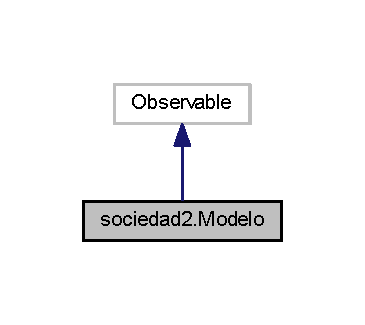
\includegraphics[width=175pt]{classsociedad2_1_1_modelo__inherit__graph}
\end{center}
\end{figure}


Collaboration diagram for sociedad2.\+Modelo\+:
\nopagebreak
\begin{figure}[H]
\begin{center}
\leavevmode
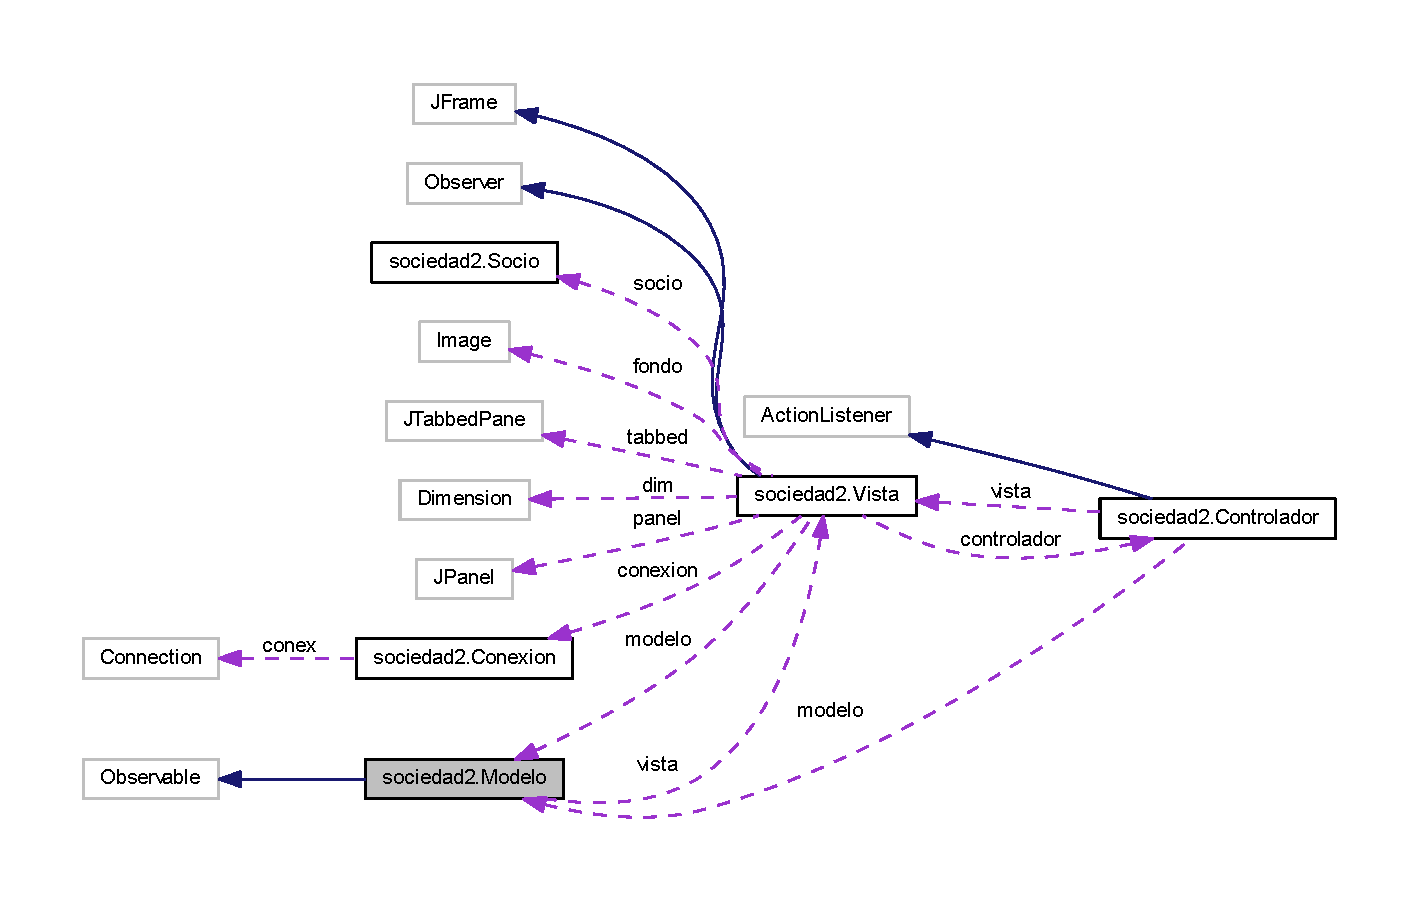
\includegraphics[width=350pt]{classsociedad2_1_1_modelo__coll__graph}
\end{center}
\end{figure}
\subsection*{Public Member Functions}
\begin{DoxyCompactItemize}
\item 
\mbox{\hyperlink{classsociedad2_1_1_modelo_a86845e60b689ec38e858bde11723e6ef}{Modelo}} (\mbox{\hyperlink{classsociedad2_1_1_vista}{Vista}} vista)
\item 
Array\+List$<$ \mbox{\hyperlink{classsociedad2_1_1_socio}{Socio}} $>$ \mbox{\hyperlink{classsociedad2_1_1_modelo_a6d7ac9cc5eeccf4a421552249ffd81a3}{Consultar\+Datos\+Socio}} (String comando, String info, Connection con)  throws S\+Q\+L\+Exception 
\item 
Array\+List$<$ \mbox{\hyperlink{classsociedad2_1_1_producto}{Producto}} $>$ \mbox{\hyperlink{classsociedad2_1_1_modelo_acee3bbd6bb68da5cdecf4f91b442c420}{Consultar\+Datos\+Productos}} (String comando, String info, Connection con)  throws S\+Q\+L\+Exception 
\item 
Array\+List$<$ \mbox{\hyperlink{classsociedad2_1_1_categorias}{Categorias}} $>$ \mbox{\hyperlink{classsociedad2_1_1_modelo_ad5d24bd98199dc5f80dc16de9dcb7287}{Consultar\+Datos\+Categorias}} (String comando, String info, Connection con)  throws S\+Q\+L\+Exception 
\item 
void \mbox{\hyperlink{classsociedad2_1_1_modelo_a19514d1ec71bfec488ee6712ee43c9cc}{insertar\+Datos}} (String comando, Connection conn)
\item 
int \mbox{\hyperlink{classsociedad2_1_1_modelo_acbf5f90be2a155ebac005a274b812fe7}{obtener\+Id}} (String comando, Connection conn)
\item 
void \mbox{\hyperlink{classsociedad2_1_1_modelo_a650c4ed5505b43ee33c1064d8413c645}{comprobar}} ()
\item 
void \mbox{\hyperlink{classsociedad2_1_1_modelo_a90980190a9a1aa4bec012b891335e3a0}{sacar\+Alerta\+Productos\+Minimo}} (Array\+List$<$ \mbox{\hyperlink{classsociedad2_1_1_producto}{Producto}} $>$ lista)
\item 
void \mbox{\hyperlink{classsociedad2_1_1_modelo_a8b79e5db8e4ec13de96078a91f7d2741}{hacer\+Pedido}} (Array\+List$<$ \mbox{\hyperlink{classsociedad2_1_1_producto}{Producto}} $>$ lista)
\item 
void \mbox{\hyperlink{classsociedad2_1_1_modelo_a66758d80d56ab3bb2f7b031063808eb5}{a�adir\+Pedido}} (Array\+List$<$ \mbox{\hyperlink{classsociedad2_1_1_producto}{Producto}} $>$ lista)
\item 
boolean \mbox{\hyperlink{classsociedad2_1_1_modelo_af10264132f4de68b5ce88891146cd27e}{identificarse}} (String s1, String s2, Connection con)
\end{DoxyCompactItemize}


\subsection{Detailed Description}


Definition at line 26 of file Modelo.\+java.



\subsection{Constructor \& Destructor Documentation}
\mbox{\Hypertarget{classsociedad2_1_1_modelo_a86845e60b689ec38e858bde11723e6ef}\label{classsociedad2_1_1_modelo_a86845e60b689ec38e858bde11723e6ef}} 
\index{sociedad2\+::\+Modelo@{sociedad2\+::\+Modelo}!Modelo@{Modelo}}
\index{Modelo@{Modelo}!sociedad2\+::\+Modelo@{sociedad2\+::\+Modelo}}
\subsubsection{\texorpdfstring{Modelo()}{Modelo()}}
{\footnotesize\ttfamily sociedad2.\+Modelo.\+Modelo (\begin{DoxyParamCaption}\item[{\mbox{\hyperlink{classsociedad2_1_1_vista}{Vista}}}]{vista }\end{DoxyParamCaption})}



Definition at line 31 of file Modelo.\+java.



\subsection{Member Function Documentation}
\mbox{\Hypertarget{classsociedad2_1_1_modelo_a66758d80d56ab3bb2f7b031063808eb5}\label{classsociedad2_1_1_modelo_a66758d80d56ab3bb2f7b031063808eb5}} 
\index{sociedad2\+::\+Modelo@{sociedad2\+::\+Modelo}!a�adir\+Pedido@{a�adir\+Pedido}}
\index{a�adir\+Pedido@{a�adir\+Pedido}!sociedad2\+::\+Modelo@{sociedad2\+::\+Modelo}}
\subsubsection{\texorpdfstring{a�adir\+Pedido()}{a�adirPedido()}}
{\footnotesize\ttfamily void sociedad2.\+Modelo.\+a�adir\+Pedido (\begin{DoxyParamCaption}\item[{Array\+List$<$ \mbox{\hyperlink{classsociedad2_1_1_producto}{Producto}} $>$}]{lista }\end{DoxyParamCaption})}



Definition at line 254 of file Modelo.\+java.

\mbox{\Hypertarget{classsociedad2_1_1_modelo_a650c4ed5505b43ee33c1064d8413c645}\label{classsociedad2_1_1_modelo_a650c4ed5505b43ee33c1064d8413c645}} 
\index{sociedad2\+::\+Modelo@{sociedad2\+::\+Modelo}!comprobar@{comprobar}}
\index{comprobar@{comprobar}!sociedad2\+::\+Modelo@{sociedad2\+::\+Modelo}}
\subsubsection{\texorpdfstring{comprobar()}{comprobar()}}
{\footnotesize\ttfamily void sociedad2.\+Modelo.\+comprobar (\begin{DoxyParamCaption}{ }\end{DoxyParamCaption})}



Definition at line 137 of file Modelo.\+java.

\mbox{\Hypertarget{classsociedad2_1_1_modelo_ad5d24bd98199dc5f80dc16de9dcb7287}\label{classsociedad2_1_1_modelo_ad5d24bd98199dc5f80dc16de9dcb7287}} 
\index{sociedad2\+::\+Modelo@{sociedad2\+::\+Modelo}!Consultar\+Datos\+Categorias@{Consultar\+Datos\+Categorias}}
\index{Consultar\+Datos\+Categorias@{Consultar\+Datos\+Categorias}!sociedad2\+::\+Modelo@{sociedad2\+::\+Modelo}}
\subsubsection{\texorpdfstring{Consultar\+Datos\+Categorias()}{ConsultarDatosCategorias()}}
{\footnotesize\ttfamily Array\+List$<$\mbox{\hyperlink{classsociedad2_1_1_categorias}{Categorias}}$>$ sociedad2.\+Modelo.\+Consultar\+Datos\+Categorias (\begin{DoxyParamCaption}\item[{String}]{comando,  }\item[{String}]{info,  }\item[{Connection}]{con }\end{DoxyParamCaption}) throws S\+Q\+L\+Exception}



Definition at line 75 of file Modelo.\+java.

\mbox{\Hypertarget{classsociedad2_1_1_modelo_acee3bbd6bb68da5cdecf4f91b442c420}\label{classsociedad2_1_1_modelo_acee3bbd6bb68da5cdecf4f91b442c420}} 
\index{sociedad2\+::\+Modelo@{sociedad2\+::\+Modelo}!Consultar\+Datos\+Productos@{Consultar\+Datos\+Productos}}
\index{Consultar\+Datos\+Productos@{Consultar\+Datos\+Productos}!sociedad2\+::\+Modelo@{sociedad2\+::\+Modelo}}
\subsubsection{\texorpdfstring{Consultar\+Datos\+Productos()}{ConsultarDatosProductos()}}
{\footnotesize\ttfamily Array\+List$<$\mbox{\hyperlink{classsociedad2_1_1_producto}{Producto}}$>$ sociedad2.\+Modelo.\+Consultar\+Datos\+Productos (\begin{DoxyParamCaption}\item[{String}]{comando,  }\item[{String}]{info,  }\item[{Connection}]{con }\end{DoxyParamCaption}) throws S\+Q\+L\+Exception}



Definition at line 56 of file Modelo.\+java.

\mbox{\Hypertarget{classsociedad2_1_1_modelo_a6d7ac9cc5eeccf4a421552249ffd81a3}\label{classsociedad2_1_1_modelo_a6d7ac9cc5eeccf4a421552249ffd81a3}} 
\index{sociedad2\+::\+Modelo@{sociedad2\+::\+Modelo}!Consultar\+Datos\+Socio@{Consultar\+Datos\+Socio}}
\index{Consultar\+Datos\+Socio@{Consultar\+Datos\+Socio}!sociedad2\+::\+Modelo@{sociedad2\+::\+Modelo}}
\subsubsection{\texorpdfstring{Consultar\+Datos\+Socio()}{ConsultarDatosSocio()}}
{\footnotesize\ttfamily Array\+List$<$\mbox{\hyperlink{classsociedad2_1_1_socio}{Socio}}$>$ sociedad2.\+Modelo.\+Consultar\+Datos\+Socio (\begin{DoxyParamCaption}\item[{String}]{comando,  }\item[{String}]{info,  }\item[{Connection}]{con }\end{DoxyParamCaption}) throws S\+Q\+L\+Exception}



Definition at line 37 of file Modelo.\+java.

\mbox{\Hypertarget{classsociedad2_1_1_modelo_a8b79e5db8e4ec13de96078a91f7d2741}\label{classsociedad2_1_1_modelo_a8b79e5db8e4ec13de96078a91f7d2741}} 
\index{sociedad2\+::\+Modelo@{sociedad2\+::\+Modelo}!hacer\+Pedido@{hacer\+Pedido}}
\index{hacer\+Pedido@{hacer\+Pedido}!sociedad2\+::\+Modelo@{sociedad2\+::\+Modelo}}
\subsubsection{\texorpdfstring{hacer\+Pedido()}{hacerPedido()}}
{\footnotesize\ttfamily void sociedad2.\+Modelo.\+hacer\+Pedido (\begin{DoxyParamCaption}\item[{Array\+List$<$ \mbox{\hyperlink{classsociedad2_1_1_producto}{Producto}} $>$}]{lista }\end{DoxyParamCaption})}



Definition at line 185 of file Modelo.\+java.

\mbox{\Hypertarget{classsociedad2_1_1_modelo_af10264132f4de68b5ce88891146cd27e}\label{classsociedad2_1_1_modelo_af10264132f4de68b5ce88891146cd27e}} 
\index{sociedad2\+::\+Modelo@{sociedad2\+::\+Modelo}!identificarse@{identificarse}}
\index{identificarse@{identificarse}!sociedad2\+::\+Modelo@{sociedad2\+::\+Modelo}}
\subsubsection{\texorpdfstring{identificarse()}{identificarse()}}
{\footnotesize\ttfamily boolean sociedad2.\+Modelo.\+identificarse (\begin{DoxyParamCaption}\item[{String}]{s1,  }\item[{String}]{s2,  }\item[{Connection}]{con }\end{DoxyParamCaption})}



Definition at line 287 of file Modelo.\+java.

\mbox{\Hypertarget{classsociedad2_1_1_modelo_a19514d1ec71bfec488ee6712ee43c9cc}\label{classsociedad2_1_1_modelo_a19514d1ec71bfec488ee6712ee43c9cc}} 
\index{sociedad2\+::\+Modelo@{sociedad2\+::\+Modelo}!insertar\+Datos@{insertar\+Datos}}
\index{insertar\+Datos@{insertar\+Datos}!sociedad2\+::\+Modelo@{sociedad2\+::\+Modelo}}
\subsubsection{\texorpdfstring{insertar\+Datos()}{insertarDatos()}}
{\footnotesize\ttfamily void sociedad2.\+Modelo.\+insertar\+Datos (\begin{DoxyParamCaption}\item[{String}]{comando,  }\item[{Connection}]{conn }\end{DoxyParamCaption})}



Definition at line 92 of file Modelo.\+java.

\mbox{\Hypertarget{classsociedad2_1_1_modelo_acbf5f90be2a155ebac005a274b812fe7}\label{classsociedad2_1_1_modelo_acbf5f90be2a155ebac005a274b812fe7}} 
\index{sociedad2\+::\+Modelo@{sociedad2\+::\+Modelo}!obtener\+Id@{obtener\+Id}}
\index{obtener\+Id@{obtener\+Id}!sociedad2\+::\+Modelo@{sociedad2\+::\+Modelo}}
\subsubsection{\texorpdfstring{obtener\+Id()}{obtenerId()}}
{\footnotesize\ttfamily int sociedad2.\+Modelo.\+obtener\+Id (\begin{DoxyParamCaption}\item[{String}]{comando,  }\item[{Connection}]{conn }\end{DoxyParamCaption})}



Definition at line 108 of file Modelo.\+java.

\mbox{\Hypertarget{classsociedad2_1_1_modelo_a90980190a9a1aa4bec012b891335e3a0}\label{classsociedad2_1_1_modelo_a90980190a9a1aa4bec012b891335e3a0}} 
\index{sociedad2\+::\+Modelo@{sociedad2\+::\+Modelo}!sacar\+Alerta\+Productos\+Minimo@{sacar\+Alerta\+Productos\+Minimo}}
\index{sacar\+Alerta\+Productos\+Minimo@{sacar\+Alerta\+Productos\+Minimo}!sociedad2\+::\+Modelo@{sociedad2\+::\+Modelo}}
\subsubsection{\texorpdfstring{sacar\+Alerta\+Productos\+Minimo()}{sacarAlertaProductosMinimo()}}
{\footnotesize\ttfamily void sociedad2.\+Modelo.\+sacar\+Alerta\+Productos\+Minimo (\begin{DoxyParamCaption}\item[{Array\+List$<$ \mbox{\hyperlink{classsociedad2_1_1_producto}{Producto}} $>$}]{lista }\end{DoxyParamCaption})}



Definition at line 167 of file Modelo.\+java.



The documentation for this class was generated from the following file\+:\begin{DoxyCompactItemize}
\item 
E\+:/eclipse-\/workspace/\+Sociedad/src/sociedad2/\mbox{\hyperlink{_modelo_8java}{Modelo.\+java}}\end{DoxyCompactItemize}

\hypertarget{classsociedad2_1_1_producto}{}\section{sociedad2.\+Producto Class Reference}
\label{classsociedad2_1_1_producto}\index{sociedad2.\+Producto@{sociedad2.\+Producto}}
\subsection*{Public Member Functions}
\begin{DoxyCompactItemize}
\item 
\mbox{\hyperlink{classsociedad2_1_1_producto_a5266f0ab65459040df5d351c60f46493}{Producto}} (int producto\+Id, int categoria\+Id, String descripcion, int stock, int min\+Stock, int medio\+Stock, Boolean estado, float precio)
\item 
void \mbox{\hyperlink{classsociedad2_1_1_producto_a6eec5e912ac94e10b15bc0a1e62d3a97}{set\+Cantidad}} (int i)
\item 
int \mbox{\hyperlink{classsociedad2_1_1_producto_ad1dffeff2d5eaa28cb0f4c3120bbf047}{get\+Cantidad}} ()
\item 
Boolean \mbox{\hyperlink{classsociedad2_1_1_producto_a60e7b61c9e1d4d0d1f57edee7871cadf}{get\+Estado}} ()
\item 
void \mbox{\hyperlink{classsociedad2_1_1_producto_a7f286e1bd9c4e7a16ba71cda04477139}{set\+Estado}} (Boolean estado)
\item 
int \mbox{\hyperlink{classsociedad2_1_1_producto_a501aad8759cd86d3bf35387f6f697970}{get\+Producto\+Id}} ()
\item 
void \mbox{\hyperlink{classsociedad2_1_1_producto_a5e27c5c7790d1918a32e71f51f9834f7}{set\+Producto\+Id}} (int producto\+Id)
\item 
int \mbox{\hyperlink{classsociedad2_1_1_producto_af32a011e6aa2e99af8882774a23bd368}{get\+Categoria\+Id}} ()
\item 
void \mbox{\hyperlink{classsociedad2_1_1_producto_a7b59257499e49df811a7e00bcfe3768a}{set\+Categoria\+Id}} (int categoria\+Id)
\item 
String \mbox{\hyperlink{classsociedad2_1_1_producto_a83b7e522c9dc622e0ca99a3b6243b57b}{get\+Descripcion}} ()
\item 
void \mbox{\hyperlink{classsociedad2_1_1_producto_a97c84a0e5bafd15bdc48f868d088fde7}{set\+Descripcion}} (String descripcion)
\item 
int \mbox{\hyperlink{classsociedad2_1_1_producto_ac1efc9575ff90b9af915066d43dd4bd4}{get\+Stock}} ()
\item 
void \mbox{\hyperlink{classsociedad2_1_1_producto_ae8833d16f4253ed066e0d9fb78cfb954}{set\+Stock}} (int stock)
\item 
int \mbox{\hyperlink{classsociedad2_1_1_producto_a16f2c1f7840ee35473804385138ddeb8}{get\+Min\+Stock}} ()
\item 
void \mbox{\hyperlink{classsociedad2_1_1_producto_a65c75efc7095fce58822d557b3c5905e}{set\+Min\+Stock}} (int min\+Stock)
\item 
int \mbox{\hyperlink{classsociedad2_1_1_producto_ac31e436e0f5d5da61bf04ba4991cb6d3}{get\+Medio\+Stock}} ()
\item 
void \mbox{\hyperlink{classsociedad2_1_1_producto_ab9a1a3cd64dbd56b3a7fac66a78b8bd8}{set\+Medio\+Stock}} (int medio\+Stock)
\item 
float \mbox{\hyperlink{classsociedad2_1_1_producto_adac1bb4366dc52eef74b5fba4e7018a7}{get\+Precio}} ()
\item 
void \mbox{\hyperlink{classsociedad2_1_1_producto_afd60e3881905bdd4c196d21c5545eadc}{set\+Precio}} (float precio)
\item 
String \mbox{\hyperlink{classsociedad2_1_1_producto_ae19a8691f8a521ff9eb183083f9ff6f4}{to\+String}} ()
\end{DoxyCompactItemize}


\subsection{Detailed Description}


Definition at line 3 of file Producto.\+java.



\subsection{Constructor \& Destructor Documentation}
\mbox{\Hypertarget{classsociedad2_1_1_producto_a5266f0ab65459040df5d351c60f46493}\label{classsociedad2_1_1_producto_a5266f0ab65459040df5d351c60f46493}} 
\index{sociedad2\+::\+Producto@{sociedad2\+::\+Producto}!Producto@{Producto}}
\index{Producto@{Producto}!sociedad2\+::\+Producto@{sociedad2\+::\+Producto}}
\subsubsection{\texorpdfstring{Producto()}{Producto()}}
{\footnotesize\ttfamily sociedad2.\+Producto.\+Producto (\begin{DoxyParamCaption}\item[{int}]{producto\+Id,  }\item[{int}]{categoria\+Id,  }\item[{String}]{descripcion,  }\item[{int}]{stock,  }\item[{int}]{min\+Stock,  }\item[{int}]{medio\+Stock,  }\item[{Boolean}]{estado,  }\item[{float}]{precio }\end{DoxyParamCaption})}



Definition at line 15 of file Producto.\+java.



\subsection{Member Function Documentation}
\mbox{\Hypertarget{classsociedad2_1_1_producto_ad1dffeff2d5eaa28cb0f4c3120bbf047}\label{classsociedad2_1_1_producto_ad1dffeff2d5eaa28cb0f4c3120bbf047}} 
\index{sociedad2\+::\+Producto@{sociedad2\+::\+Producto}!get\+Cantidad@{get\+Cantidad}}
\index{get\+Cantidad@{get\+Cantidad}!sociedad2\+::\+Producto@{sociedad2\+::\+Producto}}
\subsubsection{\texorpdfstring{get\+Cantidad()}{getCantidad()}}
{\footnotesize\ttfamily int sociedad2.\+Producto.\+get\+Cantidad (\begin{DoxyParamCaption}{ }\end{DoxyParamCaption})}



Definition at line 33 of file Producto.\+java.

\mbox{\Hypertarget{classsociedad2_1_1_producto_af32a011e6aa2e99af8882774a23bd368}\label{classsociedad2_1_1_producto_af32a011e6aa2e99af8882774a23bd368}} 
\index{sociedad2\+::\+Producto@{sociedad2\+::\+Producto}!get\+Categoria\+Id@{get\+Categoria\+Id}}
\index{get\+Categoria\+Id@{get\+Categoria\+Id}!sociedad2\+::\+Producto@{sociedad2\+::\+Producto}}
\subsubsection{\texorpdfstring{get\+Categoria\+Id()}{getCategoriaId()}}
{\footnotesize\ttfamily int sociedad2.\+Producto.\+get\+Categoria\+Id (\begin{DoxyParamCaption}{ }\end{DoxyParamCaption})}



Definition at line 54 of file Producto.\+java.

\mbox{\Hypertarget{classsociedad2_1_1_producto_a83b7e522c9dc622e0ca99a3b6243b57b}\label{classsociedad2_1_1_producto_a83b7e522c9dc622e0ca99a3b6243b57b}} 
\index{sociedad2\+::\+Producto@{sociedad2\+::\+Producto}!get\+Descripcion@{get\+Descripcion}}
\index{get\+Descripcion@{get\+Descripcion}!sociedad2\+::\+Producto@{sociedad2\+::\+Producto}}
\subsubsection{\texorpdfstring{get\+Descripcion()}{getDescripcion()}}
{\footnotesize\ttfamily String sociedad2.\+Producto.\+get\+Descripcion (\begin{DoxyParamCaption}{ }\end{DoxyParamCaption})}



Definition at line 62 of file Producto.\+java.

\mbox{\Hypertarget{classsociedad2_1_1_producto_a60e7b61c9e1d4d0d1f57edee7871cadf}\label{classsociedad2_1_1_producto_a60e7b61c9e1d4d0d1f57edee7871cadf}} 
\index{sociedad2\+::\+Producto@{sociedad2\+::\+Producto}!get\+Estado@{get\+Estado}}
\index{get\+Estado@{get\+Estado}!sociedad2\+::\+Producto@{sociedad2\+::\+Producto}}
\subsubsection{\texorpdfstring{get\+Estado()}{getEstado()}}
{\footnotesize\ttfamily Boolean sociedad2.\+Producto.\+get\+Estado (\begin{DoxyParamCaption}{ }\end{DoxyParamCaption})}



Definition at line 38 of file Producto.\+java.

\mbox{\Hypertarget{classsociedad2_1_1_producto_ac31e436e0f5d5da61bf04ba4991cb6d3}\label{classsociedad2_1_1_producto_ac31e436e0f5d5da61bf04ba4991cb6d3}} 
\index{sociedad2\+::\+Producto@{sociedad2\+::\+Producto}!get\+Medio\+Stock@{get\+Medio\+Stock}}
\index{get\+Medio\+Stock@{get\+Medio\+Stock}!sociedad2\+::\+Producto@{sociedad2\+::\+Producto}}
\subsubsection{\texorpdfstring{get\+Medio\+Stock()}{getMedioStock()}}
{\footnotesize\ttfamily int sociedad2.\+Producto.\+get\+Medio\+Stock (\begin{DoxyParamCaption}{ }\end{DoxyParamCaption})}



Definition at line 86 of file Producto.\+java.

\mbox{\Hypertarget{classsociedad2_1_1_producto_a16f2c1f7840ee35473804385138ddeb8}\label{classsociedad2_1_1_producto_a16f2c1f7840ee35473804385138ddeb8}} 
\index{sociedad2\+::\+Producto@{sociedad2\+::\+Producto}!get\+Min\+Stock@{get\+Min\+Stock}}
\index{get\+Min\+Stock@{get\+Min\+Stock}!sociedad2\+::\+Producto@{sociedad2\+::\+Producto}}
\subsubsection{\texorpdfstring{get\+Min\+Stock()}{getMinStock()}}
{\footnotesize\ttfamily int sociedad2.\+Producto.\+get\+Min\+Stock (\begin{DoxyParamCaption}{ }\end{DoxyParamCaption})}



Definition at line 78 of file Producto.\+java.

\mbox{\Hypertarget{classsociedad2_1_1_producto_adac1bb4366dc52eef74b5fba4e7018a7}\label{classsociedad2_1_1_producto_adac1bb4366dc52eef74b5fba4e7018a7}} 
\index{sociedad2\+::\+Producto@{sociedad2\+::\+Producto}!get\+Precio@{get\+Precio}}
\index{get\+Precio@{get\+Precio}!sociedad2\+::\+Producto@{sociedad2\+::\+Producto}}
\subsubsection{\texorpdfstring{get\+Precio()}{getPrecio()}}
{\footnotesize\ttfamily float sociedad2.\+Producto.\+get\+Precio (\begin{DoxyParamCaption}{ }\end{DoxyParamCaption})}



Definition at line 94 of file Producto.\+java.

\mbox{\Hypertarget{classsociedad2_1_1_producto_a501aad8759cd86d3bf35387f6f697970}\label{classsociedad2_1_1_producto_a501aad8759cd86d3bf35387f6f697970}} 
\index{sociedad2\+::\+Producto@{sociedad2\+::\+Producto}!get\+Producto\+Id@{get\+Producto\+Id}}
\index{get\+Producto\+Id@{get\+Producto\+Id}!sociedad2\+::\+Producto@{sociedad2\+::\+Producto}}
\subsubsection{\texorpdfstring{get\+Producto\+Id()}{getProductoId()}}
{\footnotesize\ttfamily int sociedad2.\+Producto.\+get\+Producto\+Id (\begin{DoxyParamCaption}{ }\end{DoxyParamCaption})}



Definition at line 46 of file Producto.\+java.

\mbox{\Hypertarget{classsociedad2_1_1_producto_ac1efc9575ff90b9af915066d43dd4bd4}\label{classsociedad2_1_1_producto_ac1efc9575ff90b9af915066d43dd4bd4}} 
\index{sociedad2\+::\+Producto@{sociedad2\+::\+Producto}!get\+Stock@{get\+Stock}}
\index{get\+Stock@{get\+Stock}!sociedad2\+::\+Producto@{sociedad2\+::\+Producto}}
\subsubsection{\texorpdfstring{get\+Stock()}{getStock()}}
{\footnotesize\ttfamily int sociedad2.\+Producto.\+get\+Stock (\begin{DoxyParamCaption}{ }\end{DoxyParamCaption})}



Definition at line 70 of file Producto.\+java.

\mbox{\Hypertarget{classsociedad2_1_1_producto_a6eec5e912ac94e10b15bc0a1e62d3a97}\label{classsociedad2_1_1_producto_a6eec5e912ac94e10b15bc0a1e62d3a97}} 
\index{sociedad2\+::\+Producto@{sociedad2\+::\+Producto}!set\+Cantidad@{set\+Cantidad}}
\index{set\+Cantidad@{set\+Cantidad}!sociedad2\+::\+Producto@{sociedad2\+::\+Producto}}
\subsubsection{\texorpdfstring{set\+Cantidad()}{setCantidad()}}
{\footnotesize\ttfamily void sociedad2.\+Producto.\+set\+Cantidad (\begin{DoxyParamCaption}\item[{int}]{i }\end{DoxyParamCaption})}



Definition at line 29 of file Producto.\+java.

\mbox{\Hypertarget{classsociedad2_1_1_producto_a7b59257499e49df811a7e00bcfe3768a}\label{classsociedad2_1_1_producto_a7b59257499e49df811a7e00bcfe3768a}} 
\index{sociedad2\+::\+Producto@{sociedad2\+::\+Producto}!set\+Categoria\+Id@{set\+Categoria\+Id}}
\index{set\+Categoria\+Id@{set\+Categoria\+Id}!sociedad2\+::\+Producto@{sociedad2\+::\+Producto}}
\subsubsection{\texorpdfstring{set\+Categoria\+Id()}{setCategoriaId()}}
{\footnotesize\ttfamily void sociedad2.\+Producto.\+set\+Categoria\+Id (\begin{DoxyParamCaption}\item[{int}]{categoria\+Id }\end{DoxyParamCaption})}



Definition at line 58 of file Producto.\+java.

\mbox{\Hypertarget{classsociedad2_1_1_producto_a97c84a0e5bafd15bdc48f868d088fde7}\label{classsociedad2_1_1_producto_a97c84a0e5bafd15bdc48f868d088fde7}} 
\index{sociedad2\+::\+Producto@{sociedad2\+::\+Producto}!set\+Descripcion@{set\+Descripcion}}
\index{set\+Descripcion@{set\+Descripcion}!sociedad2\+::\+Producto@{sociedad2\+::\+Producto}}
\subsubsection{\texorpdfstring{set\+Descripcion()}{setDescripcion()}}
{\footnotesize\ttfamily void sociedad2.\+Producto.\+set\+Descripcion (\begin{DoxyParamCaption}\item[{String}]{descripcion }\end{DoxyParamCaption})}



Definition at line 66 of file Producto.\+java.

\mbox{\Hypertarget{classsociedad2_1_1_producto_a7f286e1bd9c4e7a16ba71cda04477139}\label{classsociedad2_1_1_producto_a7f286e1bd9c4e7a16ba71cda04477139}} 
\index{sociedad2\+::\+Producto@{sociedad2\+::\+Producto}!set\+Estado@{set\+Estado}}
\index{set\+Estado@{set\+Estado}!sociedad2\+::\+Producto@{sociedad2\+::\+Producto}}
\subsubsection{\texorpdfstring{set\+Estado()}{setEstado()}}
{\footnotesize\ttfamily void sociedad2.\+Producto.\+set\+Estado (\begin{DoxyParamCaption}\item[{Boolean}]{estado }\end{DoxyParamCaption})}



Definition at line 42 of file Producto.\+java.

\mbox{\Hypertarget{classsociedad2_1_1_producto_ab9a1a3cd64dbd56b3a7fac66a78b8bd8}\label{classsociedad2_1_1_producto_ab9a1a3cd64dbd56b3a7fac66a78b8bd8}} 
\index{sociedad2\+::\+Producto@{sociedad2\+::\+Producto}!set\+Medio\+Stock@{set\+Medio\+Stock}}
\index{set\+Medio\+Stock@{set\+Medio\+Stock}!sociedad2\+::\+Producto@{sociedad2\+::\+Producto}}
\subsubsection{\texorpdfstring{set\+Medio\+Stock()}{setMedioStock()}}
{\footnotesize\ttfamily void sociedad2.\+Producto.\+set\+Medio\+Stock (\begin{DoxyParamCaption}\item[{int}]{medio\+Stock }\end{DoxyParamCaption})}



Definition at line 90 of file Producto.\+java.

\mbox{\Hypertarget{classsociedad2_1_1_producto_a65c75efc7095fce58822d557b3c5905e}\label{classsociedad2_1_1_producto_a65c75efc7095fce58822d557b3c5905e}} 
\index{sociedad2\+::\+Producto@{sociedad2\+::\+Producto}!set\+Min\+Stock@{set\+Min\+Stock}}
\index{set\+Min\+Stock@{set\+Min\+Stock}!sociedad2\+::\+Producto@{sociedad2\+::\+Producto}}
\subsubsection{\texorpdfstring{set\+Min\+Stock()}{setMinStock()}}
{\footnotesize\ttfamily void sociedad2.\+Producto.\+set\+Min\+Stock (\begin{DoxyParamCaption}\item[{int}]{min\+Stock }\end{DoxyParamCaption})}



Definition at line 82 of file Producto.\+java.

\mbox{\Hypertarget{classsociedad2_1_1_producto_afd60e3881905bdd4c196d21c5545eadc}\label{classsociedad2_1_1_producto_afd60e3881905bdd4c196d21c5545eadc}} 
\index{sociedad2\+::\+Producto@{sociedad2\+::\+Producto}!set\+Precio@{set\+Precio}}
\index{set\+Precio@{set\+Precio}!sociedad2\+::\+Producto@{sociedad2\+::\+Producto}}
\subsubsection{\texorpdfstring{set\+Precio()}{setPrecio()}}
{\footnotesize\ttfamily void sociedad2.\+Producto.\+set\+Precio (\begin{DoxyParamCaption}\item[{float}]{precio }\end{DoxyParamCaption})}



Definition at line 98 of file Producto.\+java.

\mbox{\Hypertarget{classsociedad2_1_1_producto_a5e27c5c7790d1918a32e71f51f9834f7}\label{classsociedad2_1_1_producto_a5e27c5c7790d1918a32e71f51f9834f7}} 
\index{sociedad2\+::\+Producto@{sociedad2\+::\+Producto}!set\+Producto\+Id@{set\+Producto\+Id}}
\index{set\+Producto\+Id@{set\+Producto\+Id}!sociedad2\+::\+Producto@{sociedad2\+::\+Producto}}
\subsubsection{\texorpdfstring{set\+Producto\+Id()}{setProductoId()}}
{\footnotesize\ttfamily void sociedad2.\+Producto.\+set\+Producto\+Id (\begin{DoxyParamCaption}\item[{int}]{producto\+Id }\end{DoxyParamCaption})}



Definition at line 50 of file Producto.\+java.

\mbox{\Hypertarget{classsociedad2_1_1_producto_ae8833d16f4253ed066e0d9fb78cfb954}\label{classsociedad2_1_1_producto_ae8833d16f4253ed066e0d9fb78cfb954}} 
\index{sociedad2\+::\+Producto@{sociedad2\+::\+Producto}!set\+Stock@{set\+Stock}}
\index{set\+Stock@{set\+Stock}!sociedad2\+::\+Producto@{sociedad2\+::\+Producto}}
\subsubsection{\texorpdfstring{set\+Stock()}{setStock()}}
{\footnotesize\ttfamily void sociedad2.\+Producto.\+set\+Stock (\begin{DoxyParamCaption}\item[{int}]{stock }\end{DoxyParamCaption})}



Definition at line 74 of file Producto.\+java.

\mbox{\Hypertarget{classsociedad2_1_1_producto_ae19a8691f8a521ff9eb183083f9ff6f4}\label{classsociedad2_1_1_producto_ae19a8691f8a521ff9eb183083f9ff6f4}} 
\index{sociedad2\+::\+Producto@{sociedad2\+::\+Producto}!to\+String@{to\+String}}
\index{to\+String@{to\+String}!sociedad2\+::\+Producto@{sociedad2\+::\+Producto}}
\subsubsection{\texorpdfstring{to\+String()}{toString()}}
{\footnotesize\ttfamily String sociedad2.\+Producto.\+to\+String (\begin{DoxyParamCaption}{ }\end{DoxyParamCaption})}



Definition at line 104 of file Producto.\+java.



The documentation for this class was generated from the following file\+:\begin{DoxyCompactItemize}
\item 
E\+:/eclipse-\/workspace/\+Sociedad/src/sociedad2/\mbox{\hyperlink{_producto_8java}{Producto.\+java}}\end{DoxyCompactItemize}

\hypertarget{classsociedad2_1_1_producto_consumicion}{}\section{sociedad2.\+Producto\+Consumicion Class Reference}
\label{classsociedad2_1_1_producto_consumicion}\index{sociedad2.\+Producto\+Consumicion@{sociedad2.\+Producto\+Consumicion}}
\subsection*{Public Member Functions}
\begin{DoxyCompactItemize}
\item 
\mbox{\hyperlink{classsociedad2_1_1_producto_consumicion_a86e9b27ae98eaa43cc86f87ca2388e60}{Producto\+Consumicion}} (int consumicion\+ID, int producto\+ID, int cantidad, float precio\+Total)
\item 
int \mbox{\hyperlink{classsociedad2_1_1_producto_consumicion_a4e4230046347bb46f7ef306fb443320d}{get\+Consumicion\+ID}} ()
\item 
void \mbox{\hyperlink{classsociedad2_1_1_producto_consumicion_a28951a9049e55f281f5a13ddd8b73b78}{set\+Consumicion\+ID}} (int consumicion\+ID)
\item 
int \mbox{\hyperlink{classsociedad2_1_1_producto_consumicion_a65dd89a3d347d456c4db714b7089ad95}{get\+Producto\+ID}} ()
\item 
void \mbox{\hyperlink{classsociedad2_1_1_producto_consumicion_a0fe9398fbe6b1d063d39d0398f6f87fa}{set\+Producto\+ID}} (int producto\+ID)
\item 
int \mbox{\hyperlink{classsociedad2_1_1_producto_consumicion_a083306b65306926b265c534df7ce902e}{get\+Cantidad}} ()
\item 
void \mbox{\hyperlink{classsociedad2_1_1_producto_consumicion_aabf7ed1d1ea38ab69262c3ae7c47b69d}{set\+Cantidad}} (int cantidad)
\item 
float \mbox{\hyperlink{classsociedad2_1_1_producto_consumicion_af1415606b9baa2aee72bf04bae83c579}{get\+Precio\+Total}} ()
\item 
void \mbox{\hyperlink{classsociedad2_1_1_producto_consumicion_adffac28a284684e44d79ac564ef5943a}{set\+Precio\+Total}} (float precio\+Total)
\end{DoxyCompactItemize}


\subsection{Detailed Description}


Definition at line 5 of file Producto\+Consumicion.\+java.



\subsection{Constructor \& Destructor Documentation}
\mbox{\Hypertarget{classsociedad2_1_1_producto_consumicion_a86e9b27ae98eaa43cc86f87ca2388e60}\label{classsociedad2_1_1_producto_consumicion_a86e9b27ae98eaa43cc86f87ca2388e60}} 
\index{sociedad2\+::\+Producto\+Consumicion@{sociedad2\+::\+Producto\+Consumicion}!Producto\+Consumicion@{Producto\+Consumicion}}
\index{Producto\+Consumicion@{Producto\+Consumicion}!sociedad2\+::\+Producto\+Consumicion@{sociedad2\+::\+Producto\+Consumicion}}
\subsubsection{\texorpdfstring{Producto\+Consumicion()}{ProductoConsumicion()}}
{\footnotesize\ttfamily sociedad2.\+Producto\+Consumicion.\+Producto\+Consumicion (\begin{DoxyParamCaption}\item[{int}]{consumicion\+ID,  }\item[{int}]{producto\+ID,  }\item[{int}]{cantidad,  }\item[{float}]{precio\+Total }\end{DoxyParamCaption})}



Definition at line 12 of file Producto\+Consumicion.\+java.



\subsection{Member Function Documentation}
\mbox{\Hypertarget{classsociedad2_1_1_producto_consumicion_a083306b65306926b265c534df7ce902e}\label{classsociedad2_1_1_producto_consumicion_a083306b65306926b265c534df7ce902e}} 
\index{sociedad2\+::\+Producto\+Consumicion@{sociedad2\+::\+Producto\+Consumicion}!get\+Cantidad@{get\+Cantidad}}
\index{get\+Cantidad@{get\+Cantidad}!sociedad2\+::\+Producto\+Consumicion@{sociedad2\+::\+Producto\+Consumicion}}
\subsubsection{\texorpdfstring{get\+Cantidad()}{getCantidad()}}
{\footnotesize\ttfamily int sociedad2.\+Producto\+Consumicion.\+get\+Cantidad (\begin{DoxyParamCaption}{ }\end{DoxyParamCaption})}



Definition at line 38 of file Producto\+Consumicion.\+java.

\mbox{\Hypertarget{classsociedad2_1_1_producto_consumicion_a4e4230046347bb46f7ef306fb443320d}\label{classsociedad2_1_1_producto_consumicion_a4e4230046347bb46f7ef306fb443320d}} 
\index{sociedad2\+::\+Producto\+Consumicion@{sociedad2\+::\+Producto\+Consumicion}!get\+Consumicion\+ID@{get\+Consumicion\+ID}}
\index{get\+Consumicion\+ID@{get\+Consumicion\+ID}!sociedad2\+::\+Producto\+Consumicion@{sociedad2\+::\+Producto\+Consumicion}}
\subsubsection{\texorpdfstring{get\+Consumicion\+I\+D()}{getConsumicionID()}}
{\footnotesize\ttfamily int sociedad2.\+Producto\+Consumicion.\+get\+Consumicion\+ID (\begin{DoxyParamCaption}{ }\end{DoxyParamCaption})}



Definition at line 20 of file Producto\+Consumicion.\+java.

\mbox{\Hypertarget{classsociedad2_1_1_producto_consumicion_af1415606b9baa2aee72bf04bae83c579}\label{classsociedad2_1_1_producto_consumicion_af1415606b9baa2aee72bf04bae83c579}} 
\index{sociedad2\+::\+Producto\+Consumicion@{sociedad2\+::\+Producto\+Consumicion}!get\+Precio\+Total@{get\+Precio\+Total}}
\index{get\+Precio\+Total@{get\+Precio\+Total}!sociedad2\+::\+Producto\+Consumicion@{sociedad2\+::\+Producto\+Consumicion}}
\subsubsection{\texorpdfstring{get\+Precio\+Total()}{getPrecioTotal()}}
{\footnotesize\ttfamily float sociedad2.\+Producto\+Consumicion.\+get\+Precio\+Total (\begin{DoxyParamCaption}{ }\end{DoxyParamCaption})}



Definition at line 46 of file Producto\+Consumicion.\+java.

\mbox{\Hypertarget{classsociedad2_1_1_producto_consumicion_a65dd89a3d347d456c4db714b7089ad95}\label{classsociedad2_1_1_producto_consumicion_a65dd89a3d347d456c4db714b7089ad95}} 
\index{sociedad2\+::\+Producto\+Consumicion@{sociedad2\+::\+Producto\+Consumicion}!get\+Producto\+ID@{get\+Producto\+ID}}
\index{get\+Producto\+ID@{get\+Producto\+ID}!sociedad2\+::\+Producto\+Consumicion@{sociedad2\+::\+Producto\+Consumicion}}
\subsubsection{\texorpdfstring{get\+Producto\+I\+D()}{getProductoID()}}
{\footnotesize\ttfamily int sociedad2.\+Producto\+Consumicion.\+get\+Producto\+ID (\begin{DoxyParamCaption}{ }\end{DoxyParamCaption})}



Definition at line 30 of file Producto\+Consumicion.\+java.

\mbox{\Hypertarget{classsociedad2_1_1_producto_consumicion_aabf7ed1d1ea38ab69262c3ae7c47b69d}\label{classsociedad2_1_1_producto_consumicion_aabf7ed1d1ea38ab69262c3ae7c47b69d}} 
\index{sociedad2\+::\+Producto\+Consumicion@{sociedad2\+::\+Producto\+Consumicion}!set\+Cantidad@{set\+Cantidad}}
\index{set\+Cantidad@{set\+Cantidad}!sociedad2\+::\+Producto\+Consumicion@{sociedad2\+::\+Producto\+Consumicion}}
\subsubsection{\texorpdfstring{set\+Cantidad()}{setCantidad()}}
{\footnotesize\ttfamily void sociedad2.\+Producto\+Consumicion.\+set\+Cantidad (\begin{DoxyParamCaption}\item[{int}]{cantidad }\end{DoxyParamCaption})}



Definition at line 42 of file Producto\+Consumicion.\+java.

\mbox{\Hypertarget{classsociedad2_1_1_producto_consumicion_a28951a9049e55f281f5a13ddd8b73b78}\label{classsociedad2_1_1_producto_consumicion_a28951a9049e55f281f5a13ddd8b73b78}} 
\index{sociedad2\+::\+Producto\+Consumicion@{sociedad2\+::\+Producto\+Consumicion}!set\+Consumicion\+ID@{set\+Consumicion\+ID}}
\index{set\+Consumicion\+ID@{set\+Consumicion\+ID}!sociedad2\+::\+Producto\+Consumicion@{sociedad2\+::\+Producto\+Consumicion}}
\subsubsection{\texorpdfstring{set\+Consumicion\+I\+D()}{setConsumicionID()}}
{\footnotesize\ttfamily void sociedad2.\+Producto\+Consumicion.\+set\+Consumicion\+ID (\begin{DoxyParamCaption}\item[{int}]{consumicion\+ID }\end{DoxyParamCaption})}



Definition at line 24 of file Producto\+Consumicion.\+java.

\mbox{\Hypertarget{classsociedad2_1_1_producto_consumicion_adffac28a284684e44d79ac564ef5943a}\label{classsociedad2_1_1_producto_consumicion_adffac28a284684e44d79ac564ef5943a}} 
\index{sociedad2\+::\+Producto\+Consumicion@{sociedad2\+::\+Producto\+Consumicion}!set\+Precio\+Total@{set\+Precio\+Total}}
\index{set\+Precio\+Total@{set\+Precio\+Total}!sociedad2\+::\+Producto\+Consumicion@{sociedad2\+::\+Producto\+Consumicion}}
\subsubsection{\texorpdfstring{set\+Precio\+Total()}{setPrecioTotal()}}
{\footnotesize\ttfamily void sociedad2.\+Producto\+Consumicion.\+set\+Precio\+Total (\begin{DoxyParamCaption}\item[{float}]{precio\+Total }\end{DoxyParamCaption})}



Definition at line 50 of file Producto\+Consumicion.\+java.

\mbox{\Hypertarget{classsociedad2_1_1_producto_consumicion_a0fe9398fbe6b1d063d39d0398f6f87fa}\label{classsociedad2_1_1_producto_consumicion_a0fe9398fbe6b1d063d39d0398f6f87fa}} 
\index{sociedad2\+::\+Producto\+Consumicion@{sociedad2\+::\+Producto\+Consumicion}!set\+Producto\+ID@{set\+Producto\+ID}}
\index{set\+Producto\+ID@{set\+Producto\+ID}!sociedad2\+::\+Producto\+Consumicion@{sociedad2\+::\+Producto\+Consumicion}}
\subsubsection{\texorpdfstring{set\+Producto\+I\+D()}{setProductoID()}}
{\footnotesize\ttfamily void sociedad2.\+Producto\+Consumicion.\+set\+Producto\+ID (\begin{DoxyParamCaption}\item[{int}]{producto\+ID }\end{DoxyParamCaption})}



Definition at line 34 of file Producto\+Consumicion.\+java.



The documentation for this class was generated from the following file\+:\begin{DoxyCompactItemize}
\item 
E\+:/eclipse-\/workspace/\+Sociedad/src/sociedad2/\mbox{\hyperlink{_producto_consumicion_8java}{Producto\+Consumicion.\+java}}\end{DoxyCompactItemize}

\hypertarget{classsociedad2_1_1_socio}{}\section{sociedad2.\+Socio Class Reference}
\label{classsociedad2_1_1_socio}\index{sociedad2.\+Socio@{sociedad2.\+Socio}}
\subsection*{Public Member Functions}
\begin{DoxyCompactItemize}
\item 
\mbox{\hyperlink{classsociedad2_1_1_socio_a115644bad315b519368f61e5a4b761cd}{Socio}} (int socio\+Id, String usuario, String nombre, String apellido1, String apellido2, String poblacion, String direccion, String telefono, Boolean estado, String cuenta\+Corriente)
\item 
Boolean \mbox{\hyperlink{classsociedad2_1_1_socio_a3e0a22d240ae0ad0646fd753cc16d1ec}{get\+Estado}} ()
\item 
void \mbox{\hyperlink{classsociedad2_1_1_socio_aacec5199da027c329fbb1836e524c0fa}{set\+Estado}} (Boolean estado)
\item 
int \mbox{\hyperlink{classsociedad2_1_1_socio_a90990705fb988f1372f480e48138a92e}{get\+Socio\+Id}} ()
\item 
void \mbox{\hyperlink{classsociedad2_1_1_socio_ad41e542f71e29f595bddea81e1064fc0}{set\+Socio\+Id}} (int socio\+Id)
\item 
String \mbox{\hyperlink{classsociedad2_1_1_socio_a6a102064814f7634ad69f1543634c967}{get\+Usuario}} ()
\item 
void \mbox{\hyperlink{classsociedad2_1_1_socio_acf29bf517cefc7087b4d1e385e9da862}{set\+Usuario}} (String usuario)
\item 
String \mbox{\hyperlink{classsociedad2_1_1_socio_ae934c6a307188c82c399735a42982579}{get\+Nombre}} ()
\item 
void \mbox{\hyperlink{classsociedad2_1_1_socio_aa15275f5ee8e2173249d29600c6615f4}{set\+Nombre}} (String nombre)
\item 
String \mbox{\hyperlink{classsociedad2_1_1_socio_a29fb75c0c6ee59d395df5b7c72ea5352}{get\+Apellido1}} ()
\item 
void \mbox{\hyperlink{classsociedad2_1_1_socio_ac369f758c3a627def2a30e48df272485}{set\+Apellido1}} (String apellido1)
\item 
String \mbox{\hyperlink{classsociedad2_1_1_socio_a65cf03b87061bd1e976ec8139b48fdd3}{get\+Apellido2}} ()
\item 
void \mbox{\hyperlink{classsociedad2_1_1_socio_a90b515239e7d30207498da73e1149177}{set\+Apellido2}} (String apellido2)
\item 
String \mbox{\hyperlink{classsociedad2_1_1_socio_ac3e736fa7d2c1e66bae1cfac3645b15d}{get\+Poblacion}} ()
\item 
void \mbox{\hyperlink{classsociedad2_1_1_socio_a75812ed455981e7536229b14c2b54cab}{set\+Poblacion}} (String poblacion)
\item 
String \mbox{\hyperlink{classsociedad2_1_1_socio_a29938889a9206620df5f22fce680d28f}{get\+Direccion}} ()
\item 
void \mbox{\hyperlink{classsociedad2_1_1_socio_a89eac57c5634e388f0bcf81301f230b7}{set\+Direccion}} (String direccion)
\item 
String \mbox{\hyperlink{classsociedad2_1_1_socio_afd9e158c9ea49006ccc815e2c3c43fc0}{get\+Telefono}} ()
\item 
void \mbox{\hyperlink{classsociedad2_1_1_socio_a67d6043669e2f98671fcd2e8c8ff882f}{set\+Telefono}} (String telefono)
\item 
String \mbox{\hyperlink{classsociedad2_1_1_socio_a29002325c998cb7888762c74d2bdcfea}{get\+Cuenta\+Corriente}} ()
\item 
void \mbox{\hyperlink{classsociedad2_1_1_socio_a64c11ba08624bb242e4580f9c29c4c63}{set\+Cuenta\+Corriente}} (String cuenta\+Corriente)
\item 
String \mbox{\hyperlink{classsociedad2_1_1_socio_a1671fd7961025e6b3ea7e49506bbeb9e}{get\+Socio}} ()
\item 
String \mbox{\hyperlink{classsociedad2_1_1_socio_a12fad8af597150c781fe7e480e61d191}{to\+String}} ()
\end{DoxyCompactItemize}


\subsection{Detailed Description}


Definition at line 3 of file Socio.\+java.



\subsection{Constructor \& Destructor Documentation}
\mbox{\Hypertarget{classsociedad2_1_1_socio_a115644bad315b519368f61e5a4b761cd}\label{classsociedad2_1_1_socio_a115644bad315b519368f61e5a4b761cd}} 
\index{sociedad2\+::\+Socio@{sociedad2\+::\+Socio}!Socio@{Socio}}
\index{Socio@{Socio}!sociedad2\+::\+Socio@{sociedad2\+::\+Socio}}
\subsubsection{\texorpdfstring{Socio()}{Socio()}}
{\footnotesize\ttfamily sociedad2.\+Socio.\+Socio (\begin{DoxyParamCaption}\item[{int}]{socio\+Id,  }\item[{String}]{usuario,  }\item[{String}]{nombre,  }\item[{String}]{apellido1,  }\item[{String}]{apellido2,  }\item[{String}]{poblacion,  }\item[{String}]{direccion,  }\item[{String}]{telefono,  }\item[{Boolean}]{estado,  }\item[{String}]{cuenta\+Corriente }\end{DoxyParamCaption})}



Definition at line 16 of file Socio.\+java.



\subsection{Member Function Documentation}
\mbox{\Hypertarget{classsociedad2_1_1_socio_a29fb75c0c6ee59d395df5b7c72ea5352}\label{classsociedad2_1_1_socio_a29fb75c0c6ee59d395df5b7c72ea5352}} 
\index{sociedad2\+::\+Socio@{sociedad2\+::\+Socio}!get\+Apellido1@{get\+Apellido1}}
\index{get\+Apellido1@{get\+Apellido1}!sociedad2\+::\+Socio@{sociedad2\+::\+Socio}}
\subsubsection{\texorpdfstring{get\+Apellido1()}{getApellido1()}}
{\footnotesize\ttfamily String sociedad2.\+Socio.\+get\+Apellido1 (\begin{DoxyParamCaption}{ }\end{DoxyParamCaption})}



Definition at line 70 of file Socio.\+java.

\mbox{\Hypertarget{classsociedad2_1_1_socio_a65cf03b87061bd1e976ec8139b48fdd3}\label{classsociedad2_1_1_socio_a65cf03b87061bd1e976ec8139b48fdd3}} 
\index{sociedad2\+::\+Socio@{sociedad2\+::\+Socio}!get\+Apellido2@{get\+Apellido2}}
\index{get\+Apellido2@{get\+Apellido2}!sociedad2\+::\+Socio@{sociedad2\+::\+Socio}}
\subsubsection{\texorpdfstring{get\+Apellido2()}{getApellido2()}}
{\footnotesize\ttfamily String sociedad2.\+Socio.\+get\+Apellido2 (\begin{DoxyParamCaption}{ }\end{DoxyParamCaption})}



Definition at line 78 of file Socio.\+java.

\mbox{\Hypertarget{classsociedad2_1_1_socio_a29002325c998cb7888762c74d2bdcfea}\label{classsociedad2_1_1_socio_a29002325c998cb7888762c74d2bdcfea}} 
\index{sociedad2\+::\+Socio@{sociedad2\+::\+Socio}!get\+Cuenta\+Corriente@{get\+Cuenta\+Corriente}}
\index{get\+Cuenta\+Corriente@{get\+Cuenta\+Corriente}!sociedad2\+::\+Socio@{sociedad2\+::\+Socio}}
\subsubsection{\texorpdfstring{get\+Cuenta\+Corriente()}{getCuentaCorriente()}}
{\footnotesize\ttfamily String sociedad2.\+Socio.\+get\+Cuenta\+Corriente (\begin{DoxyParamCaption}{ }\end{DoxyParamCaption})}



Definition at line 110 of file Socio.\+java.

\mbox{\Hypertarget{classsociedad2_1_1_socio_a29938889a9206620df5f22fce680d28f}\label{classsociedad2_1_1_socio_a29938889a9206620df5f22fce680d28f}} 
\index{sociedad2\+::\+Socio@{sociedad2\+::\+Socio}!get\+Direccion@{get\+Direccion}}
\index{get\+Direccion@{get\+Direccion}!sociedad2\+::\+Socio@{sociedad2\+::\+Socio}}
\subsubsection{\texorpdfstring{get\+Direccion()}{getDireccion()}}
{\footnotesize\ttfamily String sociedad2.\+Socio.\+get\+Direccion (\begin{DoxyParamCaption}{ }\end{DoxyParamCaption})}



Definition at line 94 of file Socio.\+java.

\mbox{\Hypertarget{classsociedad2_1_1_socio_a3e0a22d240ae0ad0646fd753cc16d1ec}\label{classsociedad2_1_1_socio_a3e0a22d240ae0ad0646fd753cc16d1ec}} 
\index{sociedad2\+::\+Socio@{sociedad2\+::\+Socio}!get\+Estado@{get\+Estado}}
\index{get\+Estado@{get\+Estado}!sociedad2\+::\+Socio@{sociedad2\+::\+Socio}}
\subsubsection{\texorpdfstring{get\+Estado()}{getEstado()}}
{\footnotesize\ttfamily Boolean sociedad2.\+Socio.\+get\+Estado (\begin{DoxyParamCaption}{ }\end{DoxyParamCaption})}



Definition at line 33 of file Socio.\+java.

\mbox{\Hypertarget{classsociedad2_1_1_socio_ae934c6a307188c82c399735a42982579}\label{classsociedad2_1_1_socio_ae934c6a307188c82c399735a42982579}} 
\index{sociedad2\+::\+Socio@{sociedad2\+::\+Socio}!get\+Nombre@{get\+Nombre}}
\index{get\+Nombre@{get\+Nombre}!sociedad2\+::\+Socio@{sociedad2\+::\+Socio}}
\subsubsection{\texorpdfstring{get\+Nombre()}{getNombre()}}
{\footnotesize\ttfamily String sociedad2.\+Socio.\+get\+Nombre (\begin{DoxyParamCaption}{ }\end{DoxyParamCaption})}



Definition at line 62 of file Socio.\+java.

\mbox{\Hypertarget{classsociedad2_1_1_socio_ac3e736fa7d2c1e66bae1cfac3645b15d}\label{classsociedad2_1_1_socio_ac3e736fa7d2c1e66bae1cfac3645b15d}} 
\index{sociedad2\+::\+Socio@{sociedad2\+::\+Socio}!get\+Poblacion@{get\+Poblacion}}
\index{get\+Poblacion@{get\+Poblacion}!sociedad2\+::\+Socio@{sociedad2\+::\+Socio}}
\subsubsection{\texorpdfstring{get\+Poblacion()}{getPoblacion()}}
{\footnotesize\ttfamily String sociedad2.\+Socio.\+get\+Poblacion (\begin{DoxyParamCaption}{ }\end{DoxyParamCaption})}



Definition at line 86 of file Socio.\+java.

\mbox{\Hypertarget{classsociedad2_1_1_socio_a1671fd7961025e6b3ea7e49506bbeb9e}\label{classsociedad2_1_1_socio_a1671fd7961025e6b3ea7e49506bbeb9e}} 
\index{sociedad2\+::\+Socio@{sociedad2\+::\+Socio}!get\+Socio@{get\+Socio}}
\index{get\+Socio@{get\+Socio}!sociedad2\+::\+Socio@{sociedad2\+::\+Socio}}
\subsubsection{\texorpdfstring{get\+Socio()}{getSocio()}}
{\footnotesize\ttfamily String sociedad2.\+Socio.\+get\+Socio (\begin{DoxyParamCaption}{ }\end{DoxyParamCaption})}



Definition at line 118 of file Socio.\+java.

\mbox{\Hypertarget{classsociedad2_1_1_socio_a90990705fb988f1372f480e48138a92e}\label{classsociedad2_1_1_socio_a90990705fb988f1372f480e48138a92e}} 
\index{sociedad2\+::\+Socio@{sociedad2\+::\+Socio}!get\+Socio\+Id@{get\+Socio\+Id}}
\index{get\+Socio\+Id@{get\+Socio\+Id}!sociedad2\+::\+Socio@{sociedad2\+::\+Socio}}
\subsubsection{\texorpdfstring{get\+Socio\+Id()}{getSocioId()}}
{\footnotesize\ttfamily int sociedad2.\+Socio.\+get\+Socio\+Id (\begin{DoxyParamCaption}{ }\end{DoxyParamCaption})}



Definition at line 45 of file Socio.\+java.

\mbox{\Hypertarget{classsociedad2_1_1_socio_afd9e158c9ea49006ccc815e2c3c43fc0}\label{classsociedad2_1_1_socio_afd9e158c9ea49006ccc815e2c3c43fc0}} 
\index{sociedad2\+::\+Socio@{sociedad2\+::\+Socio}!get\+Telefono@{get\+Telefono}}
\index{get\+Telefono@{get\+Telefono}!sociedad2\+::\+Socio@{sociedad2\+::\+Socio}}
\subsubsection{\texorpdfstring{get\+Telefono()}{getTelefono()}}
{\footnotesize\ttfamily String sociedad2.\+Socio.\+get\+Telefono (\begin{DoxyParamCaption}{ }\end{DoxyParamCaption})}



Definition at line 102 of file Socio.\+java.

\mbox{\Hypertarget{classsociedad2_1_1_socio_a6a102064814f7634ad69f1543634c967}\label{classsociedad2_1_1_socio_a6a102064814f7634ad69f1543634c967}} 
\index{sociedad2\+::\+Socio@{sociedad2\+::\+Socio}!get\+Usuario@{get\+Usuario}}
\index{get\+Usuario@{get\+Usuario}!sociedad2\+::\+Socio@{sociedad2\+::\+Socio}}
\subsubsection{\texorpdfstring{get\+Usuario()}{getUsuario()}}
{\footnotesize\ttfamily String sociedad2.\+Socio.\+get\+Usuario (\begin{DoxyParamCaption}{ }\end{DoxyParamCaption})}



Definition at line 54 of file Socio.\+java.

\mbox{\Hypertarget{classsociedad2_1_1_socio_ac369f758c3a627def2a30e48df272485}\label{classsociedad2_1_1_socio_ac369f758c3a627def2a30e48df272485}} 
\index{sociedad2\+::\+Socio@{sociedad2\+::\+Socio}!set\+Apellido1@{set\+Apellido1}}
\index{set\+Apellido1@{set\+Apellido1}!sociedad2\+::\+Socio@{sociedad2\+::\+Socio}}
\subsubsection{\texorpdfstring{set\+Apellido1()}{setApellido1()}}
{\footnotesize\ttfamily void sociedad2.\+Socio.\+set\+Apellido1 (\begin{DoxyParamCaption}\item[{String}]{apellido1 }\end{DoxyParamCaption})}



Definition at line 74 of file Socio.\+java.

\mbox{\Hypertarget{classsociedad2_1_1_socio_a90b515239e7d30207498da73e1149177}\label{classsociedad2_1_1_socio_a90b515239e7d30207498da73e1149177}} 
\index{sociedad2\+::\+Socio@{sociedad2\+::\+Socio}!set\+Apellido2@{set\+Apellido2}}
\index{set\+Apellido2@{set\+Apellido2}!sociedad2\+::\+Socio@{sociedad2\+::\+Socio}}
\subsubsection{\texorpdfstring{set\+Apellido2()}{setApellido2()}}
{\footnotesize\ttfamily void sociedad2.\+Socio.\+set\+Apellido2 (\begin{DoxyParamCaption}\item[{String}]{apellido2 }\end{DoxyParamCaption})}



Definition at line 82 of file Socio.\+java.

\mbox{\Hypertarget{classsociedad2_1_1_socio_a64c11ba08624bb242e4580f9c29c4c63}\label{classsociedad2_1_1_socio_a64c11ba08624bb242e4580f9c29c4c63}} 
\index{sociedad2\+::\+Socio@{sociedad2\+::\+Socio}!set\+Cuenta\+Corriente@{set\+Cuenta\+Corriente}}
\index{set\+Cuenta\+Corriente@{set\+Cuenta\+Corriente}!sociedad2\+::\+Socio@{sociedad2\+::\+Socio}}
\subsubsection{\texorpdfstring{set\+Cuenta\+Corriente()}{setCuentaCorriente()}}
{\footnotesize\ttfamily void sociedad2.\+Socio.\+set\+Cuenta\+Corriente (\begin{DoxyParamCaption}\item[{String}]{cuenta\+Corriente }\end{DoxyParamCaption})}



Definition at line 114 of file Socio.\+java.

\mbox{\Hypertarget{classsociedad2_1_1_socio_a89eac57c5634e388f0bcf81301f230b7}\label{classsociedad2_1_1_socio_a89eac57c5634e388f0bcf81301f230b7}} 
\index{sociedad2\+::\+Socio@{sociedad2\+::\+Socio}!set\+Direccion@{set\+Direccion}}
\index{set\+Direccion@{set\+Direccion}!sociedad2\+::\+Socio@{sociedad2\+::\+Socio}}
\subsubsection{\texorpdfstring{set\+Direccion()}{setDireccion()}}
{\footnotesize\ttfamily void sociedad2.\+Socio.\+set\+Direccion (\begin{DoxyParamCaption}\item[{String}]{direccion }\end{DoxyParamCaption})}



Definition at line 98 of file Socio.\+java.

\mbox{\Hypertarget{classsociedad2_1_1_socio_aacec5199da027c329fbb1836e524c0fa}\label{classsociedad2_1_1_socio_aacec5199da027c329fbb1836e524c0fa}} 
\index{sociedad2\+::\+Socio@{sociedad2\+::\+Socio}!set\+Estado@{set\+Estado}}
\index{set\+Estado@{set\+Estado}!sociedad2\+::\+Socio@{sociedad2\+::\+Socio}}
\subsubsection{\texorpdfstring{set\+Estado()}{setEstado()}}
{\footnotesize\ttfamily void sociedad2.\+Socio.\+set\+Estado (\begin{DoxyParamCaption}\item[{Boolean}]{estado }\end{DoxyParamCaption})}



Definition at line 39 of file Socio.\+java.

\mbox{\Hypertarget{classsociedad2_1_1_socio_aa15275f5ee8e2173249d29600c6615f4}\label{classsociedad2_1_1_socio_aa15275f5ee8e2173249d29600c6615f4}} 
\index{sociedad2\+::\+Socio@{sociedad2\+::\+Socio}!set\+Nombre@{set\+Nombre}}
\index{set\+Nombre@{set\+Nombre}!sociedad2\+::\+Socio@{sociedad2\+::\+Socio}}
\subsubsection{\texorpdfstring{set\+Nombre()}{setNombre()}}
{\footnotesize\ttfamily void sociedad2.\+Socio.\+set\+Nombre (\begin{DoxyParamCaption}\item[{String}]{nombre }\end{DoxyParamCaption})}



Definition at line 66 of file Socio.\+java.

\mbox{\Hypertarget{classsociedad2_1_1_socio_a75812ed455981e7536229b14c2b54cab}\label{classsociedad2_1_1_socio_a75812ed455981e7536229b14c2b54cab}} 
\index{sociedad2\+::\+Socio@{sociedad2\+::\+Socio}!set\+Poblacion@{set\+Poblacion}}
\index{set\+Poblacion@{set\+Poblacion}!sociedad2\+::\+Socio@{sociedad2\+::\+Socio}}
\subsubsection{\texorpdfstring{set\+Poblacion()}{setPoblacion()}}
{\footnotesize\ttfamily void sociedad2.\+Socio.\+set\+Poblacion (\begin{DoxyParamCaption}\item[{String}]{poblacion }\end{DoxyParamCaption})}



Definition at line 90 of file Socio.\+java.

\mbox{\Hypertarget{classsociedad2_1_1_socio_ad41e542f71e29f595bddea81e1064fc0}\label{classsociedad2_1_1_socio_ad41e542f71e29f595bddea81e1064fc0}} 
\index{sociedad2\+::\+Socio@{sociedad2\+::\+Socio}!set\+Socio\+Id@{set\+Socio\+Id}}
\index{set\+Socio\+Id@{set\+Socio\+Id}!sociedad2\+::\+Socio@{sociedad2\+::\+Socio}}
\subsubsection{\texorpdfstring{set\+Socio\+Id()}{setSocioId()}}
{\footnotesize\ttfamily void sociedad2.\+Socio.\+set\+Socio\+Id (\begin{DoxyParamCaption}\item[{int}]{socio\+Id }\end{DoxyParamCaption})}



Definition at line 50 of file Socio.\+java.

\mbox{\Hypertarget{classsociedad2_1_1_socio_a67d6043669e2f98671fcd2e8c8ff882f}\label{classsociedad2_1_1_socio_a67d6043669e2f98671fcd2e8c8ff882f}} 
\index{sociedad2\+::\+Socio@{sociedad2\+::\+Socio}!set\+Telefono@{set\+Telefono}}
\index{set\+Telefono@{set\+Telefono}!sociedad2\+::\+Socio@{sociedad2\+::\+Socio}}
\subsubsection{\texorpdfstring{set\+Telefono()}{setTelefono()}}
{\footnotesize\ttfamily void sociedad2.\+Socio.\+set\+Telefono (\begin{DoxyParamCaption}\item[{String}]{telefono }\end{DoxyParamCaption})}



Definition at line 106 of file Socio.\+java.

\mbox{\Hypertarget{classsociedad2_1_1_socio_acf29bf517cefc7087b4d1e385e9da862}\label{classsociedad2_1_1_socio_acf29bf517cefc7087b4d1e385e9da862}} 
\index{sociedad2\+::\+Socio@{sociedad2\+::\+Socio}!set\+Usuario@{set\+Usuario}}
\index{set\+Usuario@{set\+Usuario}!sociedad2\+::\+Socio@{sociedad2\+::\+Socio}}
\subsubsection{\texorpdfstring{set\+Usuario()}{setUsuario()}}
{\footnotesize\ttfamily void sociedad2.\+Socio.\+set\+Usuario (\begin{DoxyParamCaption}\item[{String}]{usuario }\end{DoxyParamCaption})}



Definition at line 58 of file Socio.\+java.

\mbox{\Hypertarget{classsociedad2_1_1_socio_a12fad8af597150c781fe7e480e61d191}\label{classsociedad2_1_1_socio_a12fad8af597150c781fe7e480e61d191}} 
\index{sociedad2\+::\+Socio@{sociedad2\+::\+Socio}!to\+String@{to\+String}}
\index{to\+String@{to\+String}!sociedad2\+::\+Socio@{sociedad2\+::\+Socio}}
\subsubsection{\texorpdfstring{to\+String()}{toString()}}
{\footnotesize\ttfamily String sociedad2.\+Socio.\+to\+String (\begin{DoxyParamCaption}{ }\end{DoxyParamCaption})}



Definition at line 126 of file Socio.\+java.



The documentation for this class was generated from the following file\+:\begin{DoxyCompactItemize}
\item 
E\+:/eclipse-\/workspace/\+Sociedad/src/sociedad2/\mbox{\hyperlink{_socio_8java}{Socio.\+java}}\end{DoxyCompactItemize}

\hypertarget{classsociedad2_1_1_vista}{}\section{sociedad2.\+Vista Class Reference}
\label{classsociedad2_1_1_vista}\index{sociedad2.\+Vista@{sociedad2.\+Vista}}


Inheritance diagram for sociedad2.\+Vista\+:\nopagebreak
\begin{figure}[H]
\begin{center}
\leavevmode
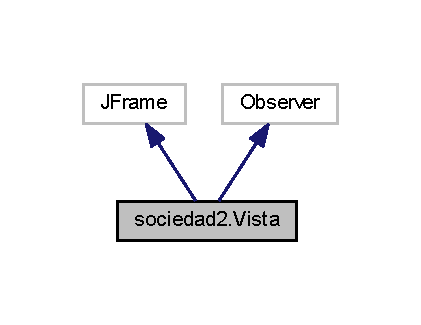
\includegraphics[width=202pt]{classsociedad2_1_1_vista__inherit__graph}
\end{center}
\end{figure}


Collaboration diagram for sociedad2.\+Vista\+:
\nopagebreak
\begin{figure}[H]
\begin{center}
\leavevmode
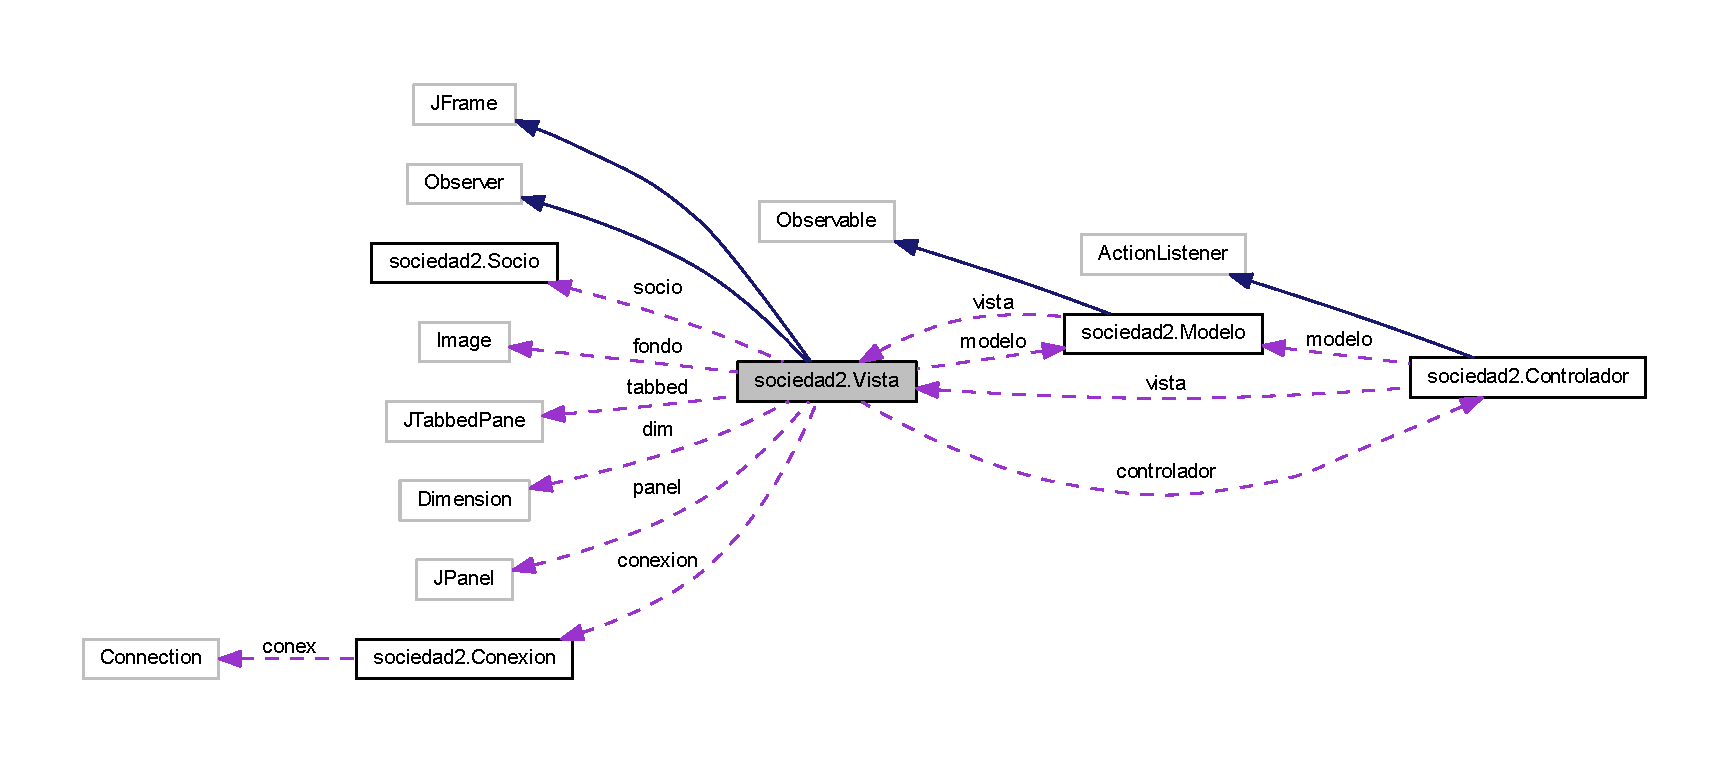
\includegraphics[width=350pt]{classsociedad2_1_1_vista__coll__graph}
\end{center}
\end{figure}
\subsection*{Public Member Functions}
\begin{DoxyCompactItemize}
\item 
\mbox{\hyperlink{classsociedad2_1_1_vista_aada4eb29ed80892f3c4687e867f77587}{Vista}} (String s)
\item 
\mbox{\hyperlink{classsociedad2_1_1_conexion}{Conexion}} \mbox{\hyperlink{classsociedad2_1_1_vista_a9d018d249c3888a62f7ba905cfb50d3a}{get\+Conexion}} ()
\item 
void \mbox{\hyperlink{classsociedad2_1_1_vista_a103a6cd3dba96b73a7ce663d8c91dce6}{go}} (\mbox{\hyperlink{classsociedad2_1_1_socio}{Socio}} socio)
\item 
\mbox{\hyperlink{classsociedad2_1_1_socio}{Socio}} \mbox{\hyperlink{classsociedad2_1_1_vista_abb81b93cc2a77eec1a011a6b66d2097e}{get\+Socio}} ()
\item 
void \mbox{\hyperlink{classsociedad2_1_1_vista_a48b32507f61975d72ef37f0ee69e5e5c}{update}} (Observable o, Object arg)
\end{DoxyCompactItemize}
\subsection*{Static Public Member Functions}
\begin{DoxyCompactItemize}
\item 
static void \mbox{\hyperlink{classsociedad2_1_1_vista_a9d4ba8e7d2fc1e8f48374eb484ddb76c}{main}} (String\mbox{[}$\,$\mbox{]} args)
\end{DoxyCompactItemize}


\subsection{Detailed Description}


Definition at line 32 of file Vista.\+java.



\subsection{Constructor \& Destructor Documentation}
\mbox{\Hypertarget{classsociedad2_1_1_vista_aada4eb29ed80892f3c4687e867f77587}\label{classsociedad2_1_1_vista_aada4eb29ed80892f3c4687e867f77587}} 
\index{sociedad2\+::\+Vista@{sociedad2\+::\+Vista}!Vista@{Vista}}
\index{Vista@{Vista}!sociedad2\+::\+Vista@{sociedad2\+::\+Vista}}
\subsubsection{\texorpdfstring{Vista()}{Vista()}}
{\footnotesize\ttfamily sociedad2.\+Vista.\+Vista (\begin{DoxyParamCaption}\item[{String}]{s }\end{DoxyParamCaption})}



Definition at line 43 of file Vista.\+java.



\subsection{Member Function Documentation}
\mbox{\Hypertarget{classsociedad2_1_1_vista_a9d018d249c3888a62f7ba905cfb50d3a}\label{classsociedad2_1_1_vista_a9d018d249c3888a62f7ba905cfb50d3a}} 
\index{sociedad2\+::\+Vista@{sociedad2\+::\+Vista}!get\+Conexion@{get\+Conexion}}
\index{get\+Conexion@{get\+Conexion}!sociedad2\+::\+Vista@{sociedad2\+::\+Vista}}
\subsubsection{\texorpdfstring{get\+Conexion()}{getConexion()}}
{\footnotesize\ttfamily \mbox{\hyperlink{classsociedad2_1_1_conexion}{Conexion}} sociedad2.\+Vista.\+get\+Conexion (\begin{DoxyParamCaption}{ }\end{DoxyParamCaption})}



Definition at line 74 of file Vista.\+java.

\mbox{\Hypertarget{classsociedad2_1_1_vista_abb81b93cc2a77eec1a011a6b66d2097e}\label{classsociedad2_1_1_vista_abb81b93cc2a77eec1a011a6b66d2097e}} 
\index{sociedad2\+::\+Vista@{sociedad2\+::\+Vista}!get\+Socio@{get\+Socio}}
\index{get\+Socio@{get\+Socio}!sociedad2\+::\+Vista@{sociedad2\+::\+Vista}}
\subsubsection{\texorpdfstring{get\+Socio()}{getSocio()}}
{\footnotesize\ttfamily \mbox{\hyperlink{classsociedad2_1_1_socio}{Socio}} sociedad2.\+Vista.\+get\+Socio (\begin{DoxyParamCaption}{ }\end{DoxyParamCaption})}



Definition at line 131 of file Vista.\+java.

\mbox{\Hypertarget{classsociedad2_1_1_vista_a103a6cd3dba96b73a7ce663d8c91dce6}\label{classsociedad2_1_1_vista_a103a6cd3dba96b73a7ce663d8c91dce6}} 
\index{sociedad2\+::\+Vista@{sociedad2\+::\+Vista}!go@{go}}
\index{go@{go}!sociedad2\+::\+Vista@{sociedad2\+::\+Vista}}
\subsubsection{\texorpdfstring{go()}{go()}}
{\footnotesize\ttfamily void sociedad2.\+Vista.\+go (\begin{DoxyParamCaption}\item[{\mbox{\hyperlink{classsociedad2_1_1_socio}{Socio}}}]{socio }\end{DoxyParamCaption})}



Definition at line 125 of file Vista.\+java.

\mbox{\Hypertarget{classsociedad2_1_1_vista_a9d4ba8e7d2fc1e8f48374eb484ddb76c}\label{classsociedad2_1_1_vista_a9d4ba8e7d2fc1e8f48374eb484ddb76c}} 
\index{sociedad2\+::\+Vista@{sociedad2\+::\+Vista}!main@{main}}
\index{main@{main}!sociedad2\+::\+Vista@{sociedad2\+::\+Vista}}
\subsubsection{\texorpdfstring{main()}{main()}}
{\footnotesize\ttfamily static void sociedad2.\+Vista.\+main (\begin{DoxyParamCaption}\item[{String \mbox{[}$\,$\mbox{]}}]{args }\end{DoxyParamCaption})\hspace{0.3cm}{\ttfamily [static]}}



Definition at line 137 of file Vista.\+java.

\mbox{\Hypertarget{classsociedad2_1_1_vista_a48b32507f61975d72ef37f0ee69e5e5c}\label{classsociedad2_1_1_vista_a48b32507f61975d72ef37f0ee69e5e5c}} 
\index{sociedad2\+::\+Vista@{sociedad2\+::\+Vista}!update@{update}}
\index{update@{update}!sociedad2\+::\+Vista@{sociedad2\+::\+Vista}}
\subsubsection{\texorpdfstring{update()}{update()}}
{\footnotesize\ttfamily void sociedad2.\+Vista.\+update (\begin{DoxyParamCaption}\item[{Observable}]{o,  }\item[{Object}]{arg }\end{DoxyParamCaption})}



Definition at line 161 of file Vista.\+java.



The documentation for this class was generated from the following file\+:\begin{DoxyCompactItemize}
\item 
E\+:/eclipse-\/workspace/\+Sociedad/src/sociedad2/\mbox{\hyperlink{_vista_8java}{Vista.\+java}}\end{DoxyCompactItemize}

\chapter{File Documentation}
\hypertarget{_categorias_8java}{}\section{E\+:/eclipse-\/workspace/\+Sociedad/src/sociedad2/\+Categorias.java File Reference}
\label{_categorias_8java}\index{E\+:/eclipse-\/workspace/\+Sociedad/src/sociedad2/\+Categorias.\+java@{E\+:/eclipse-\/workspace/\+Sociedad/src/sociedad2/\+Categorias.\+java}}
\subsection*{Classes}
\begin{DoxyCompactItemize}
\item 
class \mbox{\hyperlink{classsociedad2_1_1_categorias}{sociedad2.\+Categorias}}
\end{DoxyCompactItemize}
\subsection*{Packages}
\begin{DoxyCompactItemize}
\item 
package \mbox{\hyperlink{namespacesociedad2}{sociedad2}}
\begin{DoxyCompactList}\small\item\em Packages. \end{DoxyCompactList}\end{DoxyCompactItemize}

\hypertarget{_conexion_8java}{}\section{E\+:/eclipse-\/workspace/\+Sociedad/src/sociedad2/\+Conexion.java File Reference}
\label{_conexion_8java}\index{E\+:/eclipse-\/workspace/\+Sociedad/src/sociedad2/\+Conexion.\+java@{E\+:/eclipse-\/workspace/\+Sociedad/src/sociedad2/\+Conexion.\+java}}
\subsection*{Classes}
\begin{DoxyCompactItemize}
\item 
class \mbox{\hyperlink{classsociedad2_1_1_conexion}{sociedad2.\+Conexion}}
\end{DoxyCompactItemize}
\subsection*{Packages}
\begin{DoxyCompactItemize}
\item 
package \mbox{\hyperlink{namespacesociedad2}{sociedad2}}
\end{DoxyCompactItemize}

\hypertarget{_controlador_8java}{}\section{E\+:/eclipse-\/workspace/\+Sociedad/src/sociedad2/\+Controlador.java File Reference}
\label{_controlador_8java}\index{E\+:/eclipse-\/workspace/\+Sociedad/src/sociedad2/\+Controlador.\+java@{E\+:/eclipse-\/workspace/\+Sociedad/src/sociedad2/\+Controlador.\+java}}


Class in which we respond to user interactions.  


\subsection*{Classes}
\begin{DoxyCompactItemize}
\item 
class \mbox{\hyperlink{classsociedad2_1_1_controlador}{sociedad2.\+Controlador}}
\begin{DoxyCompactList}\small\item\em \mbox{\hyperlink{classsociedad2_1_1_controlador}{Controlador}} class. \end{DoxyCompactList}\end{DoxyCompactItemize}
\subsection*{Packages}
\begin{DoxyCompactItemize}
\item 
package \mbox{\hyperlink{namespacesociedad2}{sociedad2}}
\begin{DoxyCompactList}\small\item\em Packages. \end{DoxyCompactList}\end{DoxyCompactItemize}


\subsection{Detailed Description}
Class in which we respond to user interactions. 

\begin{DoxyAuthor}{Authors}
Name $\vert$ Surname $\vert$ Email $\vert$ -\/-\/-\/-\/-\/-\/-\/-\/-\/-\/--- $\vert$ -\/-\/-\/-\/-\/-\/-\/-\/-\/-\/-\/--- $\vert$ -\/-\/-\/-\/-\/-\/-\/-\/-\/-\/-\/-\/-\/-\/-\/-\/-\/-\/-\/-\/-\/-\/-\/-\/-\/-\/-\/-\/-\/-\/-\/-\/-\/--- $\vert$ Marcos Azcarate \href{mailto:marcos.azcarate@alumni.mondragon.edu}{\tt marcos.\+azcarate@alumni.\+mondragon.\+edu} 
\end{DoxyAuthor}
\begin{DoxyDate}{Date}
05/10/2018 
\end{DoxyDate}

\hypertarget{_dialogo_editar_producto_8java}{}\section{E\+:/eclipse-\/workspace/\+Sociedad/src/sociedad2/\+Dialogo\+Editar\+Producto.java File Reference}
\label{_dialogo_editar_producto_8java}\index{E\+:/eclipse-\/workspace/\+Sociedad/src/sociedad2/\+Dialogo\+Editar\+Producto.\+java@{E\+:/eclipse-\/workspace/\+Sociedad/src/sociedad2/\+Dialogo\+Editar\+Producto.\+java}}
\subsection*{Classes}
\begin{DoxyCompactItemize}
\item 
class \mbox{\hyperlink{classsociedad2_1_1_dialogo_editar_producto}{sociedad2.\+Dialogo\+Editar\+Producto}}
\end{DoxyCompactItemize}
\subsection*{Packages}
\begin{DoxyCompactItemize}
\item 
package \mbox{\hyperlink{namespacesociedad2}{sociedad2}}
\begin{DoxyCompactList}\small\item\em Packages. \end{DoxyCompactList}\end{DoxyCompactItemize}

\hypertarget{_dialogo_editar_socio_8java}{}\section{E\+:/eclipse-\/workspace/\+Sociedad/src/sociedad2/\+Dialogo\+Editar\+Socio.java File Reference}
\label{_dialogo_editar_socio_8java}\index{E\+:/eclipse-\/workspace/\+Sociedad/src/sociedad2/\+Dialogo\+Editar\+Socio.\+java@{E\+:/eclipse-\/workspace/\+Sociedad/src/sociedad2/\+Dialogo\+Editar\+Socio.\+java}}
\subsection*{Classes}
\begin{DoxyCompactItemize}
\item 
class \mbox{\hyperlink{classsociedad2_1_1_dialogo_editar_socio}{sociedad2.\+Dialogo\+Editar\+Socio}}
\end{DoxyCompactItemize}
\subsection*{Packages}
\begin{DoxyCompactItemize}
\item 
package \mbox{\hyperlink{namespacesociedad2}{sociedad2}}
\end{DoxyCompactItemize}

\hypertarget{_dialogo_insertar_producto_8java}{}\section{E\+:/eclipse-\/workspace/\+Sociedad/src/sociedad2/\+Dialogo\+Insertar\+Producto.java File Reference}
\label{_dialogo_insertar_producto_8java}\index{E\+:/eclipse-\/workspace/\+Sociedad/src/sociedad2/\+Dialogo\+Insertar\+Producto.\+java@{E\+:/eclipse-\/workspace/\+Sociedad/src/sociedad2/\+Dialogo\+Insertar\+Producto.\+java}}
\subsection*{Classes}
\begin{DoxyCompactItemize}
\item 
class \mbox{\hyperlink{classsociedad2_1_1_dialogo_insertar_producto}{sociedad2.\+Dialogo\+Insertar\+Producto}}
\end{DoxyCompactItemize}
\subsection*{Packages}
\begin{DoxyCompactItemize}
\item 
package \mbox{\hyperlink{namespacesociedad2}{sociedad2}}
\end{DoxyCompactItemize}

\hypertarget{_dialogo_insertar_socio_8java}{}\section{E\+:/eclipse-\/workspace/\+Sociedad/src/sociedad2/\+Dialogo\+Insertar\+Socio.java File Reference}
\label{_dialogo_insertar_socio_8java}\index{E\+:/eclipse-\/workspace/\+Sociedad/src/sociedad2/\+Dialogo\+Insertar\+Socio.\+java@{E\+:/eclipse-\/workspace/\+Sociedad/src/sociedad2/\+Dialogo\+Insertar\+Socio.\+java}}
\subsection*{Classes}
\begin{DoxyCompactItemize}
\item 
class \mbox{\hyperlink{classsociedad2_1_1_dialogo_insertar_socio}{sociedad2.\+Dialogo\+Insertar\+Socio}}
\end{DoxyCompactItemize}
\subsection*{Packages}
\begin{DoxyCompactItemize}
\item 
package \mbox{\hyperlink{namespacesociedad2}{sociedad2}}
\begin{DoxyCompactList}\small\item\em Packages. \end{DoxyCompactList}\end{DoxyCompactItemize}

\hypertarget{_dialogo_registrar_consumicion_8java}{}\section{E\+:/eclipse-\/workspace/\+Sociedad/src/sociedad2/\+Dialogo\+Registrar\+Consumicion.java File Reference}
\label{_dialogo_registrar_consumicion_8java}\index{E\+:/eclipse-\/workspace/\+Sociedad/src/sociedad2/\+Dialogo\+Registrar\+Consumicion.\+java@{E\+:/eclipse-\/workspace/\+Sociedad/src/sociedad2/\+Dialogo\+Registrar\+Consumicion.\+java}}
\subsection*{Classes}
\begin{DoxyCompactItemize}
\item 
class \mbox{\hyperlink{classsociedad2_1_1_dialogo_registrar_consumicion}{sociedad2.\+Dialogo\+Registrar\+Consumicion}}
\end{DoxyCompactItemize}
\subsection*{Packages}
\begin{DoxyCompactItemize}
\item 
package \mbox{\hyperlink{namespacesociedad2}{sociedad2}}
\end{DoxyCompactItemize}

\hypertarget{_dialogo_ver_producto_8java}{}\section{E\+:/eclipse-\/workspace/\+Sociedad/src/sociedad2/\+Dialogo\+Ver\+Producto.java File Reference}
\label{_dialogo_ver_producto_8java}\index{E\+:/eclipse-\/workspace/\+Sociedad/src/sociedad2/\+Dialogo\+Ver\+Producto.\+java@{E\+:/eclipse-\/workspace/\+Sociedad/src/sociedad2/\+Dialogo\+Ver\+Producto.\+java}}
\subsection*{Classes}
\begin{DoxyCompactItemize}
\item 
class \mbox{\hyperlink{classsociedad2_1_1_dialogo_ver_producto}{sociedad2.\+Dialogo\+Ver\+Producto}}
\end{DoxyCompactItemize}
\subsection*{Packages}
\begin{DoxyCompactItemize}
\item 
package \mbox{\hyperlink{namespacesociedad2}{sociedad2}}
\begin{DoxyCompactList}\small\item\em Packages. \end{DoxyCompactList}\end{DoxyCompactItemize}

\hypertarget{_dialogo_ver_productos_baja_8java}{}\section{E\+:/eclipse-\/workspace/\+Sociedad/src/sociedad2/\+Dialogo\+Ver\+Productos\+Baja.java File Reference}
\label{_dialogo_ver_productos_baja_8java}\index{E\+:/eclipse-\/workspace/\+Sociedad/src/sociedad2/\+Dialogo\+Ver\+Productos\+Baja.\+java@{E\+:/eclipse-\/workspace/\+Sociedad/src/sociedad2/\+Dialogo\+Ver\+Productos\+Baja.\+java}}
\subsection*{Classes}
\begin{DoxyCompactItemize}
\item 
class \mbox{\hyperlink{classsociedad2_1_1_dialogo_ver_productos_baja}{sociedad2.\+Dialogo\+Ver\+Productos\+Baja}}
\end{DoxyCompactItemize}
\subsection*{Packages}
\begin{DoxyCompactItemize}
\item 
package \mbox{\hyperlink{namespacesociedad2}{sociedad2}}
\end{DoxyCompactItemize}

\hypertarget{_dialogo_ver_socio_8java}{}\section{E\+:/eclipse-\/workspace/\+Sociedad/src/sociedad2/\+Dialogo\+Ver\+Socio.java File Reference}
\label{_dialogo_ver_socio_8java}\index{E\+:/eclipse-\/workspace/\+Sociedad/src/sociedad2/\+Dialogo\+Ver\+Socio.\+java@{E\+:/eclipse-\/workspace/\+Sociedad/src/sociedad2/\+Dialogo\+Ver\+Socio.\+java}}
\subsection*{Classes}
\begin{DoxyCompactItemize}
\item 
class \mbox{\hyperlink{classsociedad2_1_1_dialogo_ver_socio}{sociedad2.\+Dialogo\+Ver\+Socio}}
\end{DoxyCompactItemize}
\subsection*{Packages}
\begin{DoxyCompactItemize}
\item 
package \mbox{\hyperlink{namespacesociedad2}{sociedad2}}
\begin{DoxyCompactList}\small\item\em Packages. \end{DoxyCompactList}\end{DoxyCompactItemize}

\hypertarget{_dialogo_ver_socios_baja_8java}{}\section{E\+:/eclipse-\/workspace/\+Sociedad/src/sociedad2/\+Dialogo\+Ver\+Socios\+Baja.java File Reference}
\label{_dialogo_ver_socios_baja_8java}\index{E\+:/eclipse-\/workspace/\+Sociedad/src/sociedad2/\+Dialogo\+Ver\+Socios\+Baja.\+java@{E\+:/eclipse-\/workspace/\+Sociedad/src/sociedad2/\+Dialogo\+Ver\+Socios\+Baja.\+java}}
\subsection*{Classes}
\begin{DoxyCompactItemize}
\item 
class \mbox{\hyperlink{classsociedad2_1_1_dialogo_ver_socios_baja}{sociedad2.\+Dialogo\+Ver\+Socios\+Baja}}
\end{DoxyCompactItemize}
\subsection*{Packages}
\begin{DoxyCompactItemize}
\item 
package \mbox{\hyperlink{namespacesociedad2}{sociedad2}}
\end{DoxyCompactItemize}

\hypertarget{_login_8java}{}\section{E\+:/eclipse-\/workspace/\+Sociedad/src/sociedad2/\+Login.java File Reference}
\label{_login_8java}\index{E\+:/eclipse-\/workspace/\+Sociedad/src/sociedad2/\+Login.\+java@{E\+:/eclipse-\/workspace/\+Sociedad/src/sociedad2/\+Login.\+java}}
\subsection*{Classes}
\begin{DoxyCompactItemize}
\item 
class \mbox{\hyperlink{classsociedad2_1_1_login}{sociedad2.\+Login}}
\end{DoxyCompactItemize}
\subsection*{Packages}
\begin{DoxyCompactItemize}
\item 
package \mbox{\hyperlink{namespacesociedad2}{sociedad2}}
\end{DoxyCompactItemize}

\hypertarget{_mi_adaptador_8java}{}\section{E\+:/eclipse-\/workspace/\+Sociedad/src/sociedad2/\+Mi\+Adaptador.java File Reference}
\label{_mi_adaptador_8java}\index{E\+:/eclipse-\/workspace/\+Sociedad/src/sociedad2/\+Mi\+Adaptador.\+java@{E\+:/eclipse-\/workspace/\+Sociedad/src/sociedad2/\+Mi\+Adaptador.\+java}}
\subsection*{Classes}
\begin{DoxyCompactItemize}
\item 
class \mbox{\hyperlink{classsociedad2_1_1_mi_adaptador}{sociedad2.\+Mi\+Adaptador}}
\end{DoxyCompactItemize}
\subsection*{Packages}
\begin{DoxyCompactItemize}
\item 
package \mbox{\hyperlink{namespacesociedad2}{sociedad2}}
\end{DoxyCompactItemize}

\hypertarget{_mi_adaptador_producto_8java}{}\section{E\+:/eclipse-\/workspace/\+Sociedad/src/sociedad2/\+Mi\+Adaptador\+Producto.java File Reference}
\label{_mi_adaptador_producto_8java}\index{E\+:/eclipse-\/workspace/\+Sociedad/src/sociedad2/\+Mi\+Adaptador\+Producto.\+java@{E\+:/eclipse-\/workspace/\+Sociedad/src/sociedad2/\+Mi\+Adaptador\+Producto.\+java}}
\subsection*{Classes}
\begin{DoxyCompactItemize}
\item 
class \mbox{\hyperlink{classsociedad2_1_1_mi_adaptador_producto}{sociedad2.\+Mi\+Adaptador\+Producto}}
\end{DoxyCompactItemize}
\subsection*{Packages}
\begin{DoxyCompactItemize}
\item 
package \mbox{\hyperlink{namespacesociedad2}{sociedad2}}
\end{DoxyCompactItemize}

\hypertarget{_mi_adaptador_registrar_consumicion_8java}{}\section{E\+:/eclipse-\/workspace/\+Sociedad/src/sociedad2/\+Mi\+Adaptador\+Registrar\+Consumicion.java File Reference}
\label{_mi_adaptador_registrar_consumicion_8java}\index{E\+:/eclipse-\/workspace/\+Sociedad/src/sociedad2/\+Mi\+Adaptador\+Registrar\+Consumicion.\+java@{E\+:/eclipse-\/workspace/\+Sociedad/src/sociedad2/\+Mi\+Adaptador\+Registrar\+Consumicion.\+java}}
\subsection*{Classes}
\begin{DoxyCompactItemize}
\item 
class \mbox{\hyperlink{classsociedad2_1_1_mi_adaptador_registrar_consumicion}{sociedad2.\+Mi\+Adaptador\+Registrar\+Consumicion}}
\end{DoxyCompactItemize}
\subsection*{Packages}
\begin{DoxyCompactItemize}
\item 
package \mbox{\hyperlink{namespacesociedad2}{sociedad2}}
\begin{DoxyCompactList}\small\item\em Packages. \end{DoxyCompactList}\end{DoxyCompactItemize}

\hypertarget{_mi_panel_8java}{}\section{E\+:/eclipse-\/workspace/\+Sociedad/src/sociedad2/\+Mi\+Panel.java File Reference}
\label{_mi_panel_8java}\index{E\+:/eclipse-\/workspace/\+Sociedad/src/sociedad2/\+Mi\+Panel.\+java@{E\+:/eclipse-\/workspace/\+Sociedad/src/sociedad2/\+Mi\+Panel.\+java}}
\subsection*{Classes}
\begin{DoxyCompactItemize}
\item 
class \mbox{\hyperlink{classsociedad2_1_1_mi_panel}{sociedad2.\+Mi\+Panel}}
\end{DoxyCompactItemize}
\subsection*{Packages}
\begin{DoxyCompactItemize}
\item 
package \mbox{\hyperlink{namespacesociedad2}{sociedad2}}
\end{DoxyCompactItemize}

\hypertarget{_modelo_8java}{}\section{E\+:/eclipse-\/workspace/\+Sociedad/src/sociedad2/\+Modelo.java File Reference}
\label{_modelo_8java}\index{E\+:/eclipse-\/workspace/\+Sociedad/src/sociedad2/\+Modelo.\+java@{E\+:/eclipse-\/workspace/\+Sociedad/src/sociedad2/\+Modelo.\+java}}
\subsection*{Classes}
\begin{DoxyCompactItemize}
\item 
class \mbox{\hyperlink{classsociedad2_1_1_modelo}{sociedad2.\+Modelo}}
\end{DoxyCompactItemize}
\subsection*{Packages}
\begin{DoxyCompactItemize}
\item 
package \mbox{\hyperlink{namespacesociedad2}{sociedad2}}
\end{DoxyCompactItemize}

\hypertarget{_producto_8java}{}\section{E\+:/eclipse-\/workspace/\+Sociedad/src/sociedad2/\+Producto.java File Reference}
\label{_producto_8java}\index{E\+:/eclipse-\/workspace/\+Sociedad/src/sociedad2/\+Producto.\+java@{E\+:/eclipse-\/workspace/\+Sociedad/src/sociedad2/\+Producto.\+java}}
\subsection*{Classes}
\begin{DoxyCompactItemize}
\item 
class \mbox{\hyperlink{classsociedad2_1_1_producto}{sociedad2.\+Producto}}
\end{DoxyCompactItemize}
\subsection*{Packages}
\begin{DoxyCompactItemize}
\item 
package \mbox{\hyperlink{namespacesociedad2}{sociedad2}}
\begin{DoxyCompactList}\small\item\em Packages. \end{DoxyCompactList}\end{DoxyCompactItemize}

\hypertarget{_producto_consumicion_8java}{}\section{E\+:/eclipse-\/workspace/\+Sociedad/src/sociedad2/\+Producto\+Consumicion.java File Reference}
\label{_producto_consumicion_8java}\index{E\+:/eclipse-\/workspace/\+Sociedad/src/sociedad2/\+Producto\+Consumicion.\+java@{E\+:/eclipse-\/workspace/\+Sociedad/src/sociedad2/\+Producto\+Consumicion.\+java}}
\subsection*{Classes}
\begin{DoxyCompactItemize}
\item 
class \mbox{\hyperlink{classsociedad2_1_1_producto_consumicion}{sociedad2.\+Producto\+Consumicion}}
\end{DoxyCompactItemize}
\subsection*{Packages}
\begin{DoxyCompactItemize}
\item 
package \mbox{\hyperlink{namespacesociedad2}{sociedad2}}
\end{DoxyCompactItemize}

\hypertarget{_socio_8java}{}\section{E\+:/eclipse-\/workspace/\+Sociedad/src/sociedad2/\+Socio.java File Reference}
\label{_socio_8java}\index{E\+:/eclipse-\/workspace/\+Sociedad/src/sociedad2/\+Socio.\+java@{E\+:/eclipse-\/workspace/\+Sociedad/src/sociedad2/\+Socio.\+java}}
\subsection*{Classes}
\begin{DoxyCompactItemize}
\item 
class \mbox{\hyperlink{classsociedad2_1_1_socio}{sociedad2.\+Socio}}
\end{DoxyCompactItemize}
\subsection*{Packages}
\begin{DoxyCompactItemize}
\item 
package \mbox{\hyperlink{namespacesociedad2}{sociedad2}}
\begin{DoxyCompactList}\small\item\em Packages. \end{DoxyCompactList}\end{DoxyCompactItemize}

\hypertarget{_vista_8java}{}\section{E\+:/eclipse-\/workspace/\+Sociedad/src/sociedad2/\+Vista.java File Reference}
\label{_vista_8java}\index{E\+:/eclipse-\/workspace/\+Sociedad/src/sociedad2/\+Vista.\+java@{E\+:/eclipse-\/workspace/\+Sociedad/src/sociedad2/\+Vista.\+java}}
\subsection*{Classes}
\begin{DoxyCompactItemize}
\item 
class \mbox{\hyperlink{classsociedad2_1_1_vista}{sociedad2.\+Vista}}
\end{DoxyCompactItemize}
\subsection*{Packages}
\begin{DoxyCompactItemize}
\item 
package \mbox{\hyperlink{namespacesociedad2}{sociedad2}}
\begin{DoxyCompactList}\small\item\em Packages. \end{DoxyCompactList}\end{DoxyCompactItemize}

%--- End generated contents ---

% Index
\backmatter
\newpage
\phantomsection
\clearemptydoublepage
\addcontentsline{toc}{chapter}{Index}
\printindex

\end{document}
